\chapter{Une approche cartographique des textiles pour saisir leur répartition et leurs mobilités}
\markboth{}{}

\epigraph{\textquotedblleft Textiles move easily and designs and structures provoke imitations. Taking into consideration the style of the designs and the conditions of their creation will open new potential lines of fruitful research.\textquotedblright}{Sophie Desrosiers, 2014, \og Highland Complementary-Warp Weaving and the Lima Style in the Central Coast of Peru, ca. 200-650 C.E. \fg, p.~11.}


\section[Pré-traitement des données pour l'analyse géographique]{Pré-traitement des données pour l'analyse géographique}

\subsection{Homogénéiser les données}

À la suite de la récupération des données, une vue d'ensemble sur celles-ci nous permettra de mieux saisir leur organisation et leur constitution, ainsi que les pré-traitements nécessaires au travail d'analyse.

\subsubsection{Traitement des données manquantes}

La première étape de traitement des données consiste à inspecter la quantité de données manquantes pour chaque catégorie. 
Dans le cas de notre base de données, les données manquantes n'étaient pas toutes renseignées de la même manière. 
Certaines catégories étaient vides mais pour d'autres l'absence de données était indiquée par des chaînes de caractères (ensemble de lettres) et donc considérée comme une information au moment du traitement des données. 
J'ai détecté trois indications de ce type à partir de la reconstitution de l'ontologie de la base de données : \og \textit{unknown}\fg, \og \textit{unindentified fragment}\fg \:et \og \textit{NO DESCRIPTION AVAILABLE}\fg. Comme nous pouvons le voir, ces trois expressions n'indiquent pas l'absence de la même manière. La première indique une absence de connaissances (probablement lié au manque de contexte de certains textiles), la seconde indique l'impossibilité d'identifier l'utilité des textiles fragmentaires et la dernière correspond plutôt à une absence de données au sein de la base. Même si elles sont porteuses de sens, ces expressions sont remplacées par une valeur nulle (NaN) pour notre analyse, qui sera prise en compte comme telle au moment du traitement de données. Cette modification permet d'avoir une vision d'ensemble sur la base de données, de connaître le nombre d'informations disponibles pour chaque catégorie et donc de détecter celles qui sont les plus représentatives pour mener une analyse.

Cette modification permet d'obtenir le pourcentage réel de données manquantes de chaque catégorie comme nous pouvons le voir dans le tableau suivant : \\

\begin{table}[!h]
    \begin{tabular}{|p{0.3\textwidth}|p{0.3\textwidth}|p{0.3\textwidth}|}
        \hline
        \textbf{Nom de la catégorie} & \textbf{Pourcentage initial de données manquantes} & \textbf{Pourcentage final de données manquantes } \\ [3ex]\hline
         \textit{Style} & 22,55\% & 25,86\%\\[1ex] \hline
           \textit{Culture}& 25,43\% & 28,45\% \\ [1ex]\hline
           \textit{Product}& 0\% & 4,45\% \\ [1ex]\hline
    \end{tabular}
    \caption{Données manquantes avant et après modification.}
    \label{tab:NaN}
\end{table}  

Après ce traitement, nous pouvons observer la répartition des données disponibles par catégories dans la base de données. En moyenne, les catégories ont 47,73\% de valeurs manquantes. Toutefois, nous pouvons observer que seules 9 catégories sont complètement vides, et que 5 catégories sont au-dessus de 80\% de valeur nulle. À l'inverse, 6 catégories sont complètes et 14 catégories sont en-dessous de 10\% de valeur nulle, la médiane se situant à 36,93\%. Connaître les données manquantes nous permet de déterminer les catégories avec lesquelles il sera possible de travailler de manière représentative.

\begin{figure}[!h]
	\begin{center}
		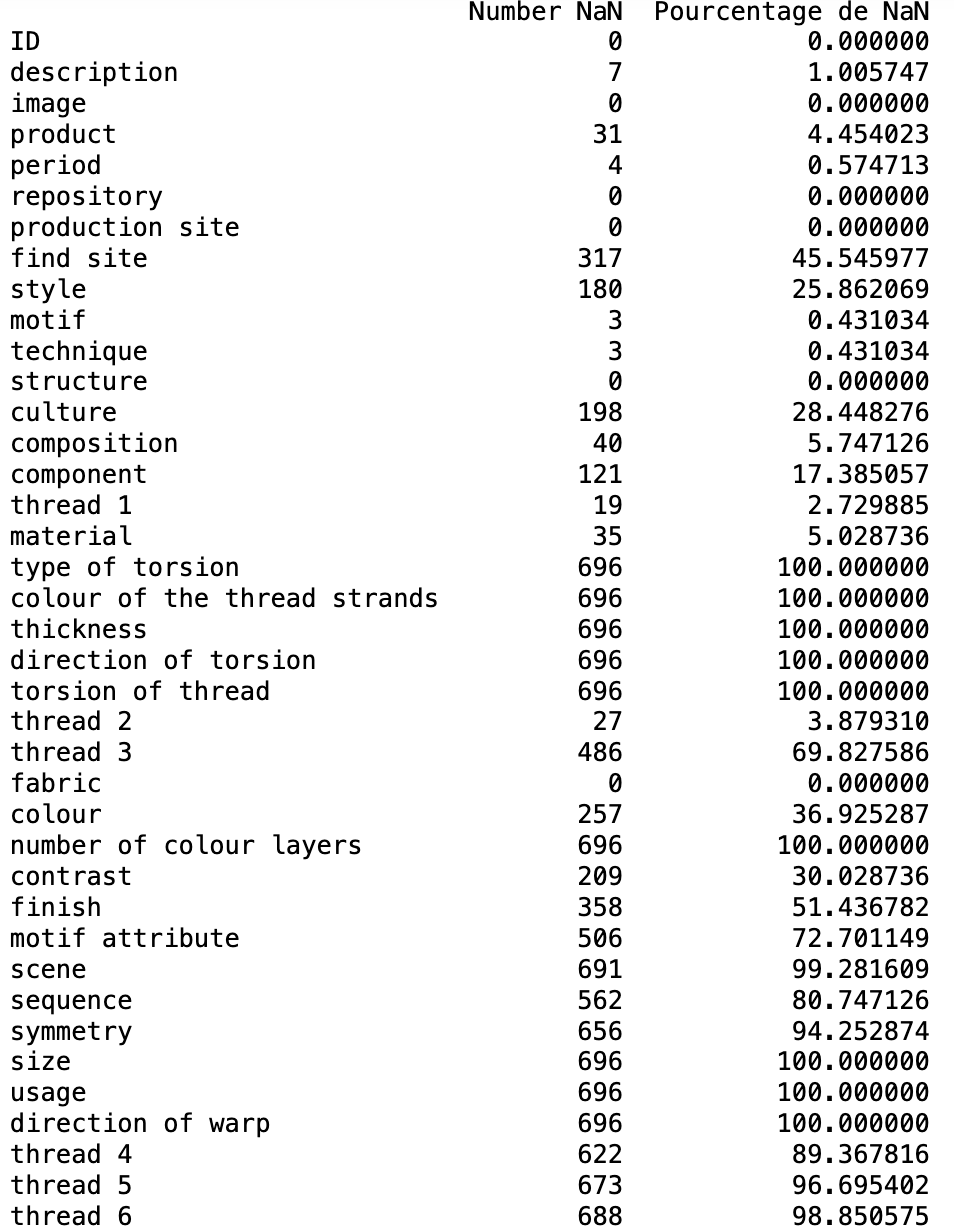
\includegraphics[width=9cm]{../images/NaN.png}
           	 \caption{Pourcentage de données manquantes par catégorie.}
           	 \label{NaN}
	 \end{center}
  \end{figure}


\clearpage


\subsubsection{Données historiques}

Un des intérêts du corpus étudié est sa profondeur historique qui permet une étude diachronique des pièces textiles. Les métadonnées associées aux pièces textiles nous fournissent la période de production de la pièce, ainsi qu'une datation approximative de cette même période pour 692 pièces (sur les 696 du corpus)\footnote{Voir le tableau récapitulatif des données indisponibles après traitement du tableur originel, image \ref{NaN}.}. Ces périodes reprennent la nomenclature archéologique traditionnellement utilisée pour les Andes, couvrant une temporalité allant de 1800 avant notre ère au temps présent.

\begin{figure}[!h]
	\begin{center}
		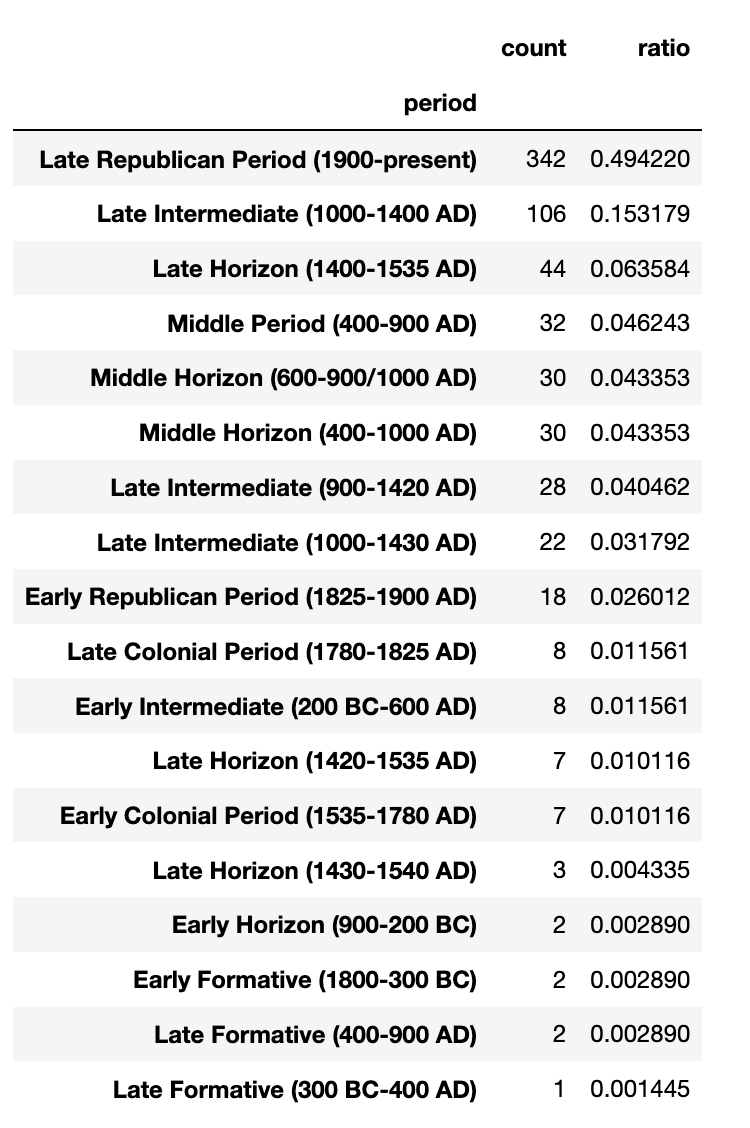
\includegraphics[width=10cm]{../images/periods_orig.png}
           	 \caption{Données chronologiques initiales}
           	 \label{chronoInit}
	 \end{center}
  \end{figure}
  
Malgré le recours à une ontologie lors de la création de la base de données, cette chronologie n'est pas uniformisée. Certaines périodes se superposent, d'autres couvrent la même période chronologique mais ne portent pas le même nom et certaines portent le même nom mais n'ont pas les mêmes dates de début et de fin, comme nous pouvons le voir sur le tableau \ref{chronoInit} et la frise chronologique \ref{chronoInitFri}. La variation des données biaise la compréhension statistique du corpus, c'est pourquoi il est nécessaire d'homogénéiser cette chronologie.
\clearpage

  \begin{figure}[!h]
	\begin{center}
		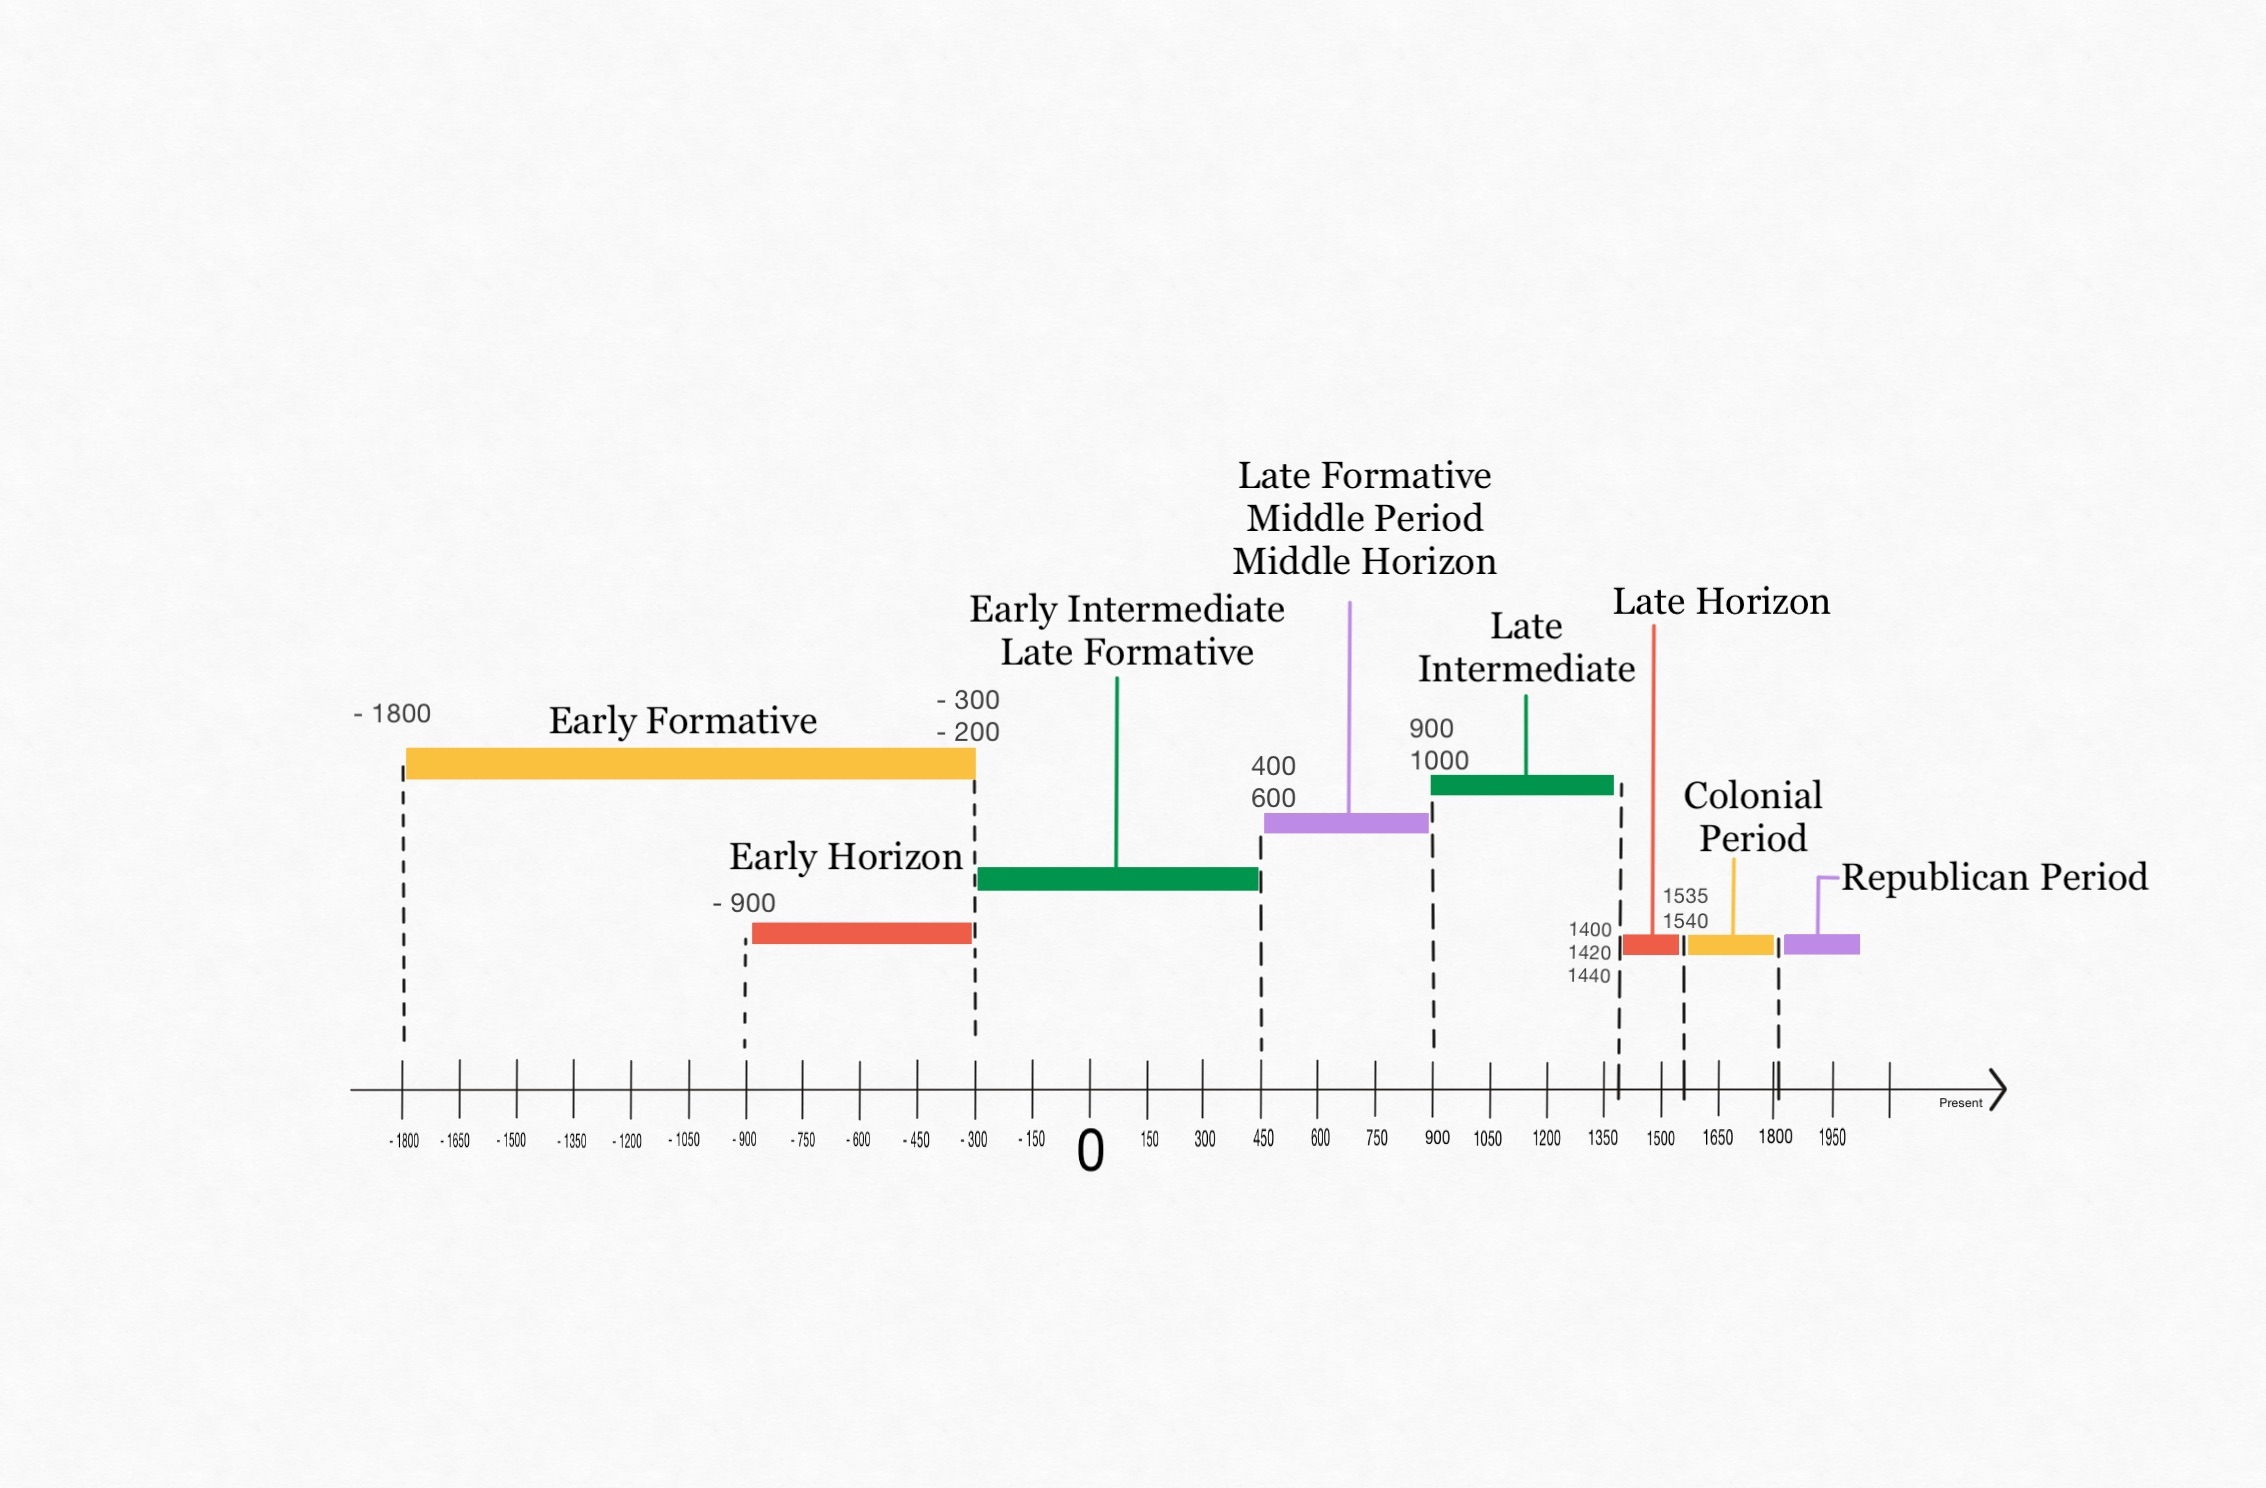
\includegraphics[width=15cm]{../images/FriseChronologiqueOrig.jpg}
           	 \caption{Frise chronologique représentant les données disponibles dans la base de données.}
           	 \label{chronoInitFri}
	 \end{center}
  \end{figure}


Ces difficultés de terminologie et de datation sont induites par le long débat académique qui a pris place entre différentes écoles d'archéologie andine. D'après l'historien et archéologue Gabriel Ramón Joffré, la périodisation en archéologie andine est nécessaire pour classifier les découvertes, mais elle est limitée par le manque de discussion dans la discipline autour des critères d'organisation chronologique\footnote{\cite[p.~7]{ramonjoffrePeriodificacionArqueologiaPeruana2005}}. Cela se traduit par une permanence des catégories définies au début de la discipline auxquelles s'ajoute une multitude de périodes hybrides accolant différents critères. Plus largement, la discipline se divise en deux courants de périodisation, d'une part les partisans de la périodisation évolutive et, d'autre part, ceux de la périodisation chronologique\footnote{Ibid., p.~8}. Ces deux courants ne s'opposent pas mais ont des fondements théoriques différents. En effet, la périodisation évolutive repose sur des critères économiques ou politiques, indiquant les évolutions des sociétés étudiées, alors que celle chronologique prend pour unique critère la temporalité relative des découvertes archéologiques. La compréhension des différents courants de périodisation nous permet de comprendre les choix chronologiques apparents dans la base de données et facilite l'homogénéisation des données. 

Les archéologues qui proposent les premières chronologies, à partir de la fin du \siecle{XIX} prennent pour références les zones géographiques où ils travaillent. Ainsi, Max Uhle et Alfred L. Kroeber proposent différentes chronologies à partir de leurs travaux sur la côte péruvienne (Pachacamac, vallées Moche...)\footnote{Ibid., p.~10}. Julio C. Tello, quant à lui, propose une chronologie à partir de la \textit{sierra}, les terres en altitude.
La deuxième génération d'archéologues péruviens et la troisième génération d'archéologues étrangers adoptent progressivement l'approche évolutionniste. Peu à peu \og la côte nord, et plus spécifiquement la séquence de la vallée de Virú, se convertit en modèle pour interpréter l'histoire de toute la zone andine\footnote{Ibid., p.~12]. Citation originale : \textquotedblleft \textit{la costa norte, y específicamente la secuencia del valle del Virú, se convirtió en el modelo para interpretar la historia de toda el área andina.}\textquotedblright}. \fg \:Toutefois, toujours selon Gabriel Ramón Joffré, l'approche évolutionniste pose problème puisqu'elle implique \og d'assumer la synchronie d'événements singuliers sur une large zone avec une -- supposée -- homogénéité séquentielle \footnote{\cite[p.~13]{ramonjoffrePeriodificacionArqueologiaPeruana2005}. Citation originale : \textquotedblleft \textit{se debe asumir sincronía de eventos semejantes en un área amplia con -- supuesta -- homogeneidad secuencial.}\textquotedblright}. \fg \: 

Dans les années 1960, l'archéologue étatsunien John Howland Rowe, qui avait souligné la difficulté d'obtenir une datation absolue des découvertes archéologiques\footnote{\cite{roweAbsoluteChronologyAndean1945}}, propose une périodisation relative, composée de 6 périodes\footnote{\cite[p.~627]{roweCulturalUnityDiversification1960}}. Il développe ces périodes à partir d'une chronologie relative entre la zone de référence et les zones étudiées, à partir de leurs similarités culturelles. Les pièces découvertes dans le même style sont considérées comme quasi-contemporaines. Les périodes sont donc des périodes larges car elles prennent en compte une temporalité de diffusion des styles : 

\begin{wraptable}{r}{0.6\textwidth}
    \centering
    \begin{tabular}{|c|c|}
        \hline
        \textbf{Classification J.H Rowe} & \textbf{Traductions françaises} \\[1ex] \hline
         \textit{Initial Period} & Période Initiale \\[1ex] \hline
          \textit{Early Horizon} & Horizon Ancien \\ [1ex]\hline
          \textit{Early Intermediate Period} & Période Intermédiaire Ancienne \\ [1ex]\hline
          \textit{Middle Horizon} &  Horizon Moyen \\[1ex] \hline
          \textit{Late Intermediate Period} &  Période Intermédiaire Récente\\[1ex] \hline
          \textit{Late Horizon} &  Horizon Récent \\[1ex] \hline
    \end{tabular}
    \caption{Tableau de la périodisation de J. H. Rowe (1960) et traductions françaises.}
    \label{tab:periodsTrad}
\end{wraptable} 
 
\begin{citer}
	Les périodes fondamentales du système péruvien sont assez longues, à l'exception de l'Horizon récent qui a duré environ 58 ans. Les périodes antérieures durent entre 300 et 700 ans\footnote{\cite[p.~50]{roweStagesPeriodsArchaeological1962}. Citation originale : \textquotedblleft \textit{The basic periods of the Peruvian system are quite long, except for the Late Horizon which lasted only 	about 58 years. The earlier periods range from 300 to 700 years in length. }\textquotedblright}.
\end{citer}

\noindent Le schéma chronologique de Rowe devient le cadre de référence de nombreuses prospections archéologiques dans les Andes\footnote{\cite[p.~19]{ramonjoffrePeriodificacionArqueologiaPeruana2005}}. Toutefois, une chronologie évolutionniste émerge comme modèle parallèle, proposée notamment par Luis Lumbreras, archéologue péruvien. Ce dernier est spécialiste des zones d'altitude qu'il prend comme références pour étendre sa chronologie aux découvertes archéologiques de la côte.

\begin{table}[!h]
   \centering
    \begin{tabular}{|p{0.3\textwidth}|p{0.3\textwidth}|p{0.3\textwidth}|}
         \cline{1-3}
         \multicolumn{2}{|c|}{ \textbf{Classification L. Lumbreras (et traduction)}} & \textbf{Classification J. H. Rowe} \\ [1ex]  \cline{1-3}
         \textit{Lítico} &  Litique & Pré-céramique \\ [1ex]\hline
          \textit{Arcaico (temprano, medio, tardío)} & Archaïque (ancien, moyen, tardif) & Pré-céramique \\ \hline
          \textit{Formativo (inferior, medio, superior)} & Formatif (inférieur, moyen, supérieur) & Période Initiale / Horizon Ancien \\ \hline
          \textit{Desarollos Regionales} & Développements régionaux &  Période Intermédiaire Ancienne\\[1ex] \hline
          \textit{Expansión Wari} & Expansion Wari &  Horizon Moyen \\[1ex] \hline
          \textit{Estados Regionales} & Stades régionaux & Période Intermédiaire Récente \\ [1ex]\hline
          \textit{Imperio del Tawantinsuyo} & Empire du \textit{Tawantinsuyu} & Horizon Récent \\ [1ex]\hline
    \end{tabular} 
    \caption{\centering Tableau de la périodisation de L. Lumbreras (1965), traductions françaises et équivalents simplifiés chez Rowe (1960).}
    \label{tab:periods}
\end{table}  

\clearpage

À la suite de ces propositions classificatoires, les différents archéologues continuent de mélanger les deux modèles, évolutionniste et chronologique. Par exemple, le terme de Formatif est parfois utilisé pour décrire la période Initiale, l'Horizon Ancien et la période Intermédiaire Ancienne (de 1500 avant notre ère à 200 après notre ère), libéré de toutes connotations évolutives\footnote{\cite[p.~22]{ramonjoffrePeriodificacionArqueologiaPeruana2005}}. 

Après le développement de la datation carbone qui permet une précision temporelle, bien que relative, des bornes chronologiques sont associées à chaque période de Rowe. Les variations de bornes chronologiques dans la base de données sont liées au point de référence de la chronologie. Ainsi, la période \og \textit{Late Formative}\fg, de 400 à 900 avant notre ère, correspond à la datation de cette période dans les vallées occidentales du sud du Pérou, alors que la datation de 300 avant notre ère à 400 après notre ère correspond à la datation de l'Altiplano bolivien\footnote{Romuald Housse, communication personnelle.}. Il en est de même pour le début de l'Horizon Récent qui correspond à la période d'extension de l'empire Inca : 1430 correspond au début de l'extension de la civilisation Inca autour de son foyer d'origine, Cuzco, alors que la date de 1470 correspond à la date de la chute de Chan Chan, capitale de l'empire côtier Chimú. 

\begin{table}[!h]
    \centering
    \begin{tabular}{|c|c|}
         \hline
        \textbf{Classification J.H Rowe} & \textbf{Consensus actuel de datation} \\[1ex] \hline         
        Période Initiale & 1800 - 900 avant notre ère  \\[1ex] \hline
         Horizon Ancien & 900 - 200 avant notre ère\\ [1ex]\hline
         Période Intermédiaire Ancienne & 200 avant notre ère - 600 \\[1ex] \hline
         Horizon Moyen & 600 - 1000 \\[1ex] \hline
          Période Intermédiaire Récente & 1000 - 1470 \\[1ex] \hline
         Horizon Récent & 1470 - 1535\\[1ex] \hline
    \end{tabular}
    \caption{\centering Tableau de la périodisation de J. H. Rowe (1960) et datation contemporaine à partir de A. Boissière, B, Faugère et N. Goepfert (éds., 2022).}
    \label{tab:periodsRowe}
\end{table}  

\begin{figure}[!h]
	\begin{center}
		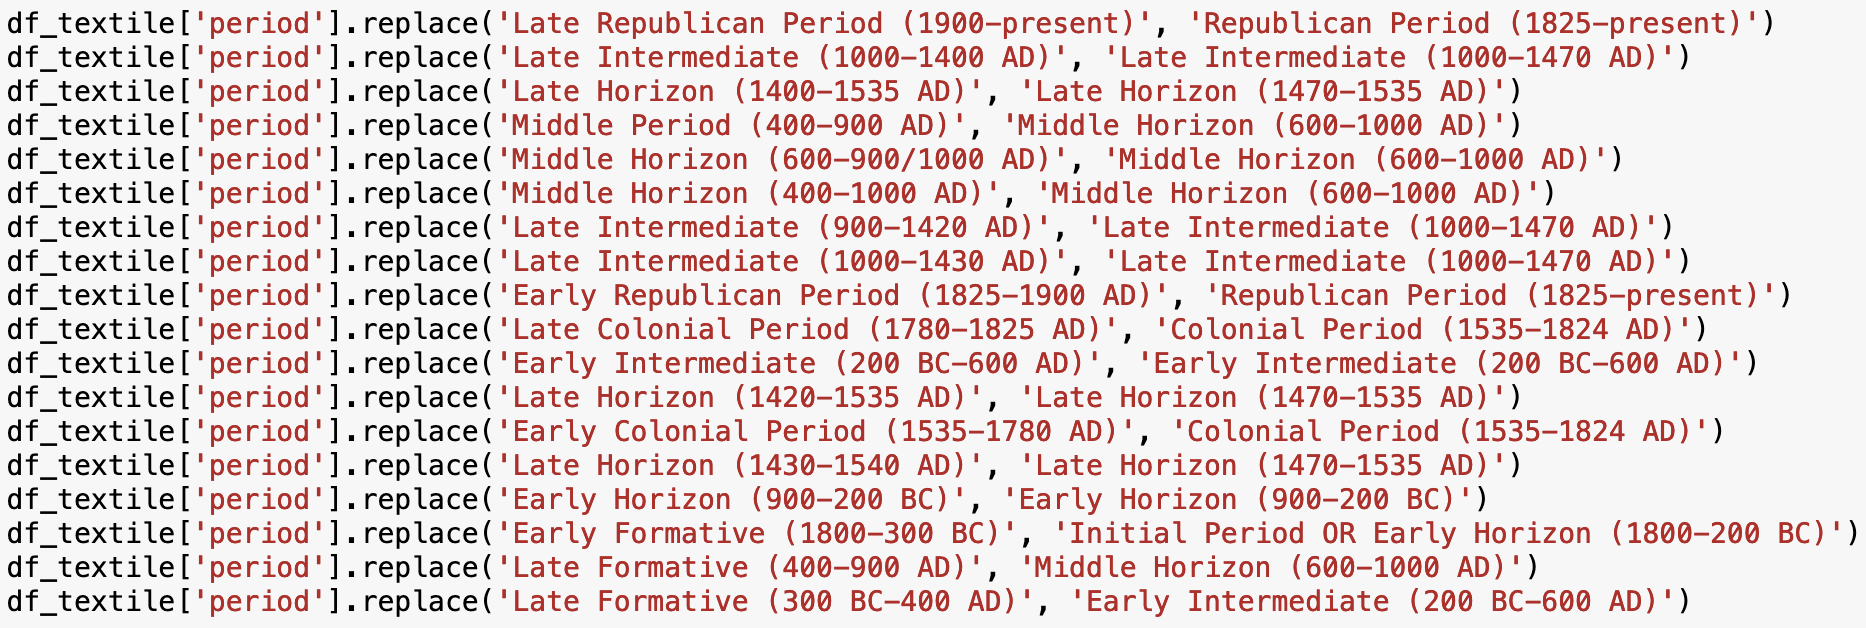
\includegraphics[width=15cm]{../images/periods_modif.png}
           	 \caption{Code utilisé pour modifier les données}
           	 \label{codeChrono}
	 \end{center}
  \end{figure}

La prise en compte de l'historiographie de la chronologie andine permet d'homogénéiser la chronologie de la base de données pour faciliter le traitement des données, sans pour autant perdre les informations chronologiques.
Nous passons alors de 18 périodes à 8 périodes. Cette réduction du nombre de plages chronologiques permet aussi une meilleure vue d'ensemble sur la répartition des données.

\clearpage

\begin{figure}[!h]
	\begin{center}
		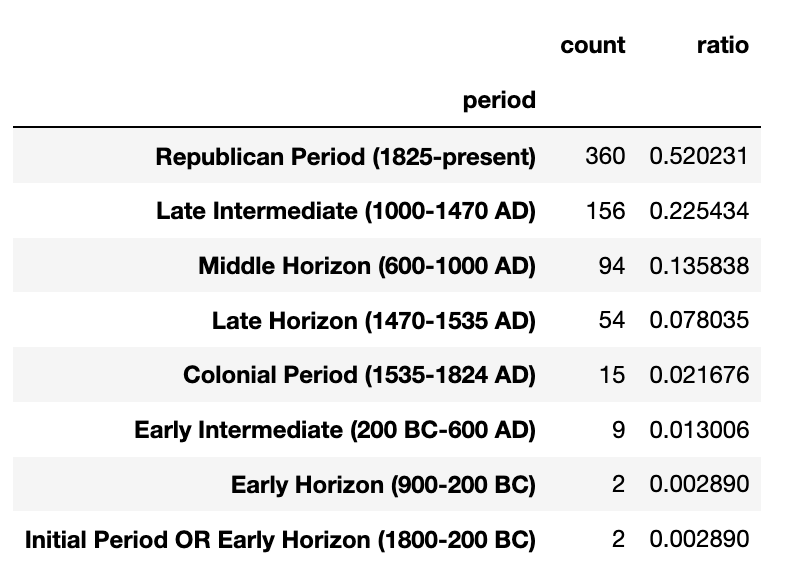
\includegraphics[width=10cm]{../images/periods_fin.png}
           	 \caption{Données chronologiques modifiées}
           	 \label{chronoFin}
	 \end{center}
  \end{figure}


  \begin{figure}[!h]
	\begin{center}
		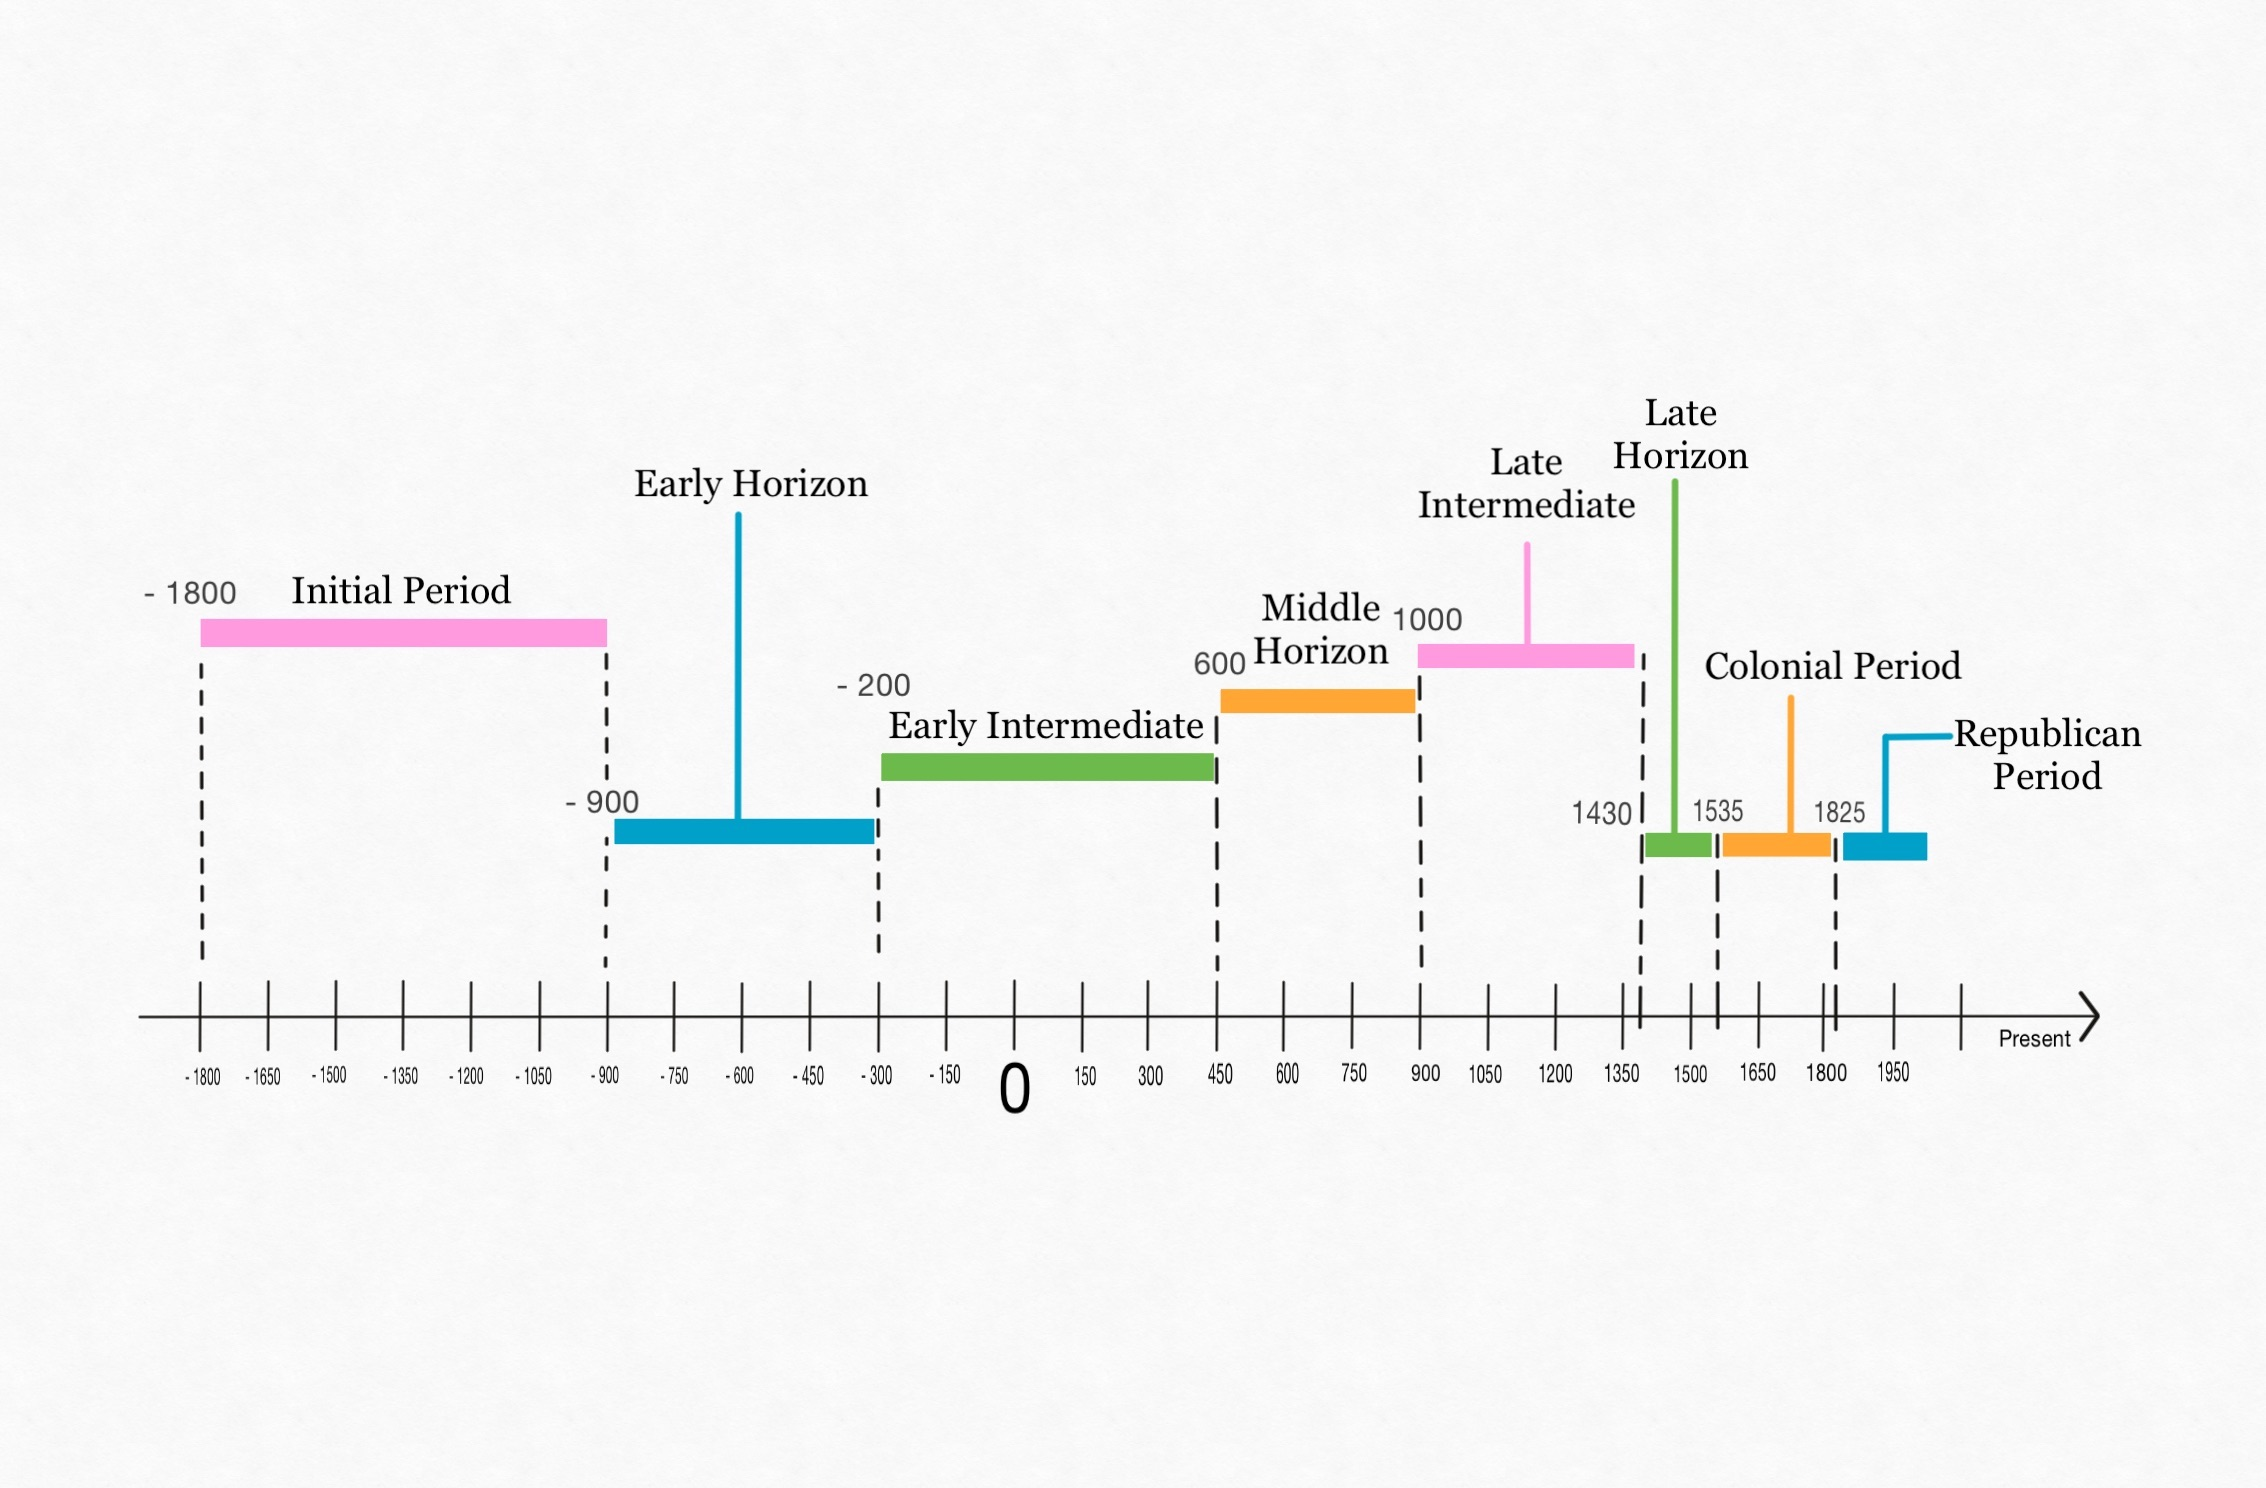
\includegraphics[width=15cm]{../images/FriseChronologique2.jpg}
           	 \caption{Frise chronologique représentant les données temporelles de la base de données après modification}
           	 \label{frisechronofinale}
	 \end{center}
  \end{figure}
  
Cette périodisation nous permettra ensuite d'avoir une approche diachronique des données. Cependant, nous ne devons pas perdre de vue que les périodes historiques restent des concepts vastes construits par les archéologues qui n'ont pas le même sens selon la zone des Andes étudiée. C'est pourquoi cette chronologie se doit d'être croisée avec une approche spatiale, complémentaire dans la compréhension des pièces textiles.

\subsubsection{Données géographiques}

Les données géographiques renseignées dans la base de données, sous forme de chaînes de caractères, nécessitent également un pré-traitement. Les deux informations géographiques de la base de données -- le lieu de production et le lieu de découverte -- contiennent en effet différents niveaux de granularité. Pour tout les cas complétés, nous disposons du pays. Pour d'autres, nous disposons en outre d'une région déterminée par les chercheurs et enfin, parfois, nous disposons d'un lieu précis (nom de village, de province etc.). Pour réaliser un travail de géolocalisation précis, nous avons récupéré pour chaque textile ces trois niveaux de granularité. Par ailleurs, pour les données manquantes, nous avons fait le choix de les encoder en tant que \og Rapa Nui \fg, aussi appelé île de Pâques, puisqu'il s'agit d'une île qui fait partie de la carte du Chili et qui apparaîtra donc lors de la localisation sur les cartes des pays. Son nom, très distinctif, évite également les erreurs de géocodage avec des toponymes similaires ou proches.

  \begin{figure}[!h]
	\begin{center}
		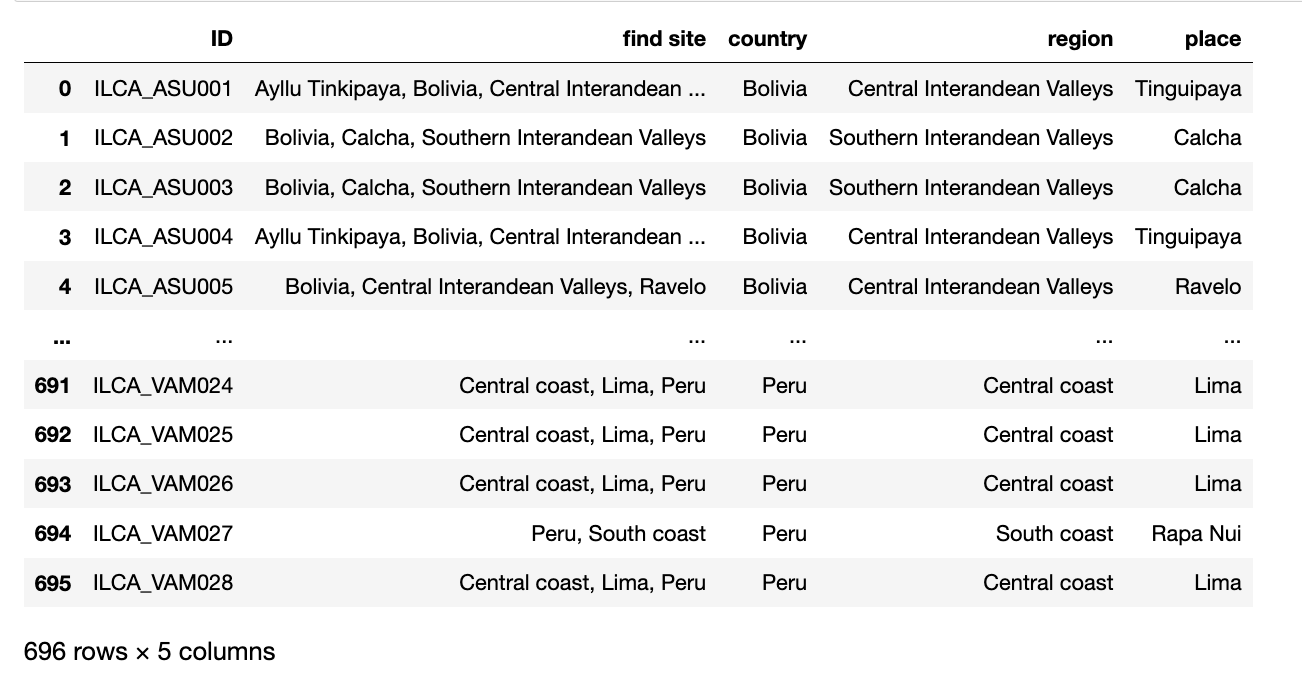
\includegraphics[width=11cm]{../images/geo_df_find.png}
           	 \caption{Tableau avec les trois niveaux de granularité séparés.}
           	 \label{fig:geo_df_find}
	 \end{center}
  \end{figure}
  
  \begin{figure}[!h]
    \begin{minipage}[c]{.5\linewidth}
            \begin{center}
                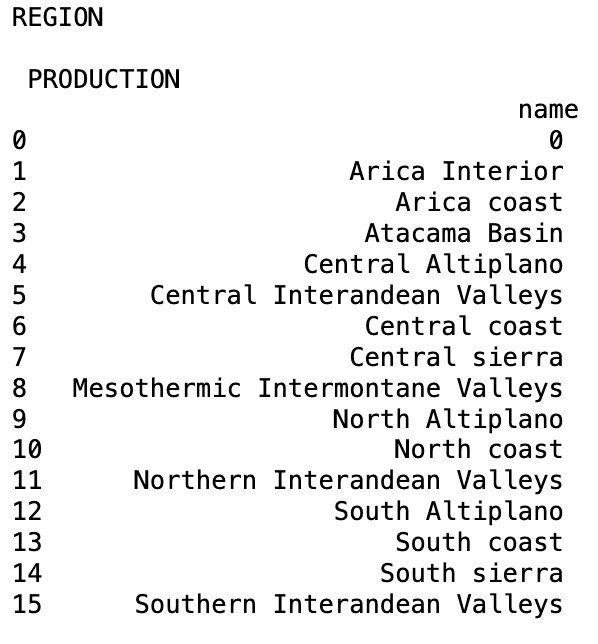
\includegraphics[width=5cm]{../images/regions_orig.png}
            \end{center}
            \caption{Régions originelles.}
            \label{fig:region_orig}   
    \end{minipage}
        \begin{minipage}[c]{.5\linewidth}
        \begin{center}
        		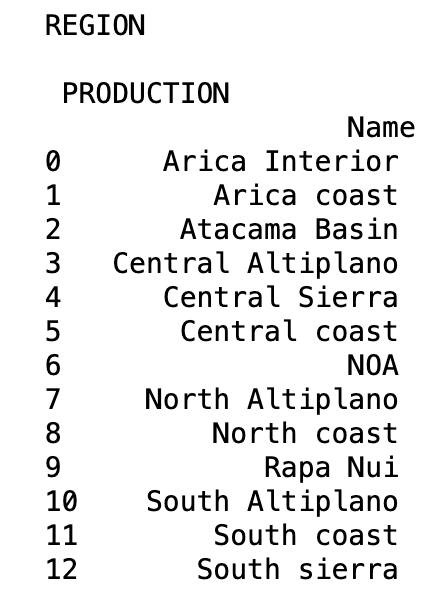
\includegraphics[width=4cm]{../images/regions_fin.png}
	\end{center}
	\caption{Régions finales.}
	\label{fig:region_fin}   
    \end{minipage}
\end{figure}
  
 Toutefois, les informations régionales -- qui sont les plus intéressantes puisque disponibles pour la plupart des textiles, avec une granularité plus importante que les pays -- ne sont pas standardisées et se recouvrent les unes les autres. À partir d'une première exploration, en localisant quelques noms de villages de la base de données dans Google Maps, nous observons cette superposition de certaines régions, comme le montre les images suivantes.
 
 \clearpage
 
   \begin{figure}[!h]
    \begin{minipage}[c]{.5\linewidth}
            \begin{center}
                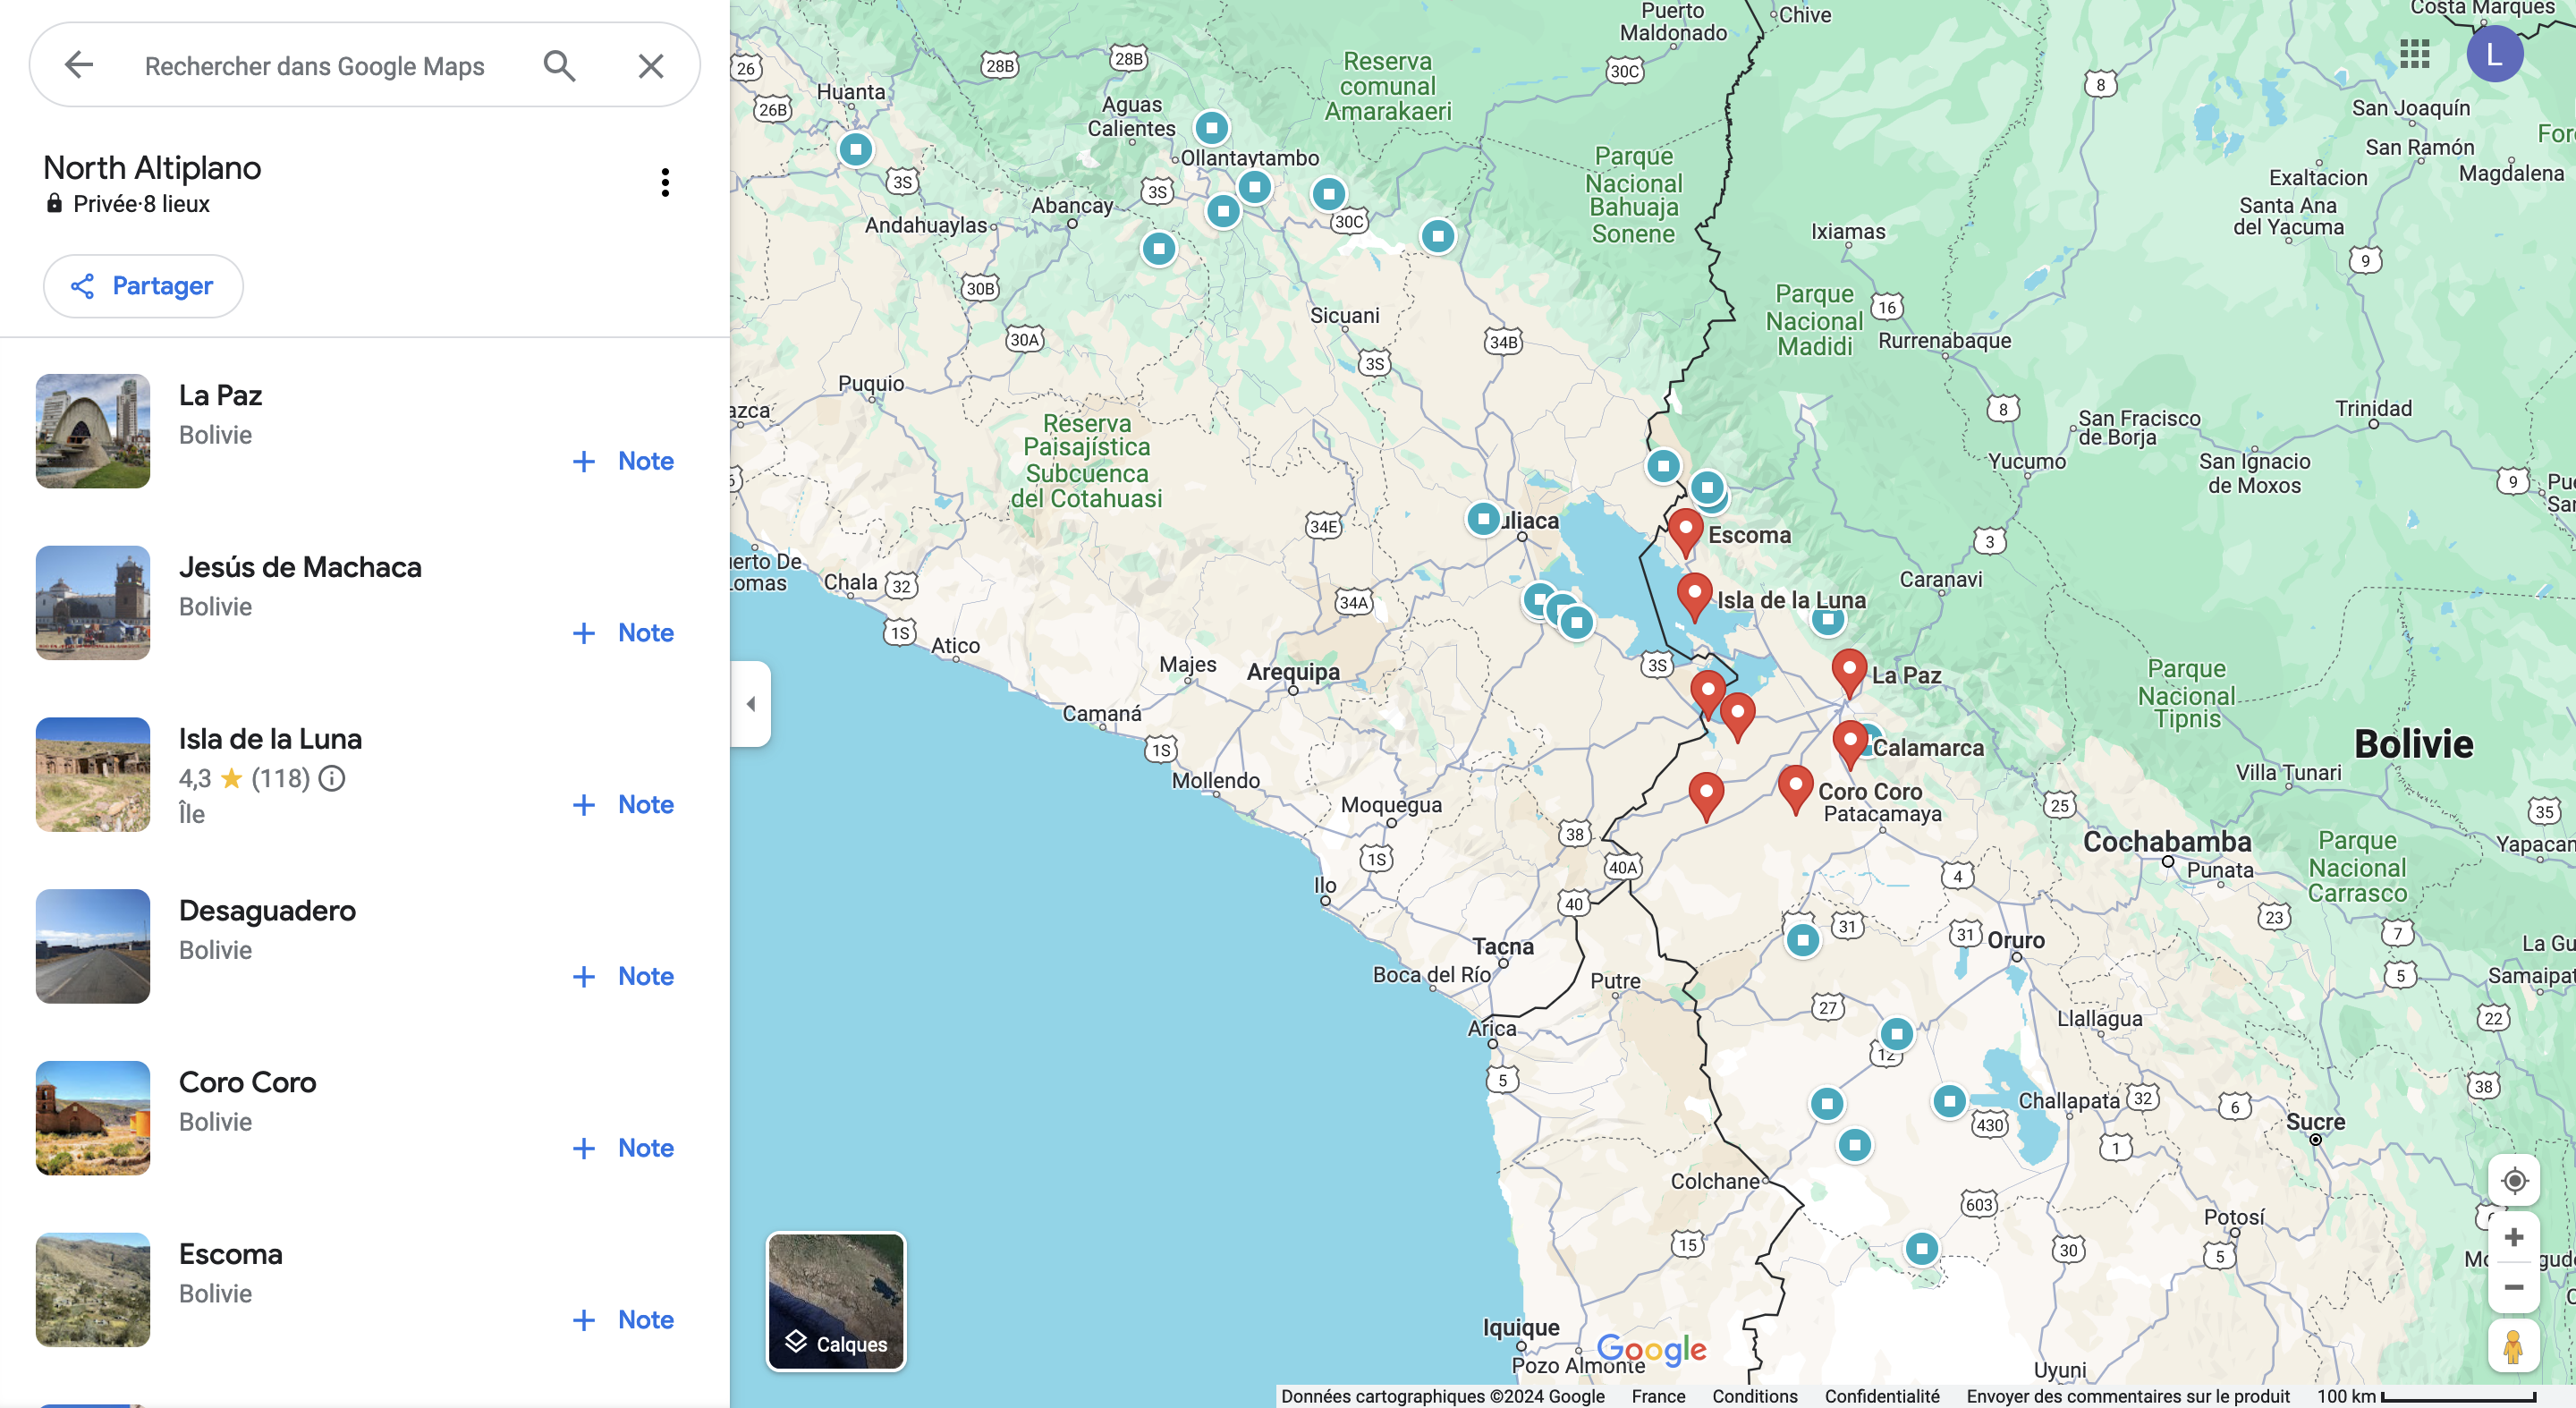
\includegraphics[width=8cm]{../images/GM_NorthAltiplano.png}
            \end{center}
    \end{minipage}
        \begin{minipage}[c]{.5\linewidth}
        \begin{center}
        		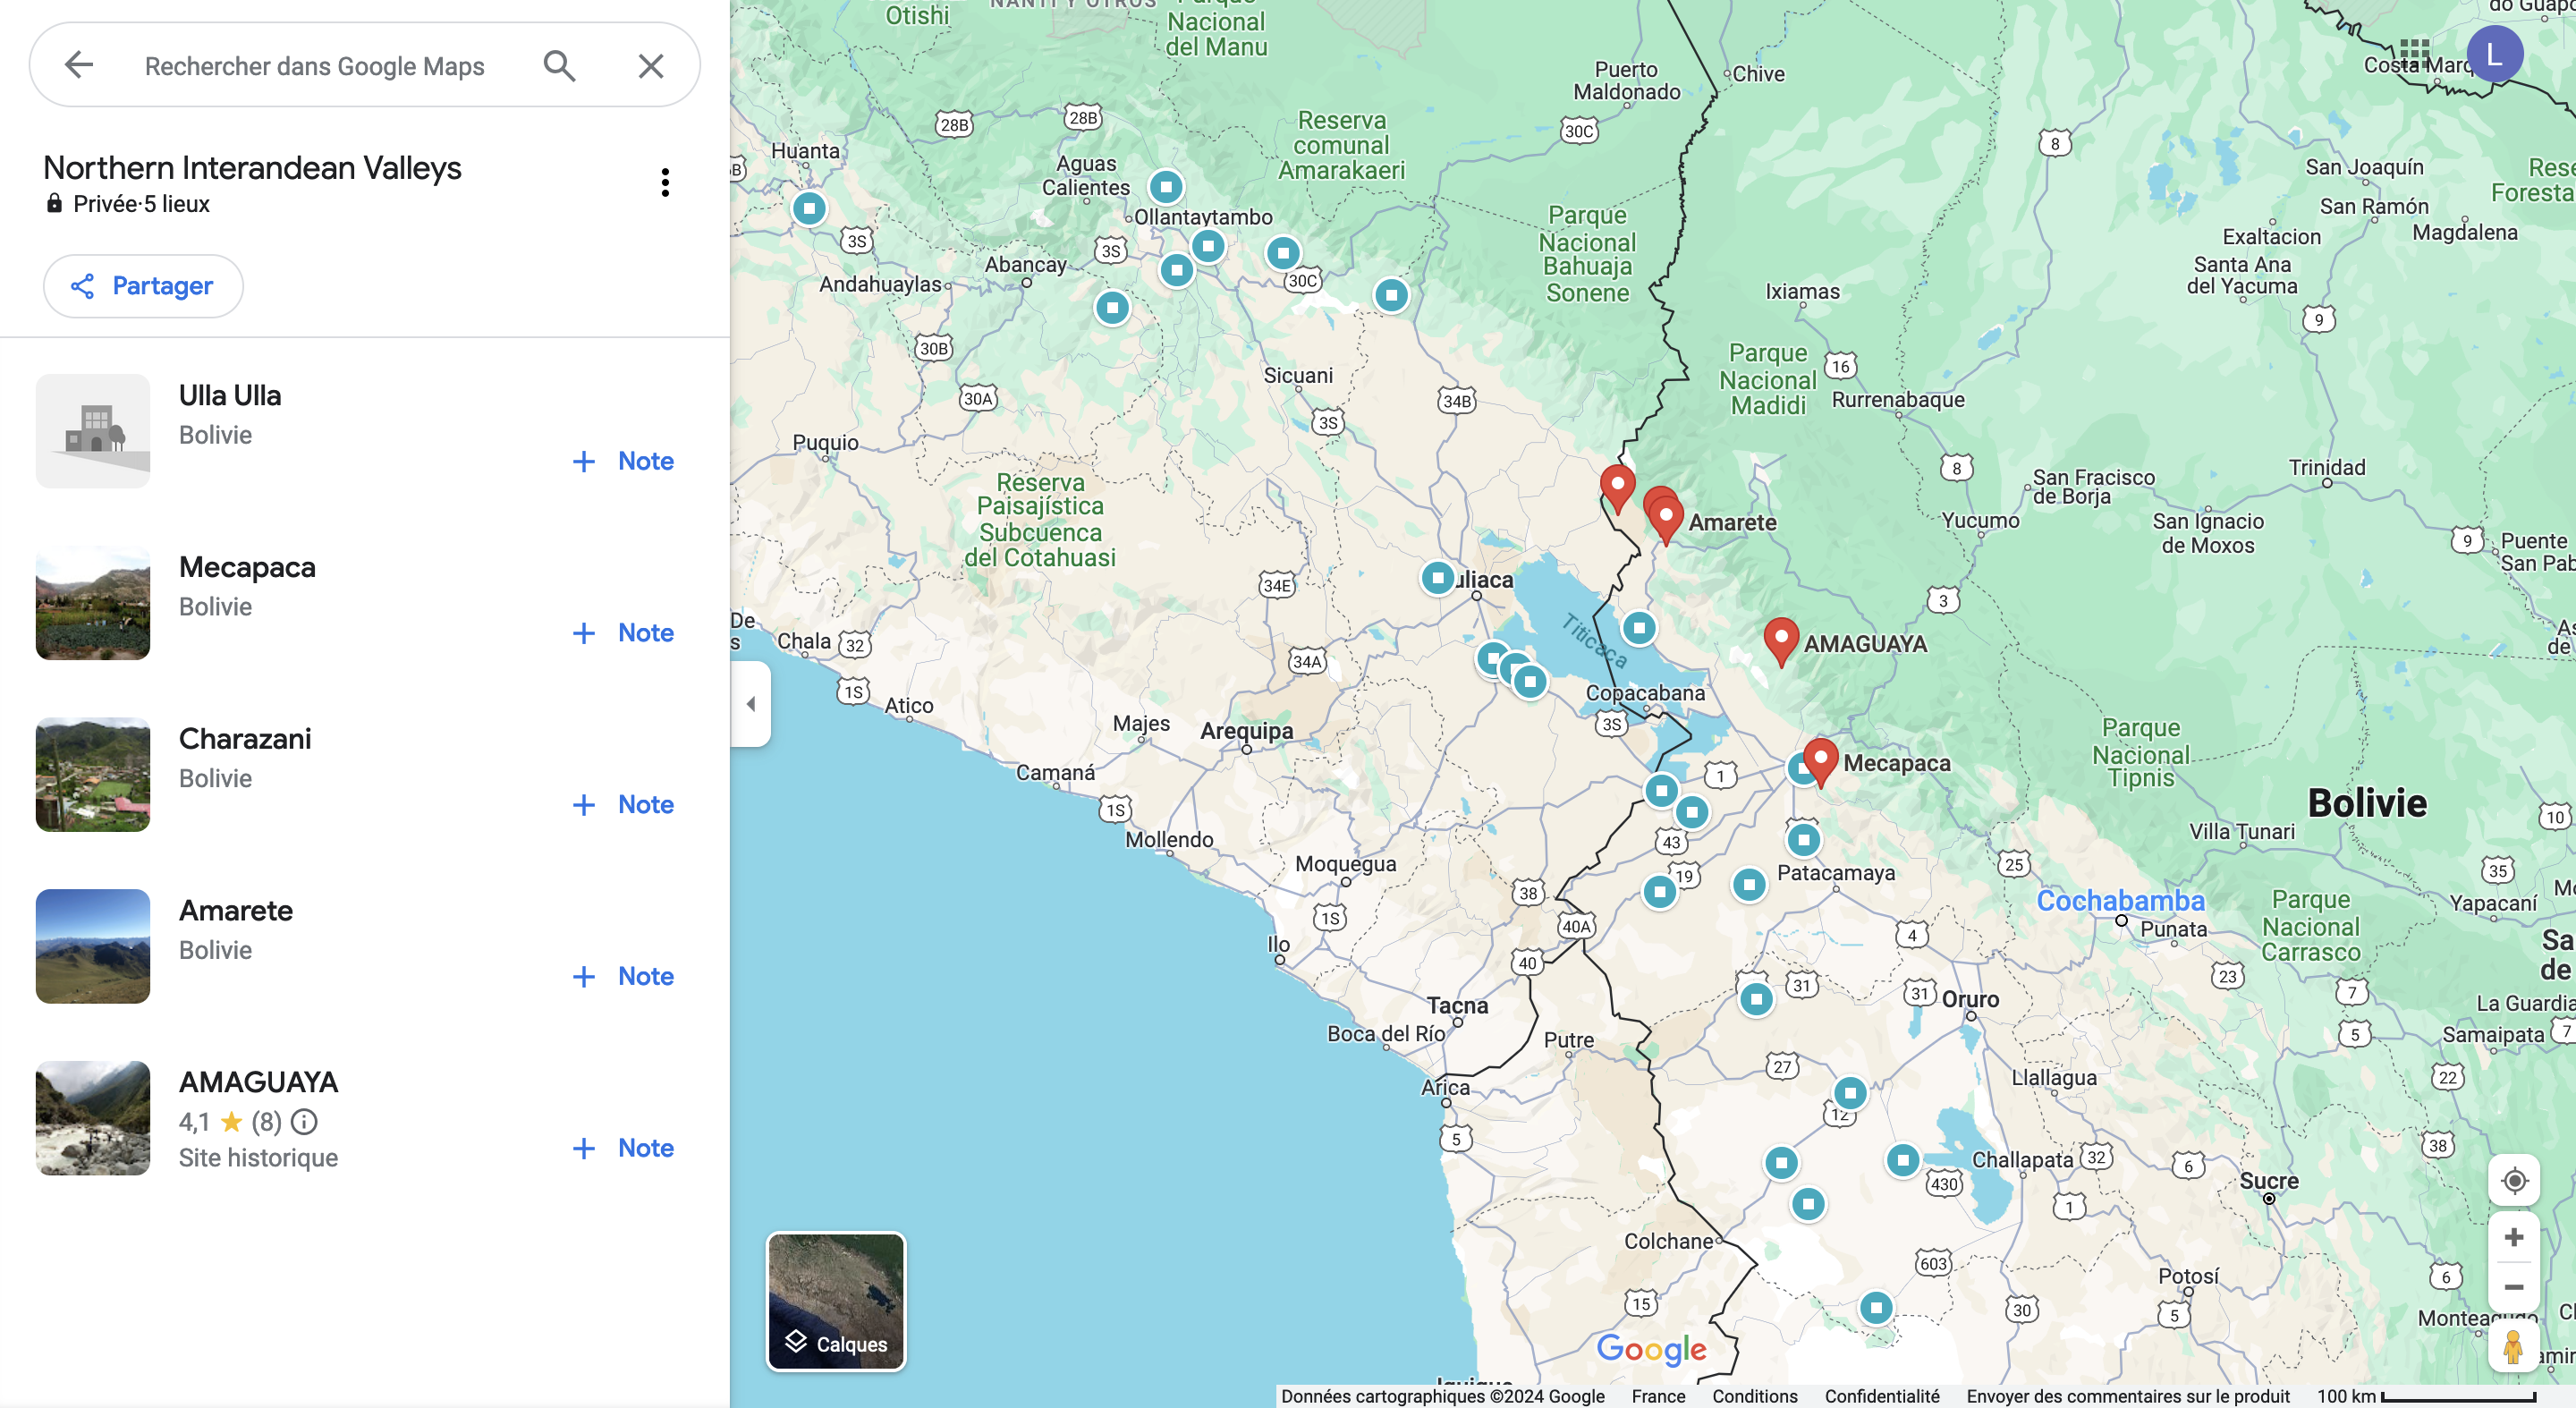
\includegraphics[width=8cm]{../images/GM_NorthernInterandeanValleys.png}
	\end{center}
    \end{minipage}
    	\caption{Captures d'écran de certains points des zones \og North Altiplano \fg \:et \og Northern Interandean Valleys \fg dans Google Maps.}
	\label{fig:GM}   
\end{figure}

Pour remédier à cela, nous avons fait le choix de réduire le nombre de régions de 15 à 12. Les régions qui contiennent le terme \og \textit{Interandean} \fg \:désignent les vallées à l'Est des hauts plateaux boliviens et péruviens (voir le tableau \ref{fig:region_orig}). Nous avons fait le choix de les associer aux zones équivalentes de l'Altiplano. Ce recoupage permet de récupérer des zones d'altitude unifiées d'une part et, d'autre part, des zones côtières. Pour les constituer nous nous sommes appuyés sur le travail de thèse de Romuald Housse en gardant la distinction entre zones péruviennes et boliviennes, présentes dans la base de données. 
 
  \begin{figure}[!h]
	\begin{center}
		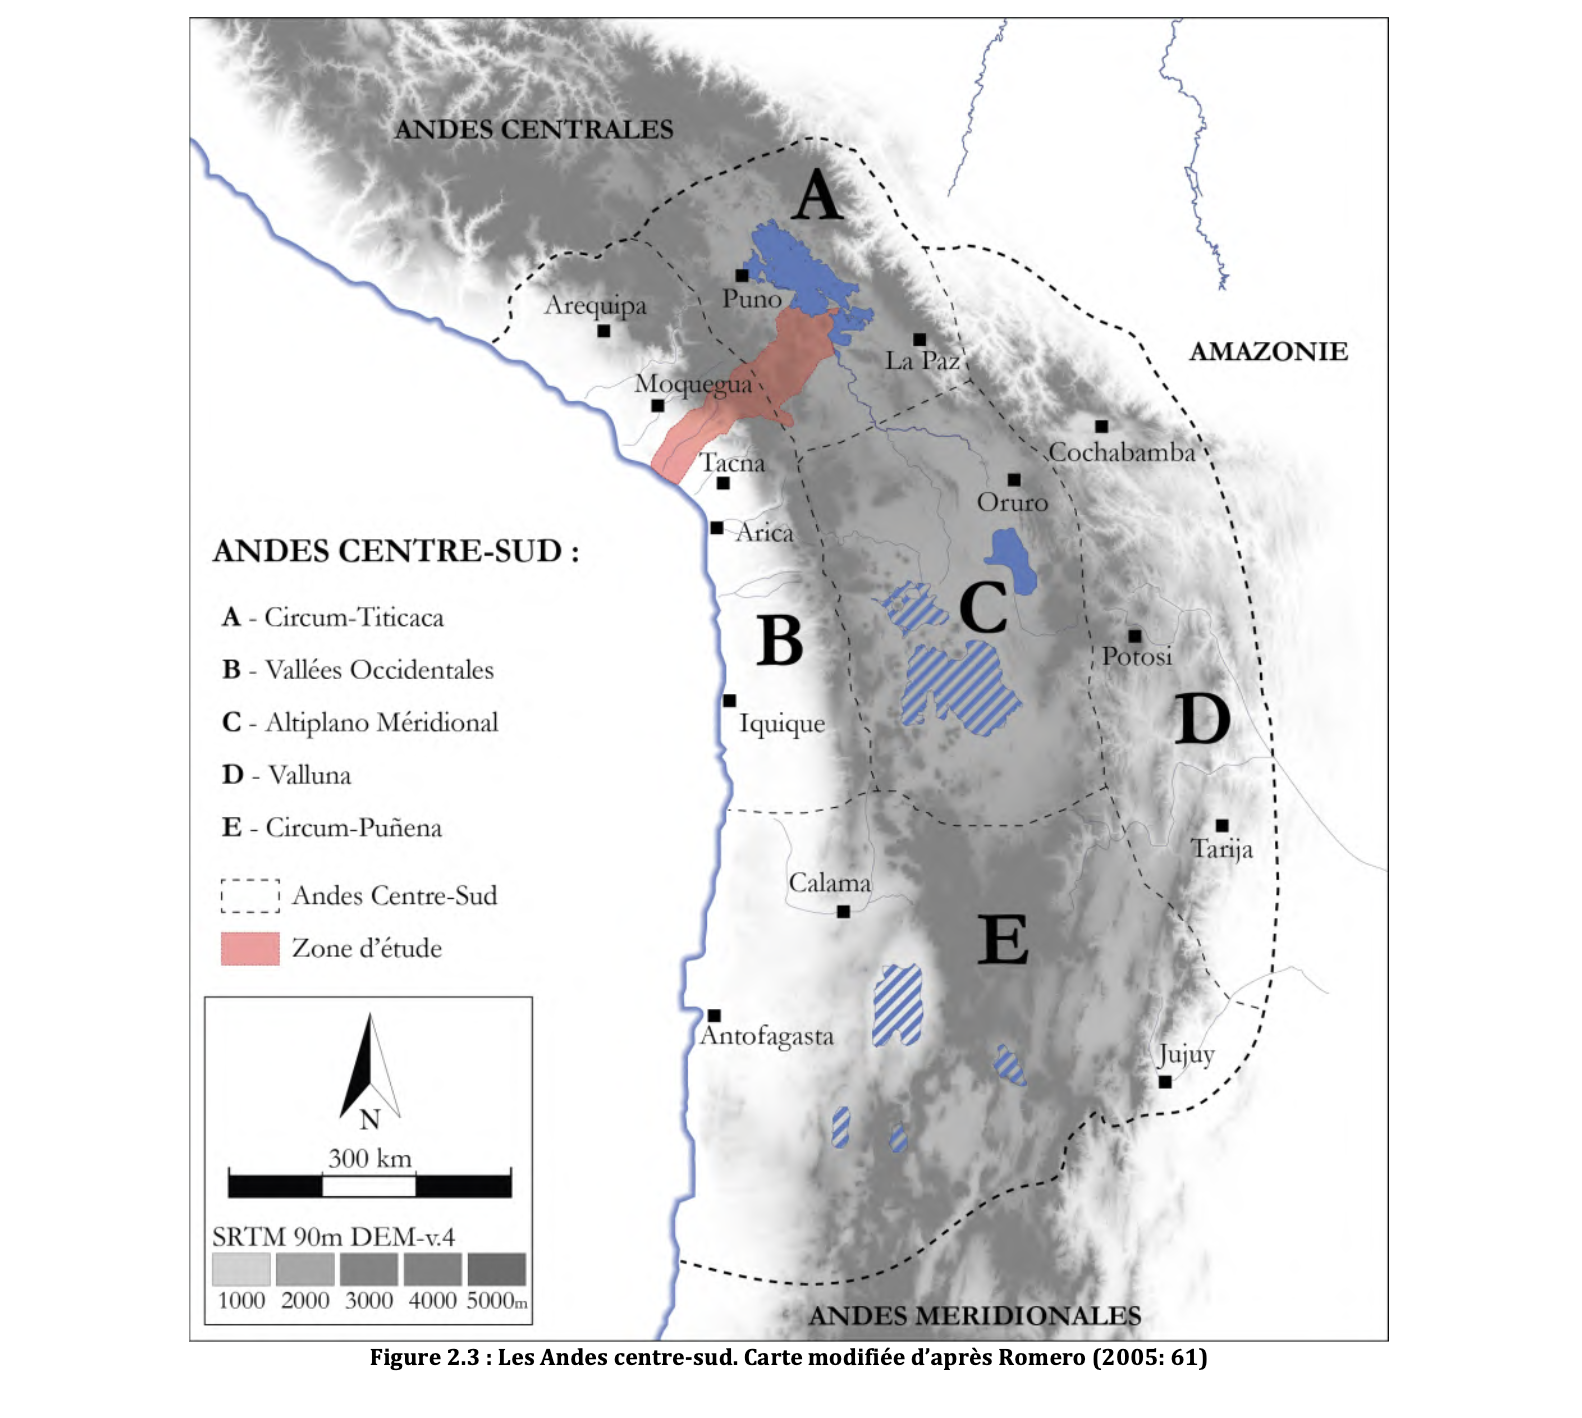
\includegraphics[width=10cm]{../images/mapHOUSSE_2021_p105.png}
           	 \caption{Carte des Andes centre-sud. \\ Source : Housse, 2021, p.~105.}
           	 \label{fig:carteHousse}
	 \end{center}
  \end{figure}

\noindent On obtient les \textbf{régions d'altitudes} suivantes, auxquelles s'ajoutent les régions côtières : 
\begin{itemize}
	\item South sierra (Pérou) : d'Ayacucho au lac Titicaca (inclut les îles péruviennes).
	\item Northern Interandean Valleys + \textbf{North Altiplano} : du lac Titicaca bolivien au nord d'Oruro.
	\item Central Interandean Valleys + \textbf{Central Altiplano} : Altiplano Méridional chez R. Housse, entre Oruro et le lac Poopo.
	\item Southern Interandean Valleys + \textbf{South Altiplano} : Circum-Puñena chez R. Housse mais sans la côte.
\end{itemize}

Après avoir standardisé les régions dans le tableur qui contient les informations de la base de données, nous avons eu recours au logiciel QGIS (logiciel de Système d'Information Géographique libre) pour dessiner et géo-localiser les régions\footnote{Le fichier shapefile contenant les géométrie des régions ainsi que leur localisation se nomme WCP\_region3.shp.}. Nous pouvons observer les régions finales, ainsi que leurs noms, sur la carte suivante.

  \begin{figure}[!h]
	\begin{center}
		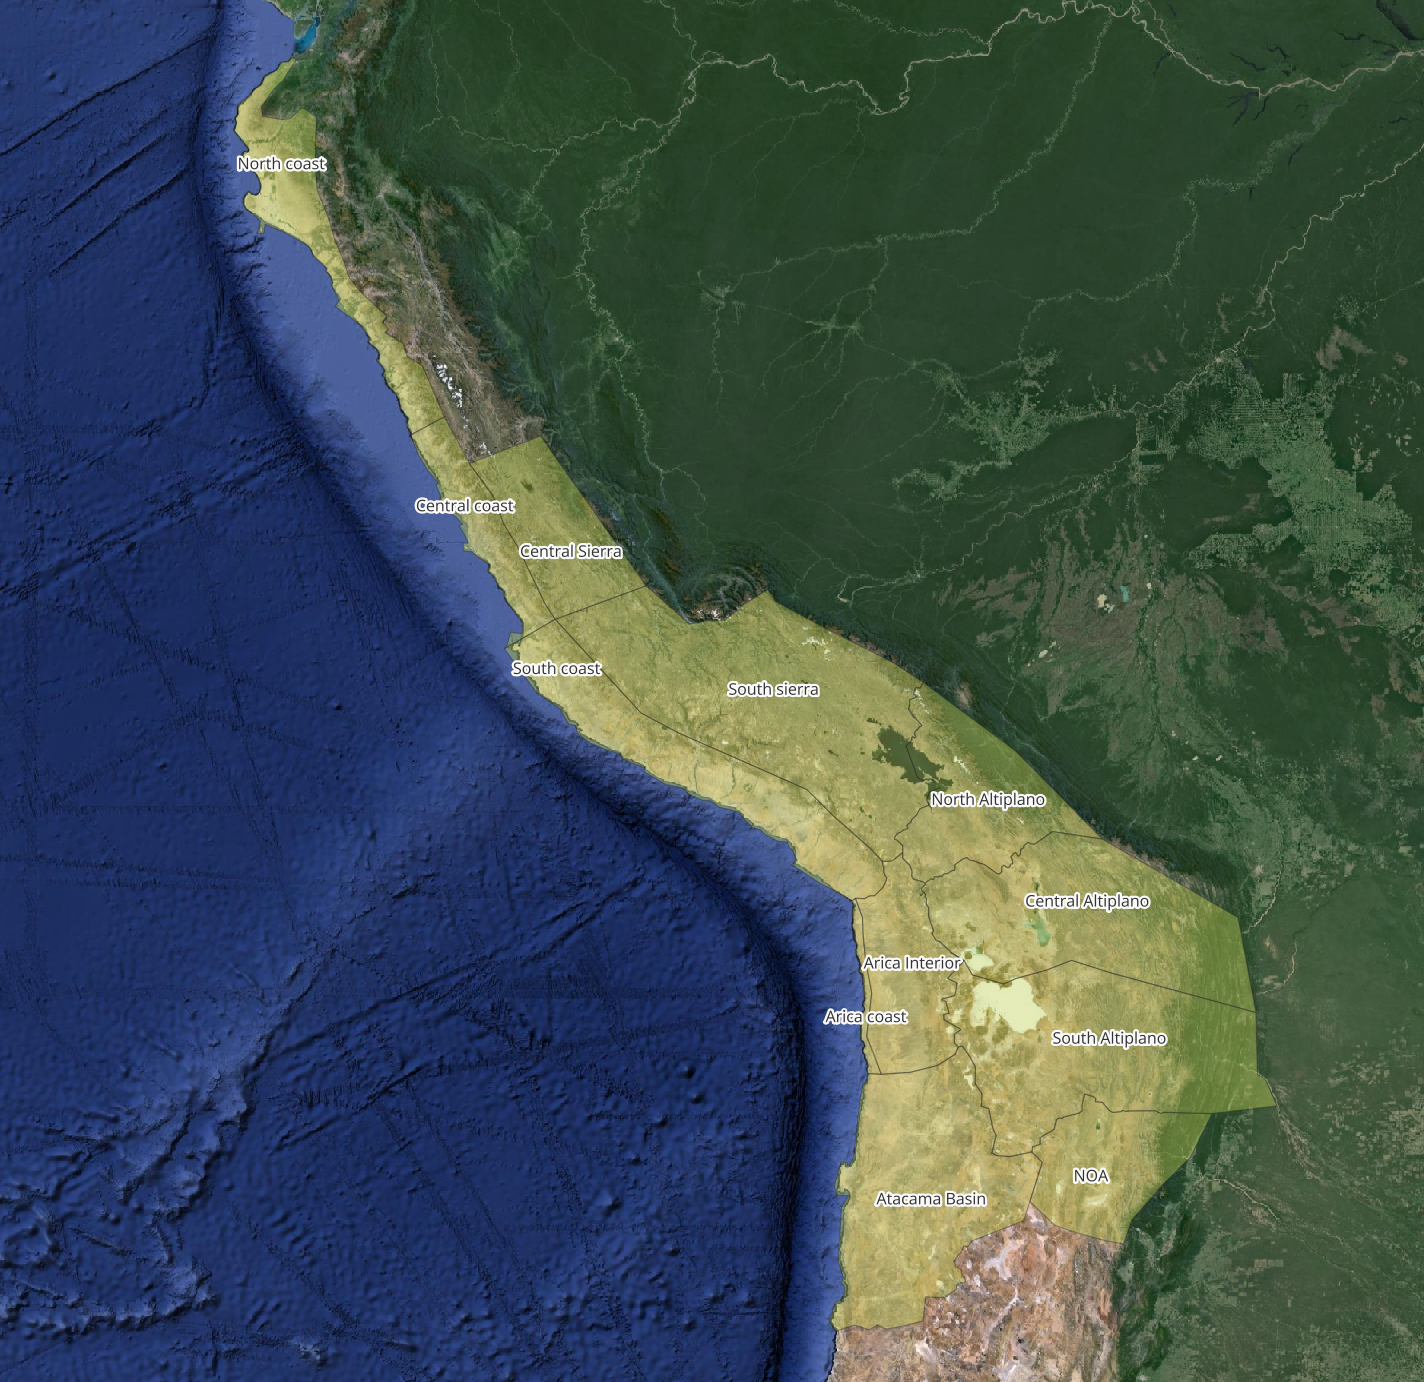
\includegraphics[width=15cm]{../images/region_fin.png}
           	 \caption{Carte des régions finales.}
           	 \label{fig:region}
	 \end{center}
  \end{figure}






\subsection{Premières analyses compréhensives des données}
Après la première phase de pré-traitement et avant de commencer tout travail d'analyse des données, une analyse exploratoire du corpus est nécessaire. À partir de l'ontologie, on peut récupérer les statistiques de chaque valeur dans chaque catégorie et ainsi leur répartition dans la base de données.

Dans le cas des catégories \og repository\fg \:et \og period\fg, c'est-à-dire les lieux de conservation des pièces et les périodes associées à chaque artefact, nous pouvons relever un certain déséquilibre. 
\noindent Les pièces sont réparties entre trois musées principaux : l'\textit{Instituto de Lengua y Cultura Aymara} (La Paz, Bolivie), le \textit{British Museum} (Londres, Royaume-Uni) et le \textit{Museo Nacional de Etnografía y Folklore} (La Paz, Bolivie). La première institution représente plus d'un tiers des pièces disponibles dans la base de données. Cette prépondérance s'explique par la spécificité de l'ILCA, institution partenaire du programme de recherche, dont la collection contient uniquement des textiles ethnographiques et des maquettes de motifs (voir \ref{fig:museum_period}), sa collection contient près de 70\% des textiles de la période républicaine (entre 1825 et aujourd'hui).

\begin{figure}[!h]
            \begin{center}
                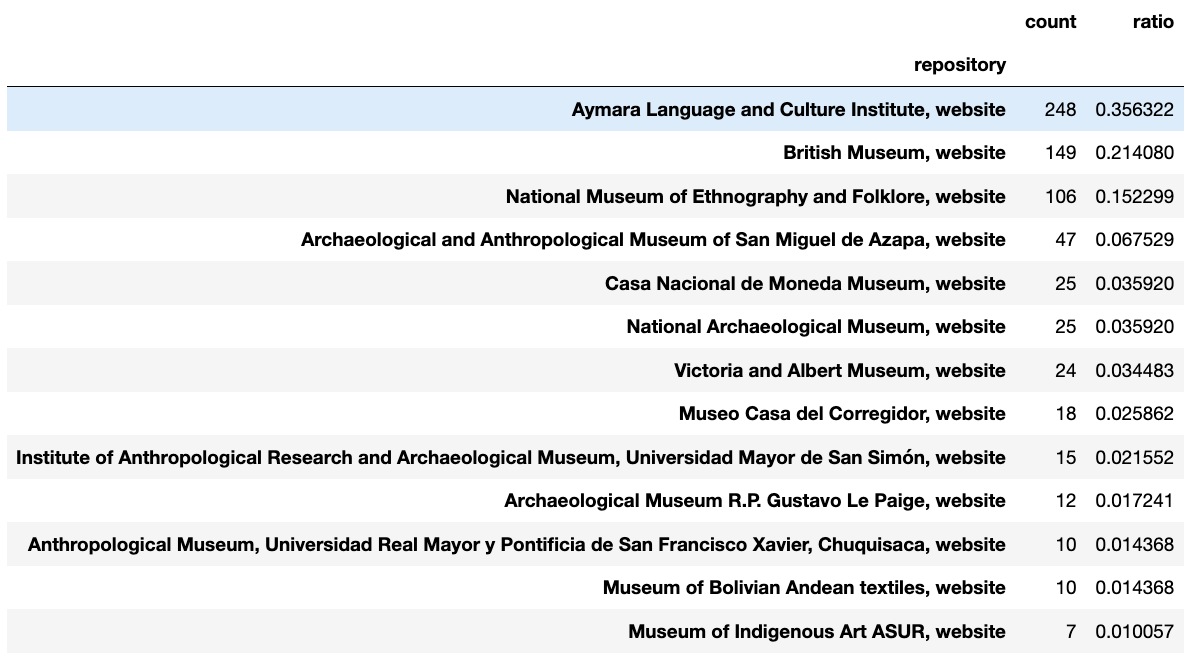
\includegraphics[width=12cm]{../images/count_repository.png}
            \end{center}
    \caption{Décompte des valeurs prises par la catégorie \og repository\fg}     
\end{figure}

\begin{figure}[!h]
        \begin{center}
        		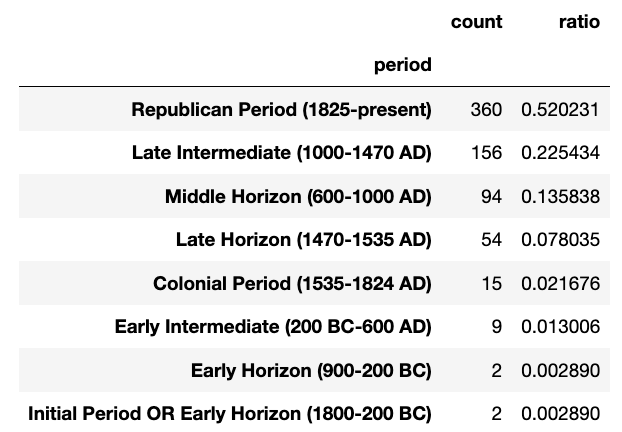
\includegraphics[width=8cm]{../images/count_period}
	\end{center}
    \caption{Décompte des valeurs prises par la catégorie \og period\fg}     
    \label{fig:period}
\end{figure}

Dans le cas de la datation des pièces textiles, la répartition inégale entre les périodes est principalement le fait du choix des experts et des collections auxquelles ils avaient accès. Nous pouvons cependant relever que le nombre de données diminue avec l'ancienneté. La plupart des pièces sont postérieures à la colonisation (375 pièces), et les pièces antérieures se concentrent entre l'Horizon Moyen, la période Intermédiaire Récente et l'Horizon Récent (304 pièces). L'échantillon de textiles disponibles est donc relativement équilibré entre pièces archéologiques d'un côté et pièces historiques et contemporaines de l'autre. Toutefois, plus de 50\% des pièces appartiennent à la période républicaine. Cette prépondérance s'explique notamment par les processus naturels de destruction des textiles. Les périodes les plus anciennes sont ainsi les périodes qui fournissent le moins de textiles.
Dans le cas de la période coloniale et de l'Horizon Récent, plusieurs hypothèses (autre que la sélection réalisée par les chercheurs et chercheuses) peuvent expliquer le nombre plus faible de textiles disponibles. La Conquête (soit la fin de l'Horizon Récent et le début de la période coloniale) est marquée par de nombreux affrontements : les chroniqueurs relatent la destruction volontaire des entrepôts de textiles par les armées incas qui se retiraient devant l'ennemi pour limiter son avancée. Ainsi, John Murra indique que \og L'ennemi [espagnol] n'était pas privé d'hommes (qui, selon Garcilaso, joignaient l'armée européenne) ou de lamas, mais de tissus\footnote{\cite[p.~718]{murraClothItsFunctions1962}. Texte original : \textquotedblleft \textit{The enemy was not deprived of the men (who, according to Garcilaso, joined the European army) or of llamas, but of cloth.}\textquotedblright}.\fg \:Ces témoignages expliquent une partie de la disparition des pièces textiles de cette période, même si une grande quantité de pièces a survécu et se trouve dans les collections de musées qui n'appartiennent pas à notre base de données\footnote{Par exemple, le musée du textile précolombien Amano (Lima), le musée Inka (Cuzco), le musée Larco (Lima)...}. Suite à la Conquête, les espagnols implantent les \textit{obrajes} et développent un nouveau système de production textile pour les populations indigènes. L'apparition de ces manufactures textiles et les différentes lois de la métropole espagnole interdisant certaines pratiques vestimentaires n'impliquent pas la disparition des pratiques textiles pré-coloniales\footnote{\cite[par.~3] {desrosiersLogicasTextilesLogicas1997}}. Cependant, n'étant plus intégrés aux pratiques de l'élite, les textiles perdent de leur attrait pour les scientifiques européens et sont donc plus rarement conservés. L'intérêt pour ces textiles reprend au \siecle{xxi} c'est-à-dire à la période républicaine dans notre chronologie. Par ailleurs, les textiles sélectionnés pour la base de données sont des textiles andins, catégorie qui ne prend pas en compte les textiles produits en grande quantité dans les \textit{obrajes}. 
D'après ce que nous savons, il n'existe pas d'enquête statistique exhaustive sur la quantité de textiles archéologiques disponibles pour la région andine. Techniquement, ces variations dans la répartition posent problème. En effet, les méthodes d'intelligence artificielle nécessitent des corpus d'entraînement équilibrés, avec le même nombre d'éléments par classe (ici, par période), sinon les algorithmes ont tendance à sur-classifier dans les classes prépondérantes de l'échantillon.

 \begin{figure}[!h]
        \begin{center}
        		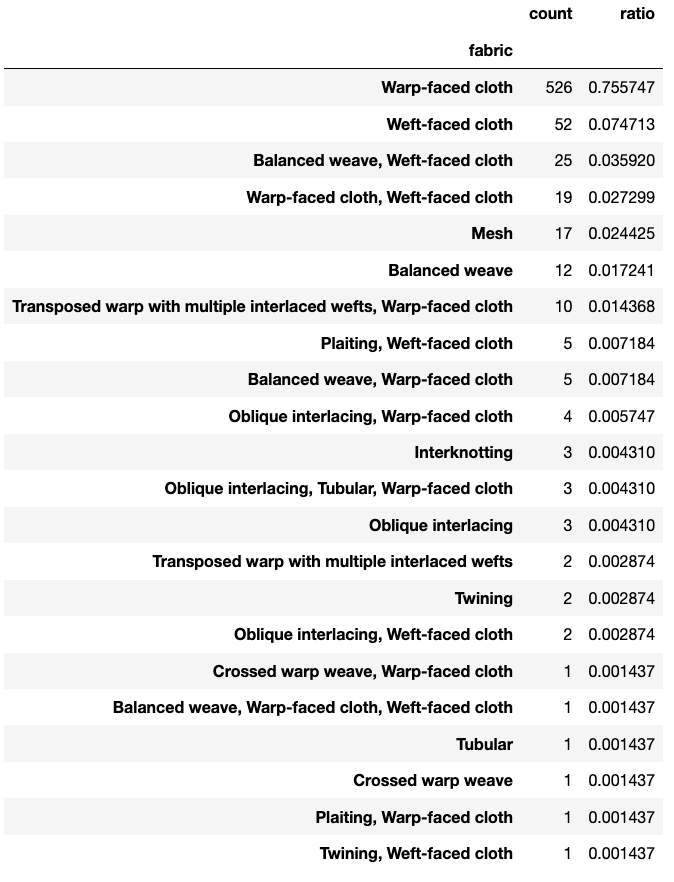
\includegraphics[width=9cm]{../images/count_fabric.png}
	\end{center}
    \caption{Décompte des valeurs prises par la catégorie \og fabric\fg}     
    \label{fig:fabric}
\end{figure}

\clearpage

Nous pouvons aussi nous intéresser aux caractéristiques techniques des pièces textiles. La base de données contient la plupart des structures textiles découvertes dans les Andes\footnote{Voir \cite{harcourtTextilesAnciensPerou2008}.} : toile (\textit{balanced weave}), tissage face chaîne (\textit{warp-faced cloth}), tissage face trame ou tapisserie (\textit{weft-faced cloth}), double étoffe (\textit{double cloth} ou \textit{twining}), réseau (en mailles, \textit{mesh}, ou noué, \textit{interknotting}) et tresse (\textit{plaiting}). 
Là aussi la base de données est déséquilibrée, les tissages face chaîne sont sur-représentés, composant 75,57\% du corpus. Cette sur-représentation va de pair avec la prédominance des pièces contemporaines. Ces textiles contemporains viennent en effet principalement des hautes-terres (voir \ref{fig:place_period}) où le tissage à face chaîne est dominant, et ce sur la longue durée. \\

Ces tableaux nous permettent donc d'obtenir la répartition des métadonnées textiles\footnote{Le reste des tableaux disponibles se trouve en annexe.}. Nous avons ainsi une idée des valeurs disponibles pour chaque catégorie mais il est aussi important de se questionner sur l'influence mutuelle de ces catégories. Pour cela, nous pouvons représenter graphiquement les variables les unes par rapport aux autres afin de voir si des tendances apparaissent. Ces représentations graphiques sont fonctionnelles uniquement pour les catégories qui ont un nombre de valeurs raisonnables. 
Nous analysons ci-dessous plusieurs cas intéressants, soit parce qu'ils illustrent un trait caractéristique de notre \textit{dataset} ou bien parce qu'ils concernent les données que nous mobiliserons dans la suite de ce travail.

 
 \begin{figure}[!h]
	\begin{center}
		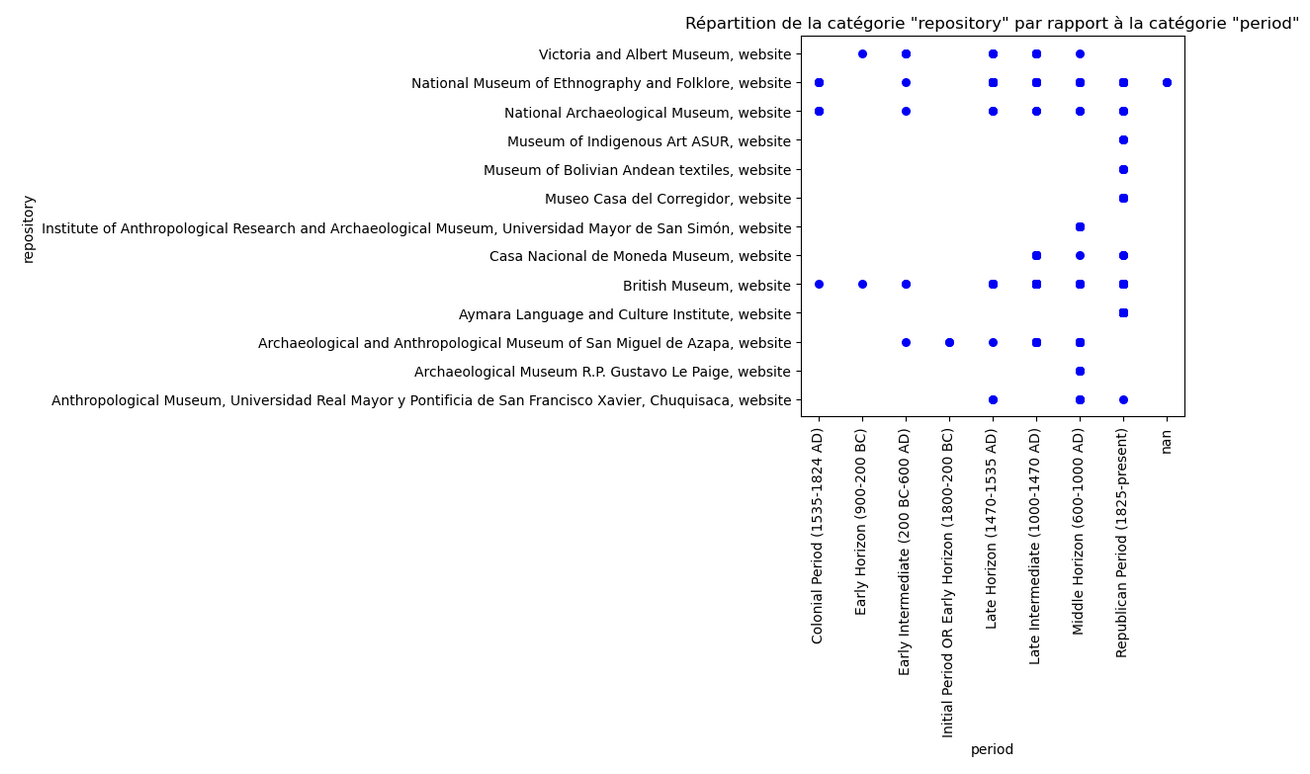
\includegraphics[width=16cm]{../images/R_period_repository.png}
		\caption{Répartition des valeurs possibles prises par es pièces textiles pour les catégories musées et périodes}
		\label{fig:museum_period}
	 \end{center}
\end{figure}

Cette analyse est particulièrement éclairante pour comprendre comment les textiles sont répartis entre les différents musées.  Comme nous l'avons vu la collection issue de l'\textit{Instituto de Lengua y Cultura Aymara} contient uniquement des pièces récentes (période républicaine). Il en est de même pour le \textit{Museo de Arte Indigena} (Sucre, Bolivie), le \textit{Museo de Textiles Andinos Bolivianos} (La Paz, Bolivie) et le \textit{Museo Casa del Corregidor} (Puno, Pérou) qui détiennent des petites collections. À l'inverse, le \textit{Victoria and Albert Museum} (Londres, Royaume-Uni), l'\textit{Instituto de Investigaciones Antropológicas y Museo Arqueológico} (Cochabamba, Bolivie), le \textit{Museo Arqueológico R. P. Gustavo Le Paige} (San Pedro de Atacama, Chili) et le \textit{Museo Arqueologico San Miguel de Azapa} (San Miguel de Azapa, Chili) ont des collections uniquement pré-hispaniques.

\begin{figure}[!h]
    \begin{minipage}[c]{.5\linewidth}
            \begin{center}
                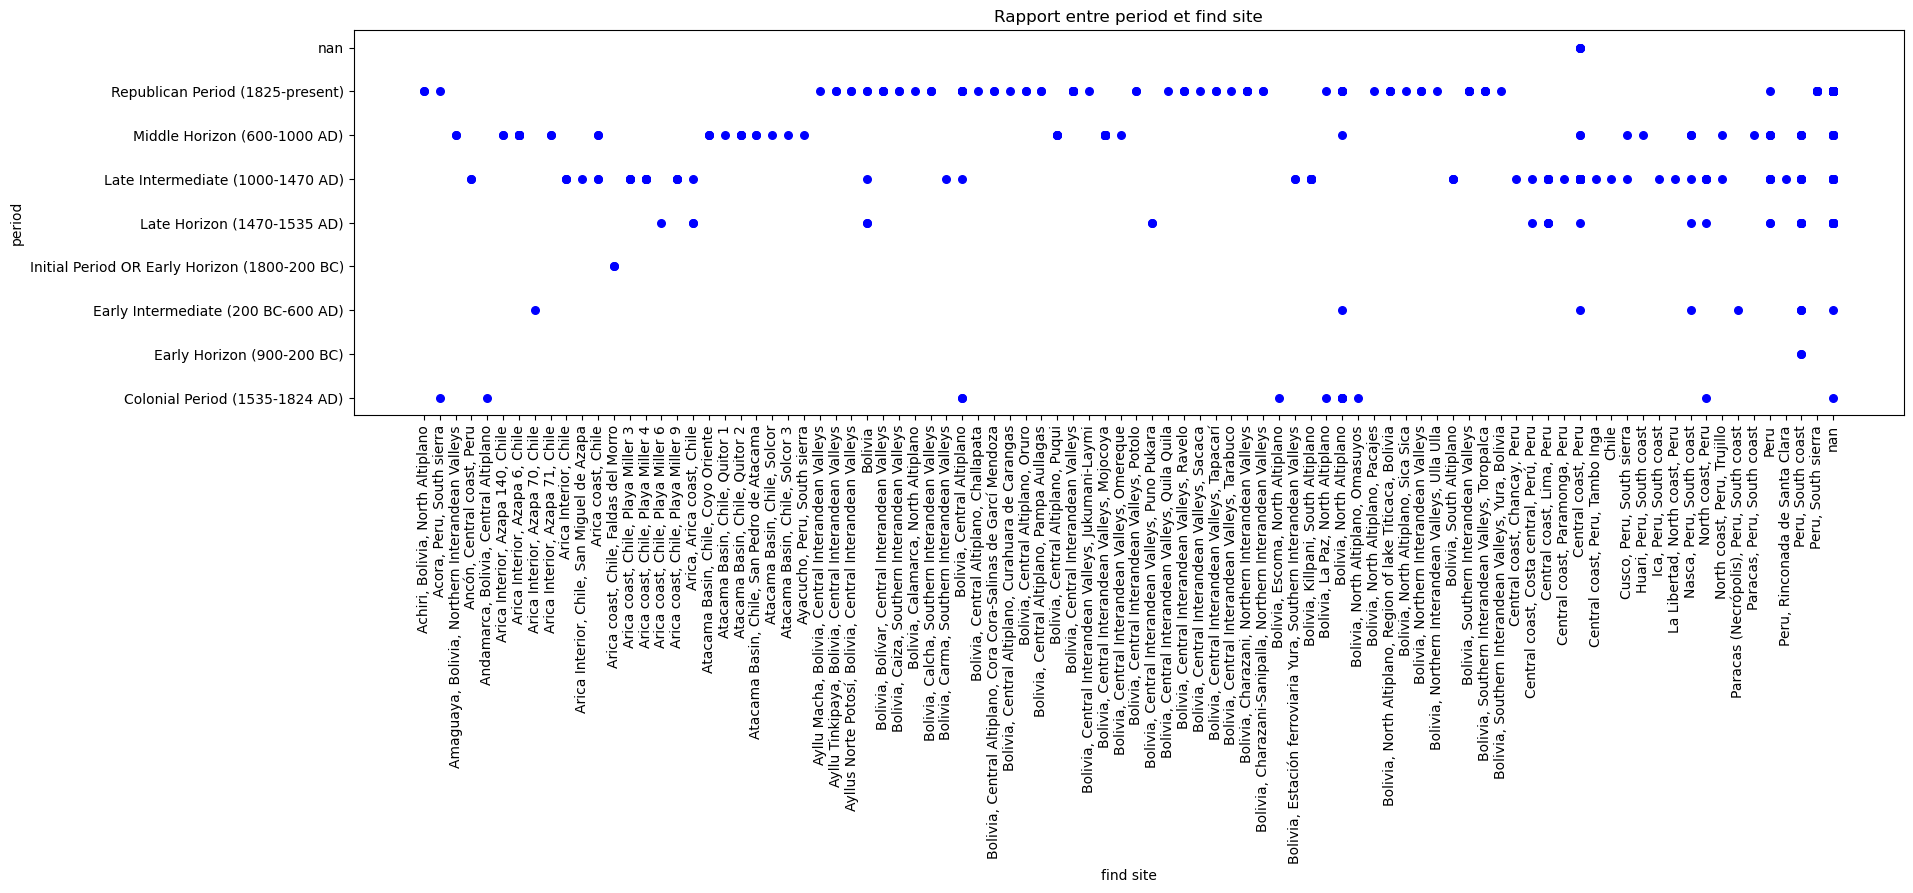
\includegraphics[height=8cm, angle=-90]{../images/R_period_find_site.png}
            \end{center}
    \end{minipage}
        \begin{minipage}[c]{.5\linewidth}
        \begin{center}
        		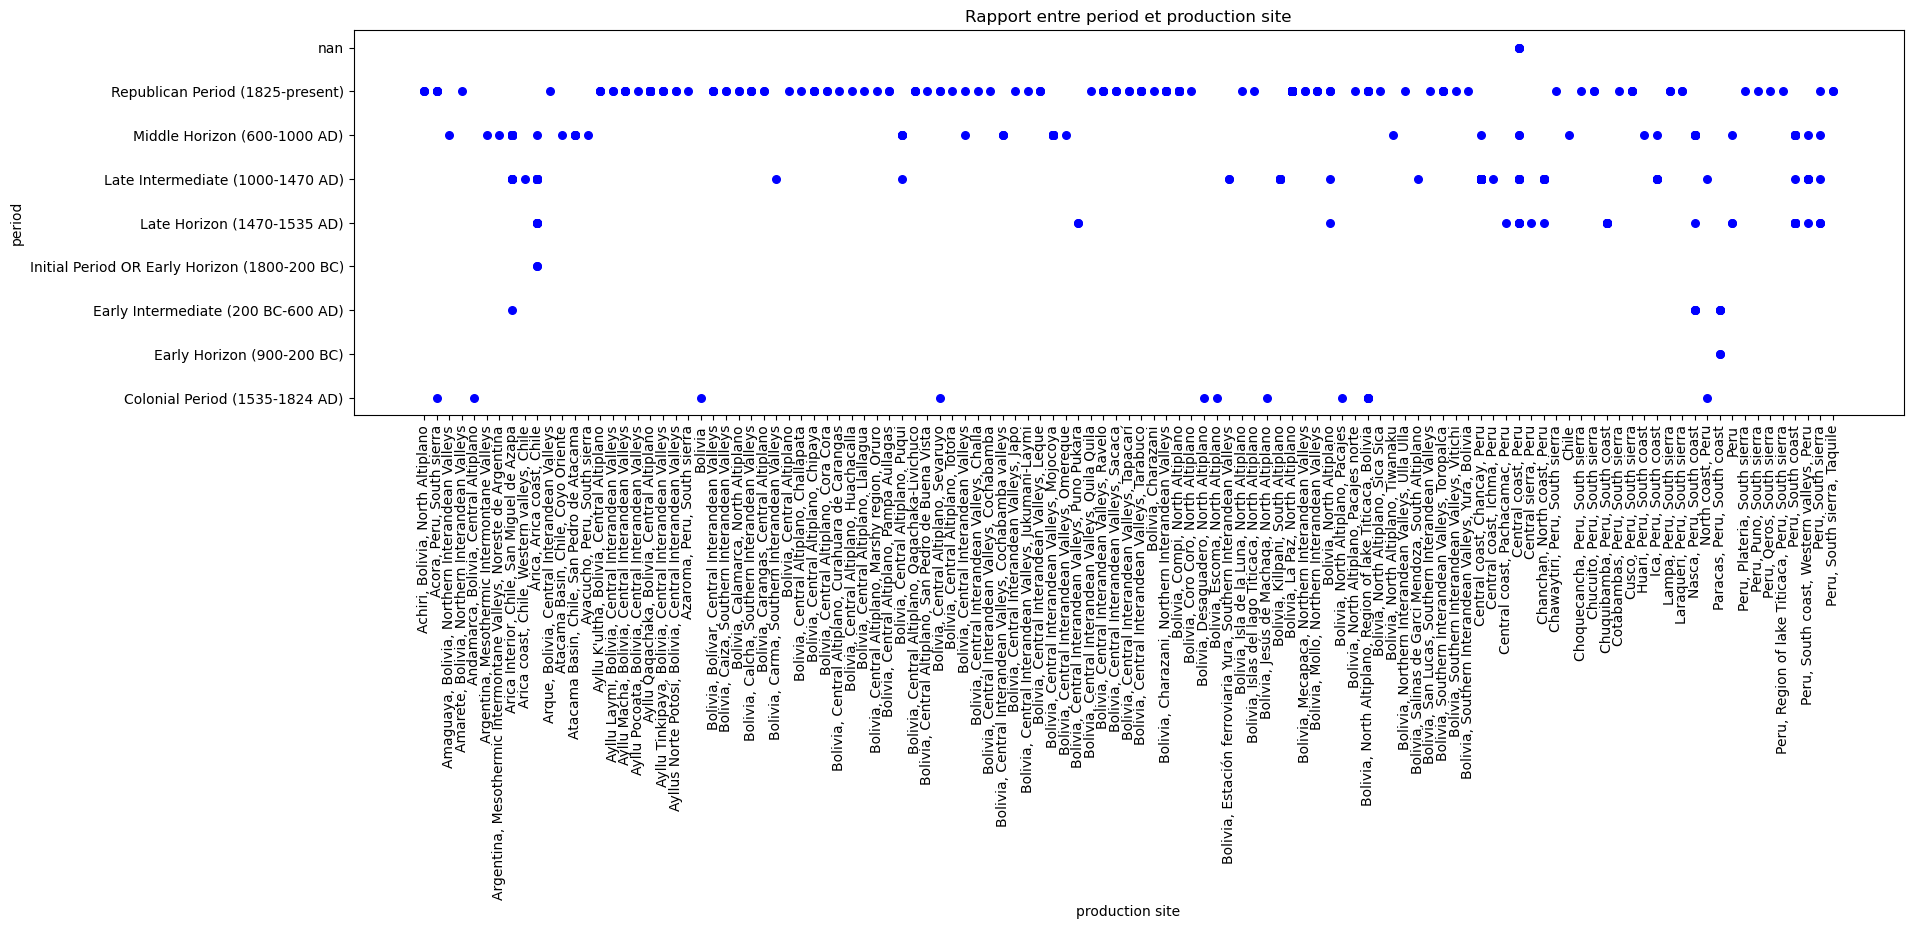
\includegraphics[height=8cm, angle=-90]{../images/R_period_production_site.png}
	\end{center}
    \end{minipage}
    \caption{Répartition des valeurs possibles prises par les pièces textiles pour les catégories période, lieux de découverte et lieux de production}
    \label{fig:place_period}   
\end{figure}
  
À partir du schéma de la répartition des valeurs prises par les pièces textiles pour les catégories périodes et lieux de découverte, nous pouvons observer que la majeure partie des pièces textiles appartiennent aux périodes archéologiques de l'Horizon Moyen (600-1000), de la période intermédiaire tardive (1000-1470) et la période républicaine (1825 - aujourd'hui). Les \textit{clusters} qui se forment sur le graphique nous indiquent la répartition géographique des textiles par période. Ainsi, les textiles de la base de données provenant d'Arica ont été produits sur toutes les périodes exceptée la période contemporaine, la période coloniale et l'Horizon Ancien.
Ceux provenant du désert d'Atacama ont tous été produits au cours de l'Horizon Moyen. Les textiles de la côte centrale péruvienne sont principalement des pièces de l'Intermédiaire Récent et de l'Horizon Récent.
À l'inverse, les pièces contemporaines sont majoritairement issues de Bolivie. Ces répartitions s'expliquent notamment par le contexte de conservation archéologique déjà mentionné. Nous retrouvons quasiment les mêmes répartitions pour les lieux de production.

Ces deux graphiques l'un à côté de l'autre nous permettent de mieux saisir la différence entre les deux catégories géographiques. La catégorie\og lieu de découverte \fg \:indique les lieux d'excavation ou de récupération des pièces textiles, elle est donc composée de plus de textiles archéologiques.
La catégorie \og lieu de production \fg \:contient les informations de production des pièces textiles, c'est-à-dire l'endroit où le textile a été tissé. Il est donc cohérent que cette catégorie contienne plus de textiles contemporains qui sont des textiles qui ont été collectés dans le cadre de recherches ethnographiques bien souvent directement auprès de leur productrice ou de leur producteur.



\section{Traitement des données géographiques}
\subsection{Géocodage des informations géographiques de la base de données}

Après avoir pré-traité les chaînes de caractères des lieux de production et de découverte, nous leur attribuons des coordonnées géographiques, c'est-à-dire une longitude et une latitude\footcite[p.~34]{goldbergTextGeographicCoordinates2007}. Cette méthode de géocodage permet de construire un Système d'Informations Géographiques (ou SIG), c'est-à-dire un ensemble organisé de données spatiales et de données issues des sciences sociales. Nés dans le domaine de la géographie numérique, les SIG se diffusent dans les sciences sociales à partir des années 1970\footnote{\cite[par.~3]{brandoIntroductionHumanitesNumeriques2021}. Voir également le recensement de projets de SIG en histoire et archéologie suivant : \cite{abaranesBibliographieAnalyseSpatiale2021}.}. Aux cartographies se greffent alors les sources iconographiques et textuelles, complétant l'information spatiale.
La base de données contient des données géographiques récentes puisque les chercheurs  ont attribués des lieux contemporains aux textiles et non des lieux historiques. Le processus de géocodage peut donc avoir recours à une base de données géographiques contemporaines. 
Dans ce cas, nous avons eu recours à l'interface de programmation (API) d'Open Street Map, base de données géographique libre et collaborative (sur le modèle de Wikipédia). Nominatim, le géocodeur d'Open Street Map, peut être intégré dans un code en Python auquel on fournit une adresse (plus ou moins précise) et qui nous renvoie des coordonnées géographiques\footnote{Une partie du code utilisée à été extraite de ce tutoriel : visité le 15 décembre 2023, \url{https://medium.com/@amorrison_58444/geocoding-with-the-openstreetmap-api-and-geopy-325633980a15}.}. 

 \begin{figure}[!h]
	\begin{center}
		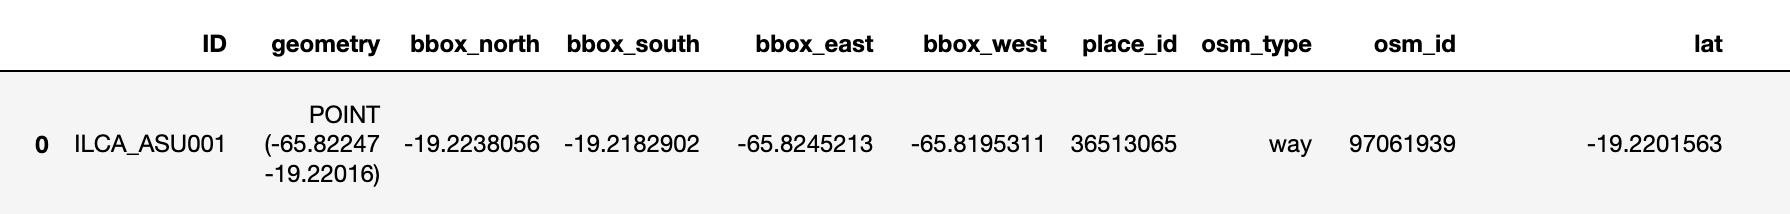
\includegraphics[width=15cm]{../images/gdf_places_prod.png}
	 \end{center}
\end{figure}
 \begin{figure}[!h]
	\begin{center}
		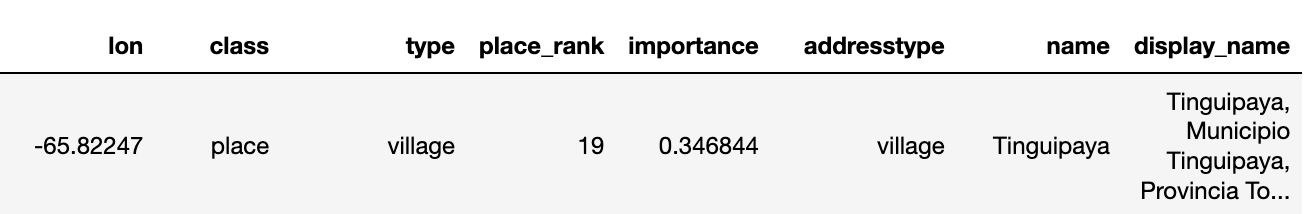
\includegraphics[width=12cm]{../images/gdf_places_prod2.png}
	 \end{center}
	 \caption{Tableau final contenant les identifiants des textiles et les résultats du géocodage.}
	 \label{fig:gdf_places_prod}
\end{figure}

Pour la base de données, les informations géographiques n'étant pas des adresses précises (avec un nom et un numéro de rue), Nominatim nous renvoie plutôt des polygones -- couvrant un périmètre -- que des points précis. Afin de récupérer une latitude et une longitude pour chaque élément, nous récupérons donc le centroïde de chaque polygone et créons une géométrie \og point \fg \:contenant les informations de longitude et de latitude pour chaque textile. Nous réalisons ce processus pour les lieux de production et pour les lieux de découverte. Cette simplification est nécessaire mais pose certains questionnements puisqu'elle implique une perte de précision.

\begin{wrapfigure}{r}{0.4\textwidth}
    \centering
    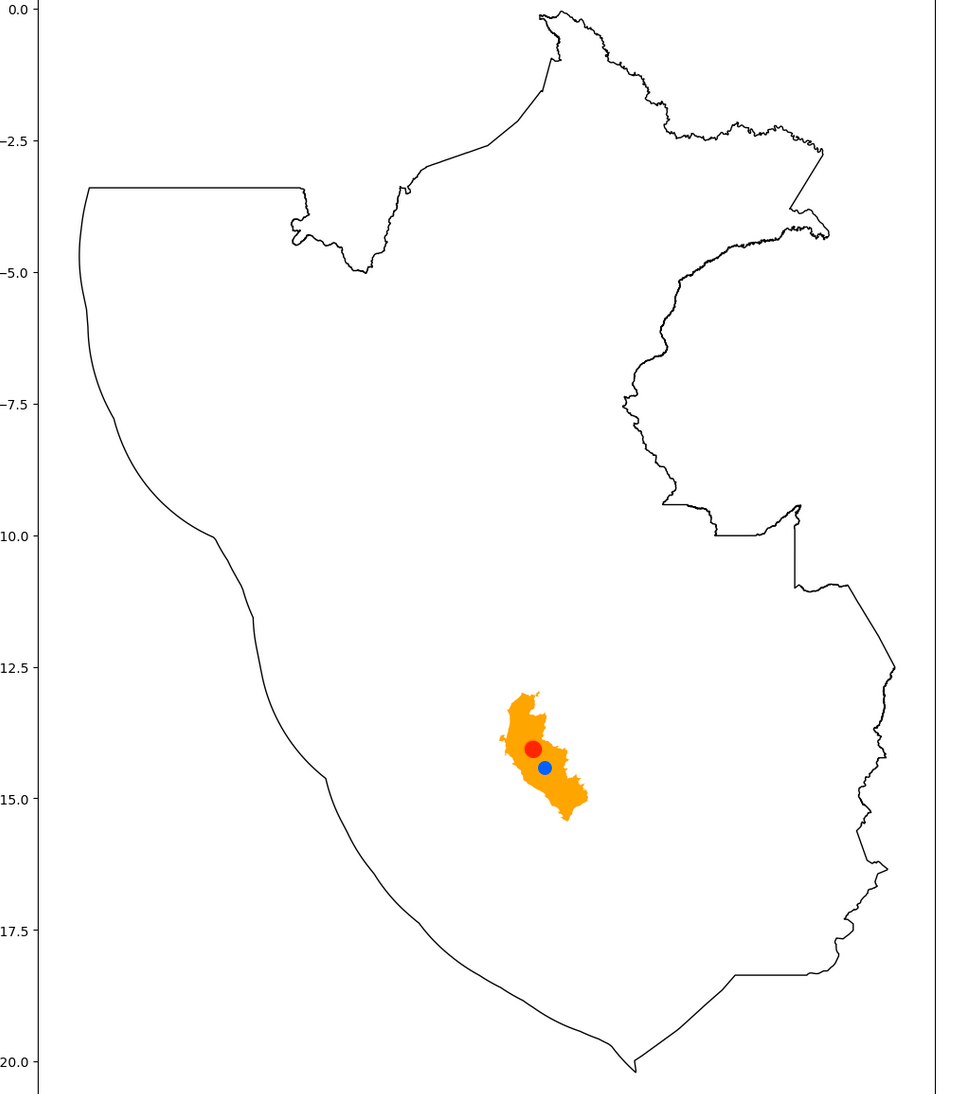
\includegraphics[width=0.4\textwidth]{../images/Ica.png}
    \caption{Géocodage par Open Street Map de la province d'Ica et (centroïde en bleu) et de la ville d'Ica (en rouge).}
    \label{fig:Ica}
\end{wrapfigure}

Les informations géographiques de la base de données étant soit très larges soit très précises, le géocodage n'était pas directement fonctionnel. Les principales difficultés reposaient sur les noms des lieux. Plusieurs toponymes étaient en langues amérindiennes (principalement en aymara ou en quechua), or l'orthographe de ces langues est encore en cours de standardisation. Ainsi, certaines lettres sont interchangeables comme le \og c \fg, le \og k \fg \:et le \og q \fg, ou le \og o \fg \:et le \og u\fg, ou encore le \og i \fg \:et le \og e \fg. Ces variations orthographiques posent problème puisque que Nominatim repose sur l'orthographe des noms pour les trouver dans la base de données d'Open Street Map. Au sein de cette dernière, les variations orthographiques n'apparaissent pas et donc ne sont pas prises en compte au moment du géocodage. Par ailleurs, au Pérou et en Bolivie, il est commun d'avoir le même toponyme pour différents niveaux administratifs, comme nous pouvons le voir sur la figure \ref{fig:Ica}. Une désambiguïsation était donc nécessaire pour ces cas, en spécifiant le niveau administratif du lieu. Enfin, neuf lieux de découvertes textiles étaient des sites archéologiques, pour lesquels une information numérique était accolée au toponyme, référençant la zone précise du site de provenance. Cette information numérique était prise en compte comme une information de numéro de rue par Nominatim qui renvoyait systématiquement une localisation erronée. Ces erreurs ont été modifiées à la main en amont du géocodage et la valeur \og Rapa Nui \fg \:a été associée aux cas irrésolus.


\subsection{Un géocodage robuste ?}
Le processus de géocodage se compose d'allers-retours entre les résultats fournis par l'API d'Open Street Map, les points renseignés sur la carte et les frontières des régions dessinées sur QGIS.

 \begin{figure}[!h]
	\begin{center}
		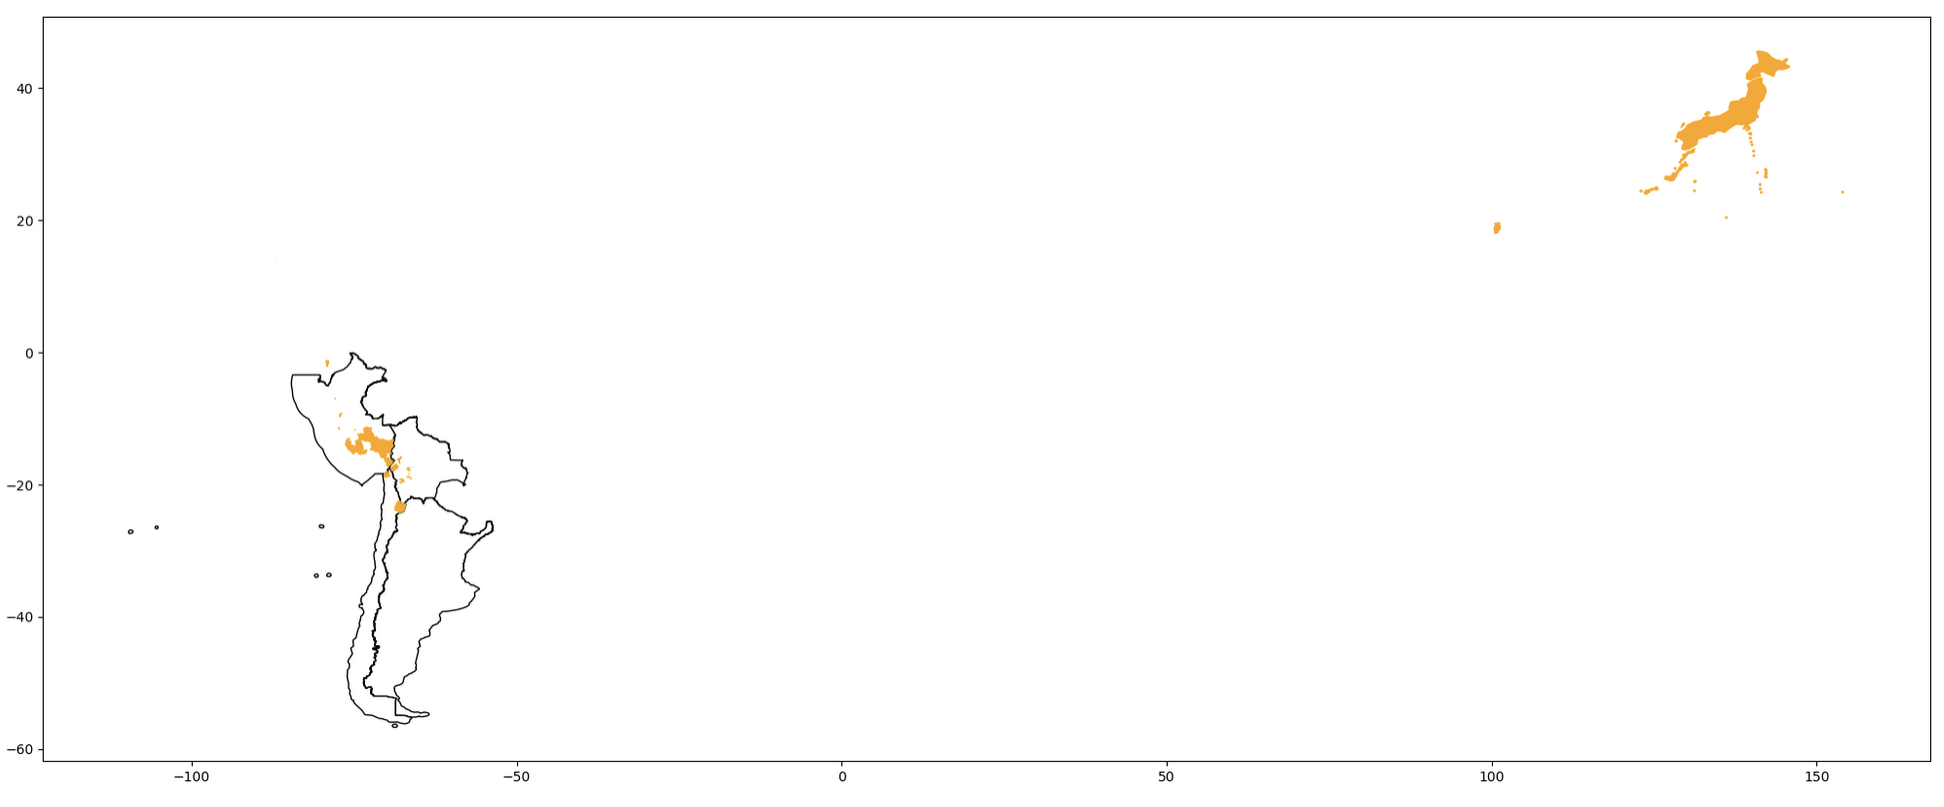
\includegraphics[width=15cm]{../images/erreursGeocodage.png}
		\caption{Première tentative de géocodage.}
		\label{fig:erreurGeocod}
	 \end{center}
\end{figure}

Les premières tentatives étaient infructueuses, comme nous pouvons le voir sur le premier résultat obtenu. L'apparition du Japon sur la carte s'explique par la prise en compte des valeurs nulles -- NaN --  en tant que nom de région japonaise. En remplaçant les valeurs nulles par \og Rapa Nui \fg, nous avons pu réduire le résultat du géocodage à la zone andine. Par ailleurs, en croisant les noms de lieux qui n'étaient pas géoréférencés dans l'API d'Open Street Map avec certaines monographies archéologiques et ethnographiques sur la zone andine, nous avons pu fournir à l'API une approximation du lieu, notamment en fournissant un élément géographique voisin. Par exemple, pour les villages de Jukumani-Laymi et de Laymi, Laurence Charlier Zeineddine qui a fait son terrain dans cette zone nous indique qu'ils ont été regroupés sous le nom de \og Chayanta \fg\footcite[par.~12]{charlierzeineddineChapitreLikIchiri2015}. Il en est de même pour le village de K'ultha que n'arrivait pas à géolocaliser l'API. Denise Y. Arnold et Elvira Espejo indiquent que les villages de Qaqachaka et K'ultha sont voisins\footcite[p.~304]{arnoldWovenTechniquesSocial2014}, ce qui nous a permis. de référencer Qaqachaka et K'ultha avec l'orthographe \og Kaka Chaca \fg \:reconnue par Open Street Map. Toutefois, dans le cas des textiles ethnographiques, se pose la question de l'anonymisation, pratique commune chez les ethnologues pour protéger leurs enquêté\inclusives{e}. Dans le cas de la base de données, il semble que, puisque ce sont les textiles qui sont identifiés, les chercheurs n'ont pas eu recours à une anonymisation géographique, si c'est le cas ils ne l'ont pas spécifiée.
Toutefois, comment être certains que les points géoréférencés sont réellement sur les lieux référencés par les chercheurs ? \\

Face à ces questions, nous avons mis en place un processus automatique de vérification, ou du moins de limitation, des erreurs. Il s'agit de vérifier que les points géocodés sont bien dans les régions associées aux textiles. Tout d'abord, il a fallu mettre de côté les valeurs nulles ou erronées qui ont été indiquées comme \og Rapa Nui \fg \:et pour lesquelles nous savons que le point précis n'est pas dans la région renseignée. Deux cas d'erreurs sont apparus au moment de la vérification : les éléments à la frontières des régions et les éléments ostensiblement mal géocodés. Dans le premier cas, après vérification de la véracité de la localisation des points concernés, nous avons pu redessiner les régions sur QGIS pour qu'elles les incluent. Dans le second cas, c'est à l'étape de géocodage qu'il a fallu modifier le nom fourni, notamment en rajoutant le pays ou le niveau administratif afin de récupérer un point correctement géolocalisé.

Nous obtenons les résultats finaux suivants. La première ligne correspond aux erreurs de géocodage calculées et la seconde à ce même nombre d'erreurs en enlevant les valeurs nulles qui apparaissent comme des erreurs lors de la vérification. Ainsi, nous n'avons aucune erreur pour les lieux de découverte et seulement deux erreurs pour les lieux de production. Ces deux erreurs sont liées à la forme des régions dessinées sur QGIS. La première est sur le Lac Titicaca, en suivant la frontière peruano-bolivienne du lac un des points est situé en Bolivie alors qu'il est renseigné comme péruvien dans la base de données, avec une erreur de moins d'un kilomètre. La seconde erreur n'est pas non plus une erreur de géocodage mais une erreur de frontières régionales. Le point est bien géocodé sur les Salinas de Garcí Mendoza mais il est associé à l'Altiplano Sud dans la base de données alors qu'au vu des autres points, il fait plutôt parti de l'Altiplano Central.

\clearpage
  
 \begin{figure}[!h]
	\begin{center}
		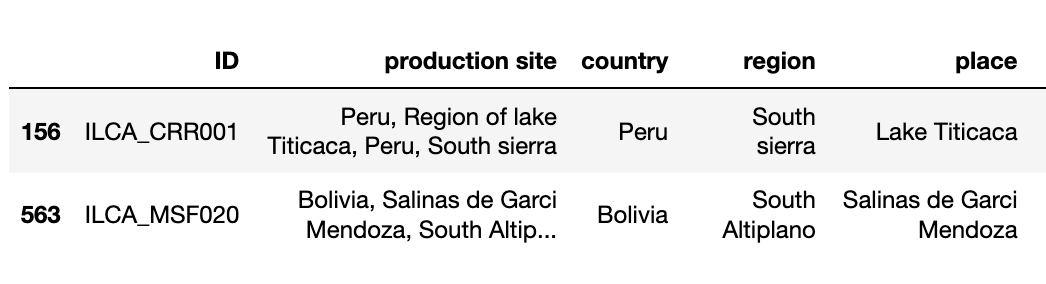
\includegraphics[width=12cm]{../images/verif_prod3bis.png}
		\caption{Erreurs finales pour les lieux de production.}
		\label{fig:erreur_verif}
	 \end{center}
\end{figure}

La vérification du géocodage a eu lieu tout au long du traitement des données. Ainsi, au moment du calcul des distances entre lieu de découverte et lieu de production des textiles, les distances entre les points géocodés correspondent aux lieux présent dans la base de données (voir tableau page \pageref{fig:distancetab}). Une partie de la vérification se fait en restant au plus proche des données initiales pour les confronter aux données géographiques produites lors du géocodage et des analyses suivantes.

\subsection{Cartographier la répartition des textiles de la base de données}

\begin{wrapfigure}{r}{0.4\textwidth}
    \centering
    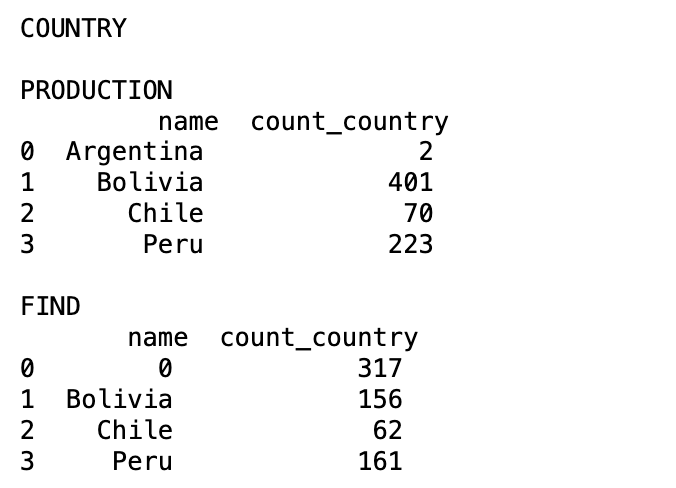
\includegraphics[width=0.4\textwidth]{../images/count_country.png}
    \caption{Nombre de textiles disponibles par pays.}
    \label{fig:tab_count}
\end{wrapfigure}

Pour obtenir la répartition géographique des pièces textiles de la base de données dans la zone andine, nous pouvons commencer par regarder leur répartition avec différents niveaux de granularité.

Dans le cas des pays, les statistiques nous renseignent sur les choix réalisés au sein de la base de données. Le Pérou détient plus de textiles découverts, conséquence de la meilleure conservation des textiles sur la côte. Dans le cas des lieux de production, la concentration bolivienne s'explique par la répartition des musées dont les collections composent la base de données. En effet, les collections ethnographiques de la base de données sont principalement issues de musées boliviens. Cette répartition est donc à la fois une conséquence de la constitution de la base de données et une conséquence de la réalité textile. Toutefois, observer la répartition par pays nous fournit peu d'informations sur les textiles dans la zone andine. C'est pourquoi affiner la granularité au niveau régional nous permettra de mieux saisir cette répartition.

\clearpage

\begin{figure}[!h]
    \begin{minipage}[c]{.5\linewidth}
            \begin{center}
                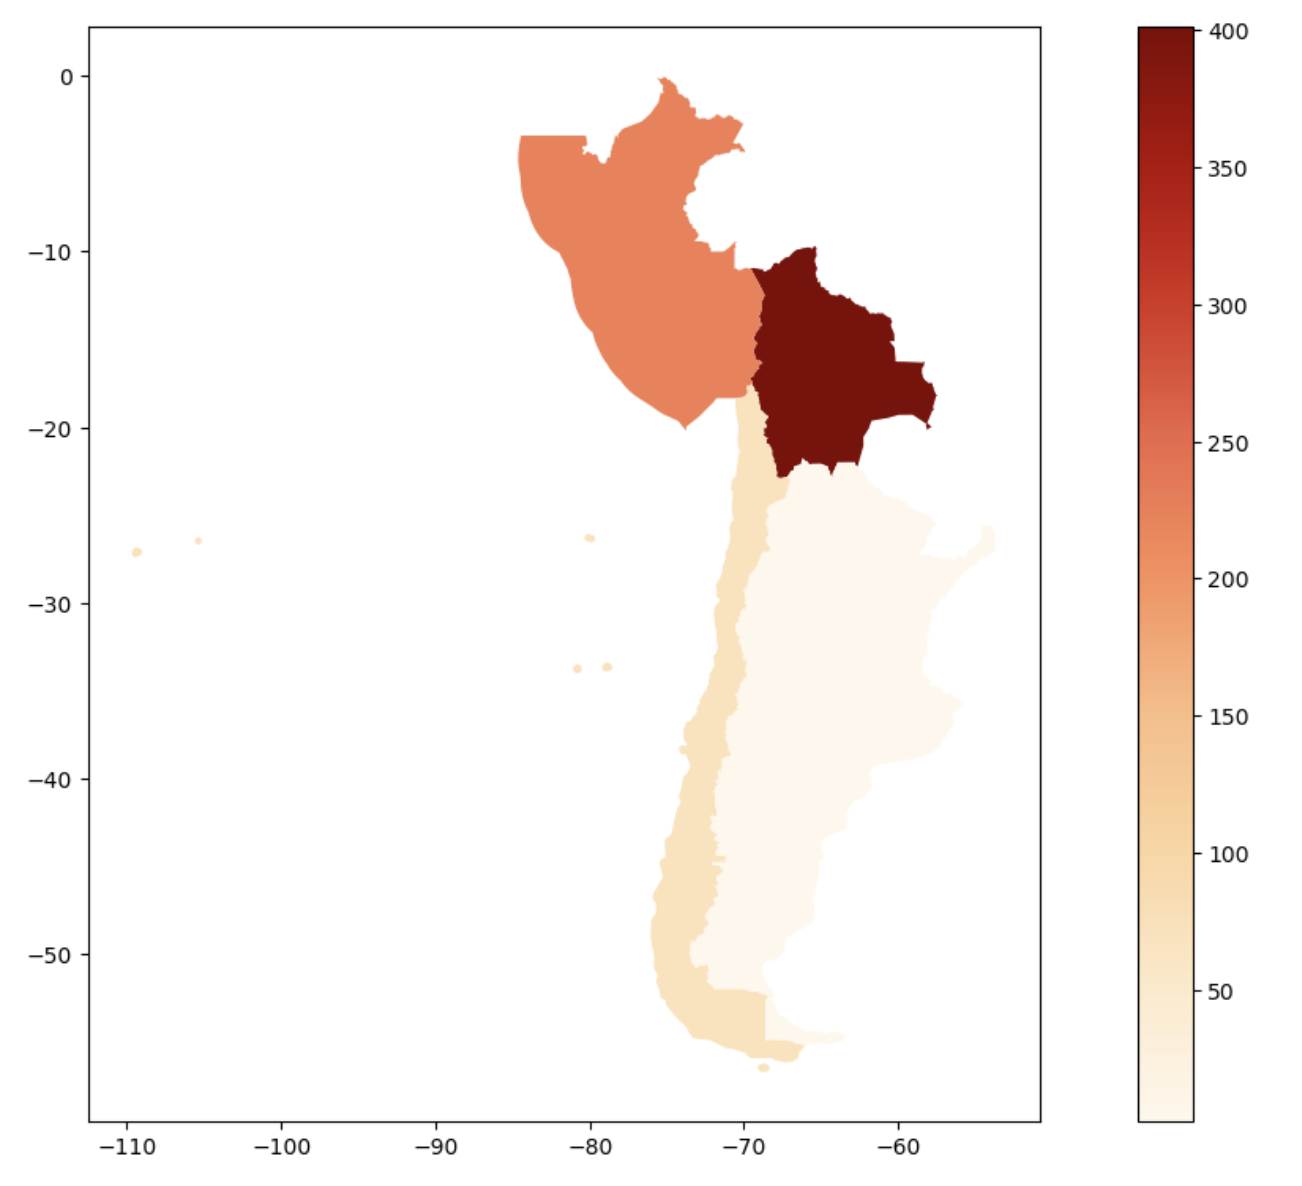
\includegraphics[height=8cm]{../images/map_count_prod.png}
            \end{center}
    \end{minipage}
        \begin{minipage}[c]{.5\linewidth}
        \begin{center}
        		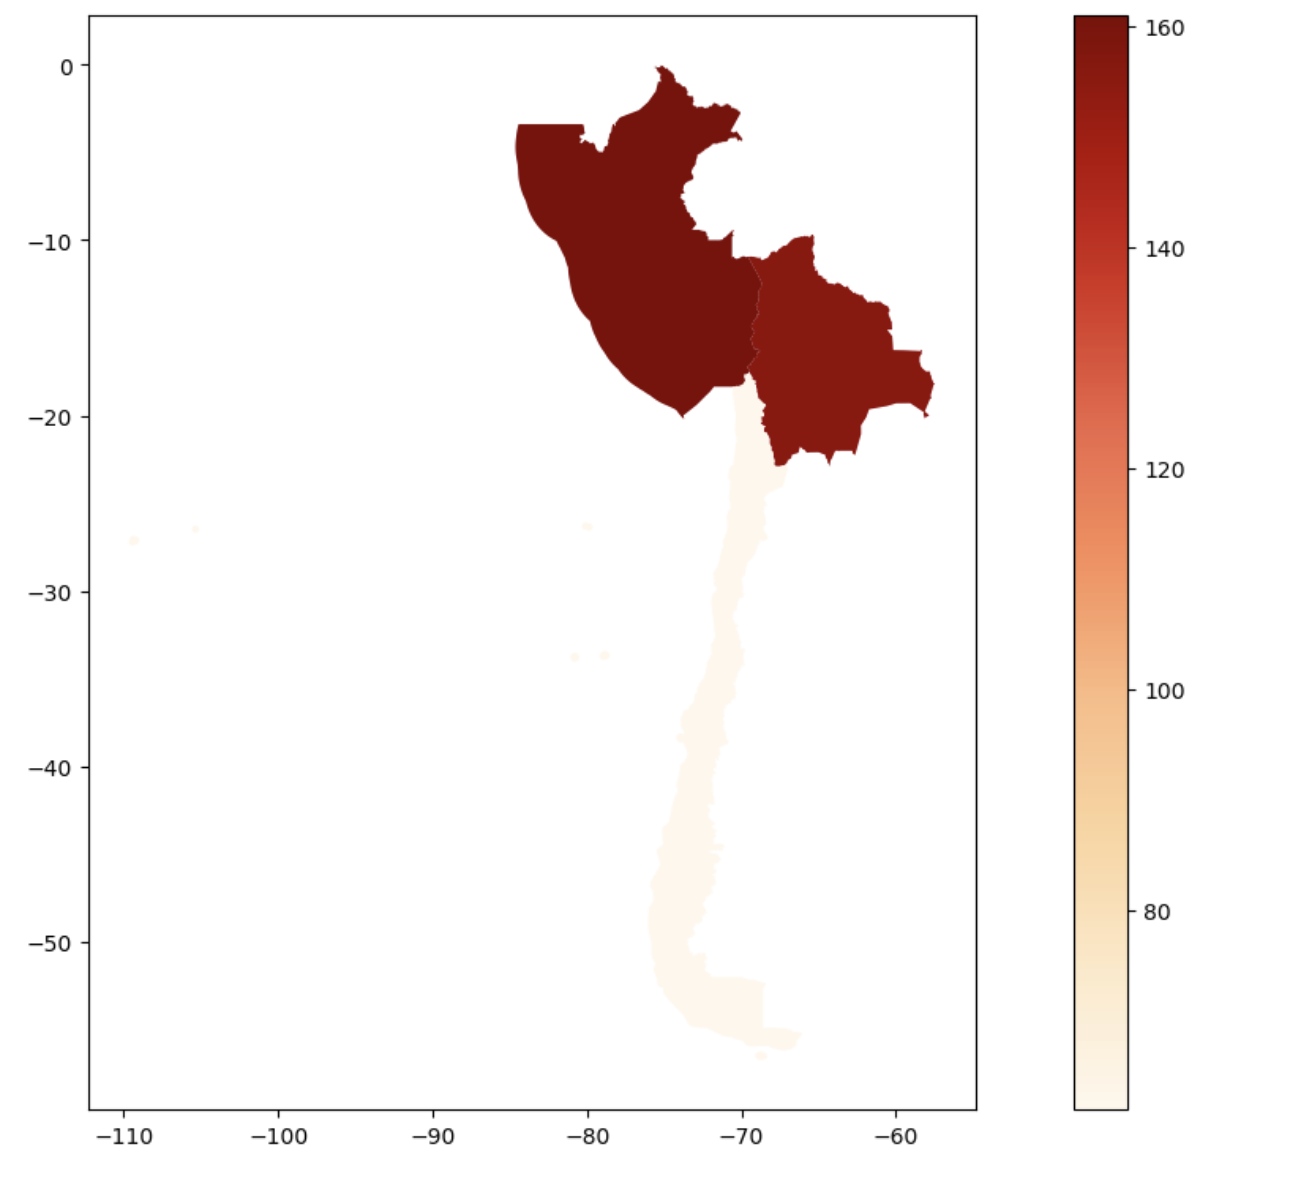
\includegraphics[height=8cm]{../images/map_count_find.png}
	\end{center}
    \end{minipage}
    \caption{Nombre de textiles par pays pour les lieux de productions et pour les lieux de découvertes.}
    \label{fig:geo_count_country}   
\end{figure}

La répartition au niveau régional nous donne des indications similaires mais de manière plus fine. La concentration des textiles produits dans l'Altiplano nord (229 pièces sur 696) nous fournit une information sur la construction de la base de données. L'ILCA a fourni au projet un ensemble de 158 maquettes textiles contemporaines, reproduites dans l'Altiplano nord à partir de motifs locaux imités (voir page \pageref{fig:maquette}). En retirant ces 158 maquettes, nous obtenons une répartition des textiles produits relativement équilibrée dans les hautes-terres.

Les régions de découvertes des textiles sont concentrées dans deux régions, la côte centrale péruvienne et l'Altiplano central. Dans le cas de la côte centrale, il s'agit uniquement de textiles archéologiques, principalement de l'Intermédiaire Récent. Dans le cas de l'Altiplano central, 70\% des textiles \og découverts \fg \:dans la zone sont des textiles ethnographiques.

\begin{figure}[!h]
    \begin{minipage}[c]{.5\linewidth}
            \begin{center}
                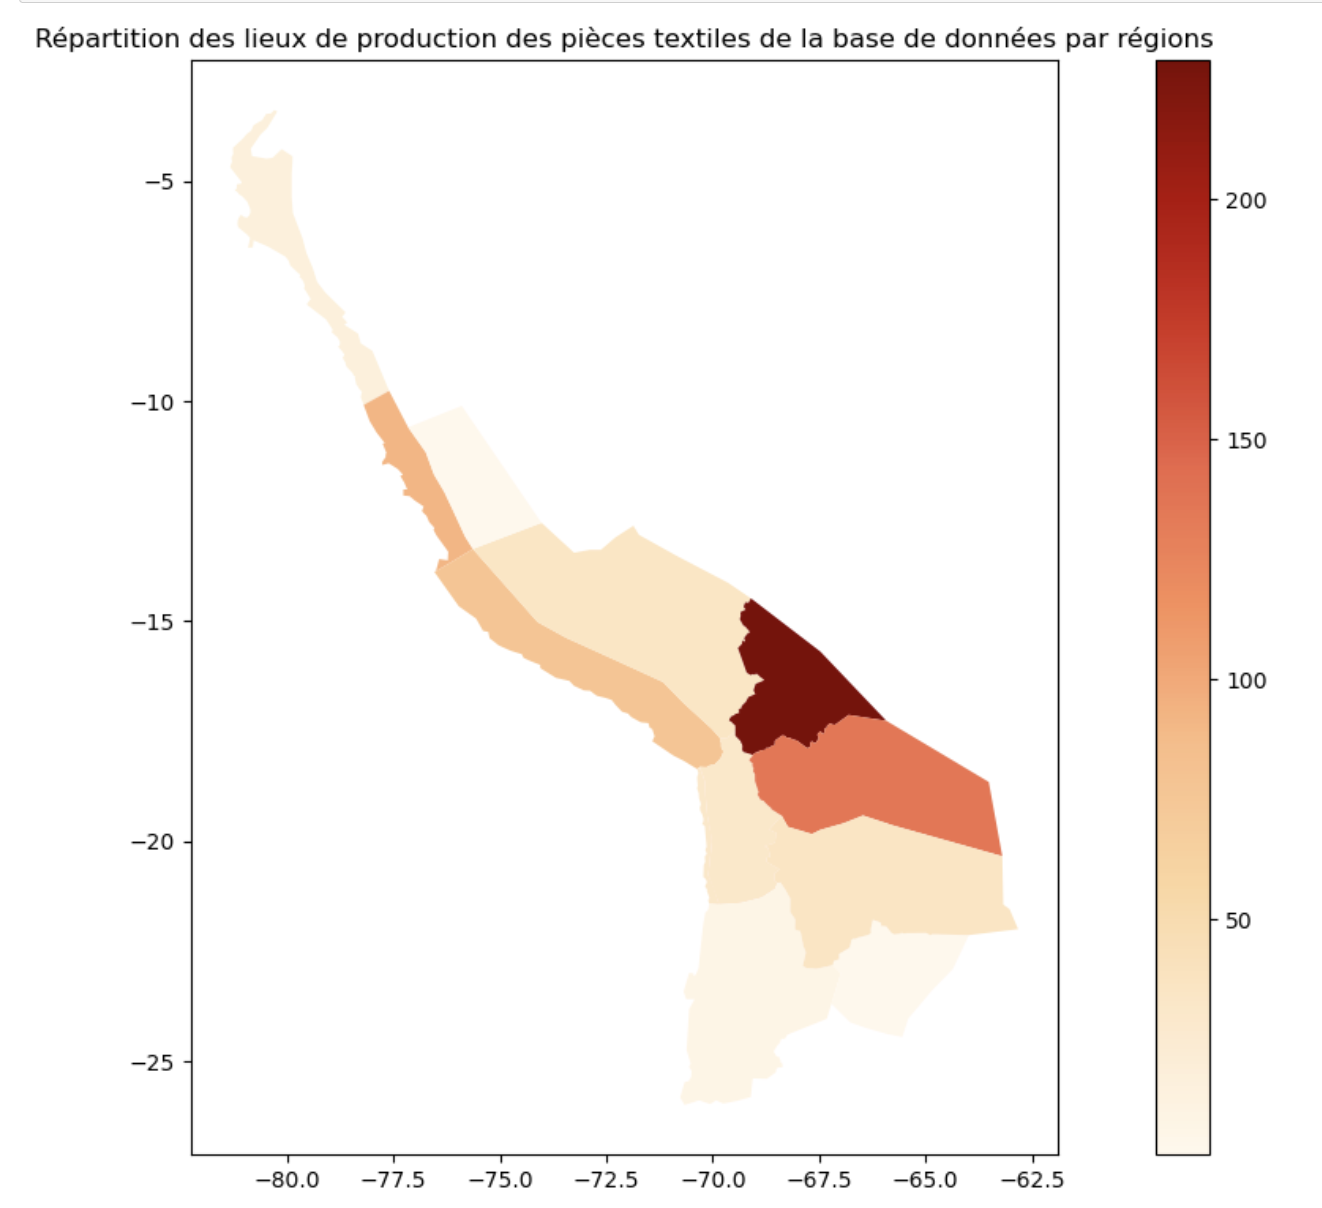
\includegraphics[height=7cm]{../images/geo_region_prod.png}
            \end{center}
    \end{minipage}
        \begin{minipage}[c]{.5\linewidth}
        \begin{center}
        		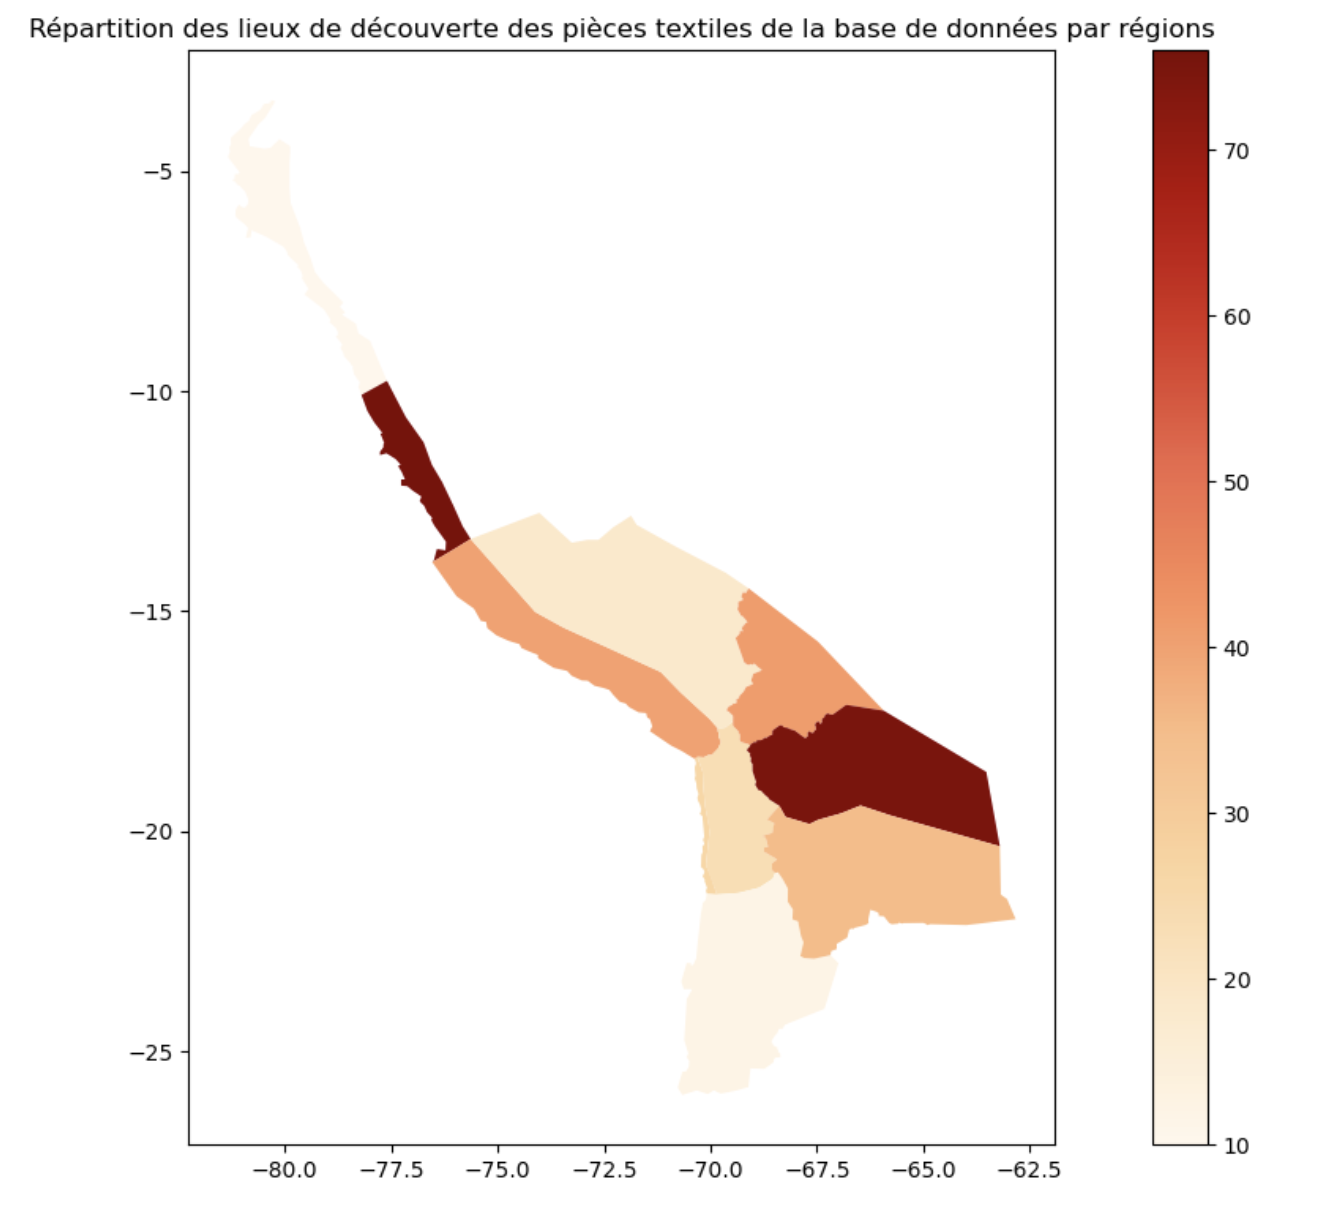
\includegraphics[height=7cm]{../images/geo_region_find.png}
	\end{center}
    \end{minipage}
    \caption{Répartition par région textiles du nombre de textiles pour les lieux de productions et pour les lieux de découvertes.}
    \label{fig:geo_count_region}   
\end{figure}

\clearpage

\begin{figure}[!h]
    \begin{minipage}[c]{.5\linewidth}
            \begin{center}
                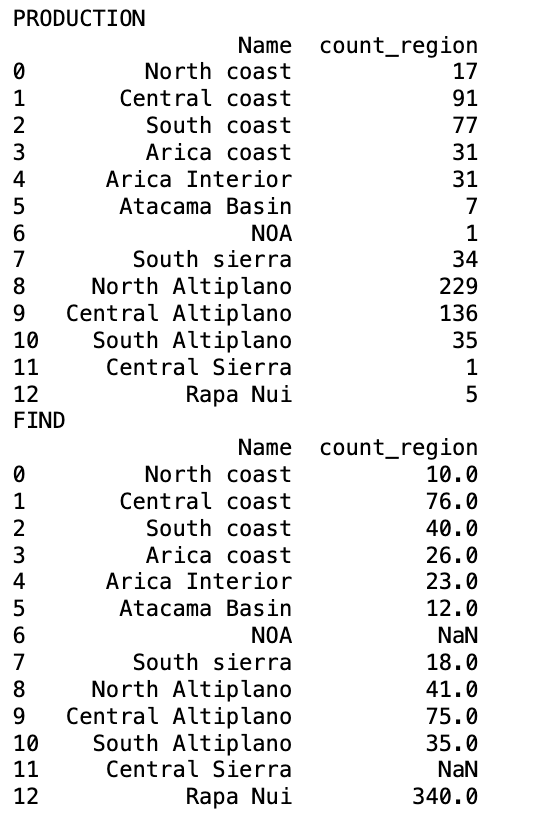
\includegraphics[height=8cm]{../images/count_region.png}
            \end{center}
            \caption{Nombre de textiles disponibles par régions.}
            \label{fig:tab_region_count}   
    \end{minipage}
\hspace{5pt}
        \begin{minipage}[c]{.5\linewidth}
        \begin{center}
        		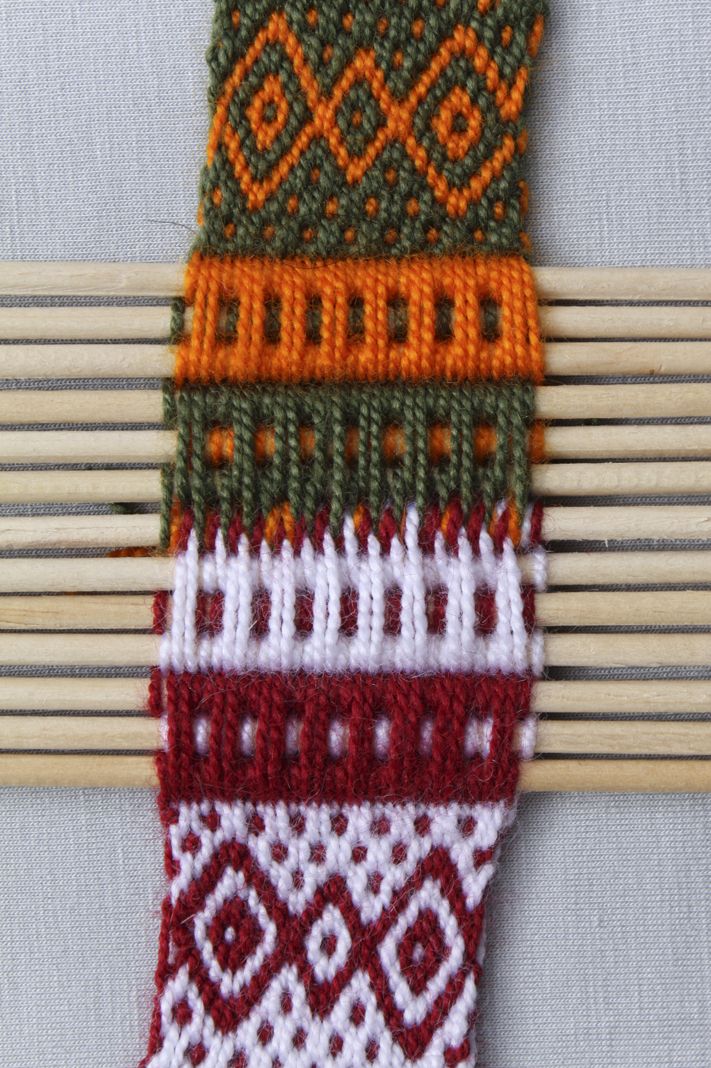
\includegraphics[height=8cm]{../images/MEE008A_IMG_7128.jpg}
	\end{center}
	\caption{Maquette réalisée par des tisserandes de l'Altiplano nord et données à l'ILCA. \\ Référence dans la base de données : MEE008A}
	\label{fig:maquette}   
    \end{minipage}
\end{figure}

Dans une logique exploratoire et de présentation des données, nous pouvons réaliser des cartes interactives en utilisant les localisations précises des textiles récupérées par le géocodage. Pour cela, nous avons utilisé la librairie Folium qui permet de réaliser des cartes avec Leaflet, un outil de cartographie en langage JavaScript. L'option \og cluster \fg \: dans la carte permet une meilleure visibilité en regroupant les points les plus proches. En zoomant, il est possible de voir la localisation précise et en cliquant sur le point, l'utilisateur peut obtenir l'image du textile, son identifiant dans la base de données, ainsi que son lieu de production ou de découverte selon la carte.
Pour pouvoir afficher les images, nous avons eu recours à un script de redimensionnement qui réduit le plus petit côté de l'image à 100 pixels et le plus grand proportionnellement à cette réduction\footnote{Les cartes interactives sont accessibles aux liens suivants: \url{https://lisebernard.github.io/carte_find_clustering.html} et \url{https://lisebernard.github.io/carte_prod_clustering.html}. Le script de redimensionnement des images est nommé rescale\_images.ipynb.}.

\begin{figure}[!h]
	\begin{center}
		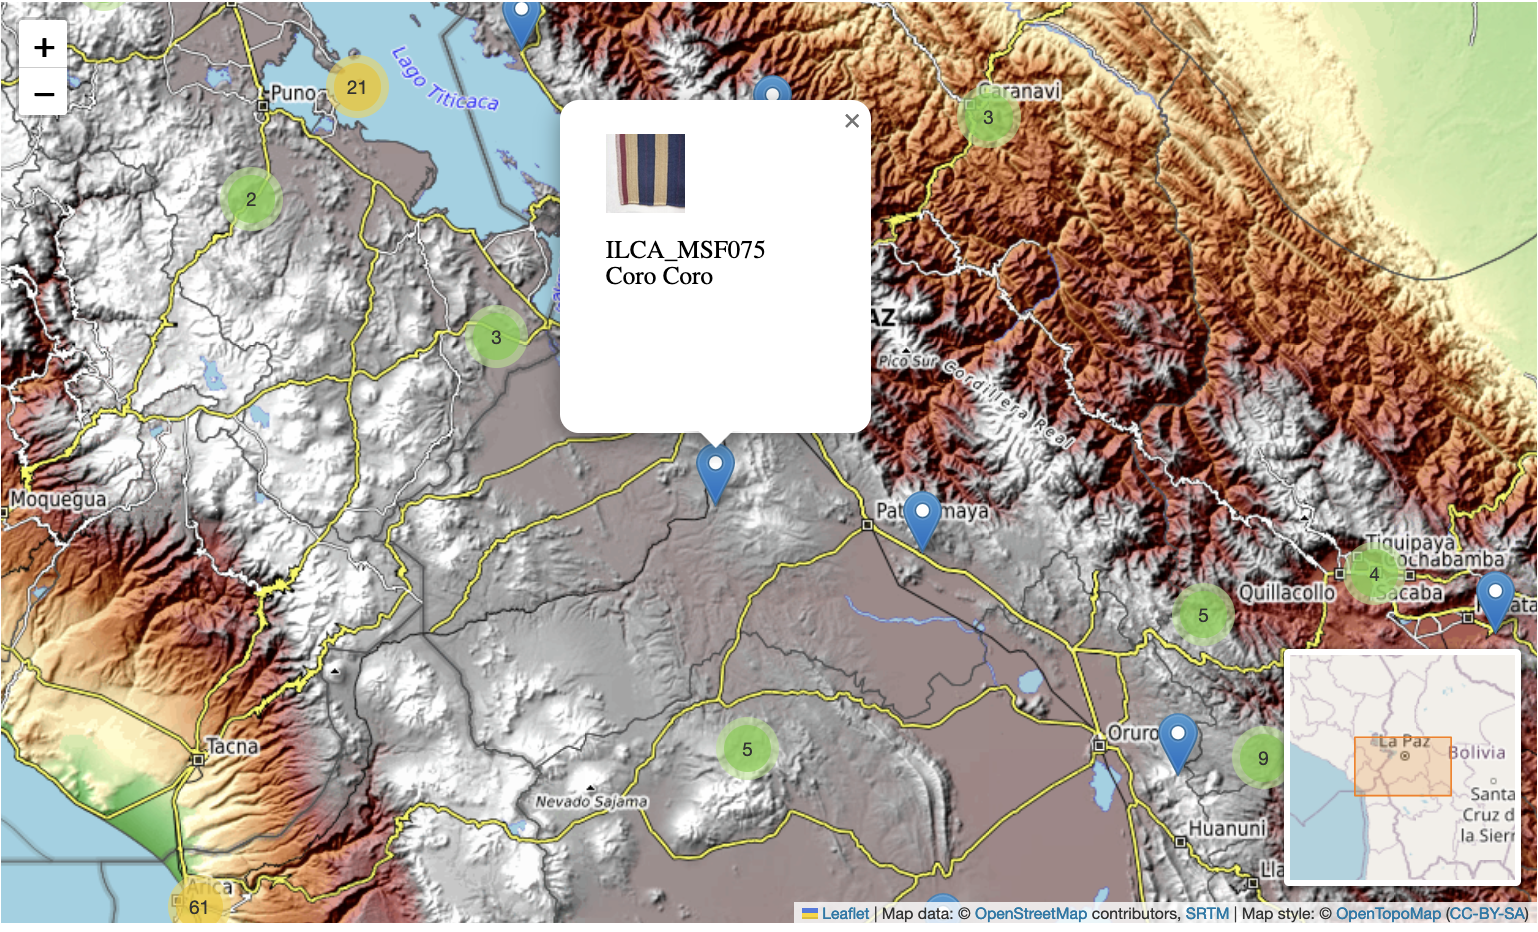
\includegraphics[width=12cm]{../images/carte_leaflet2.png}
		\caption{Détail de la carte interactive avec affichage d'une photographie du textile ainsi que de son identifiant et son lieu de production.}
		\label{fig:leaflet}
	 \end{center}
\end{figure}

\clearpage


\section{Répartition et mobilités des textiles de la base de données}

\subsection{Mettre en évidence les foyers textiles grâce aux cartes de densité}

Pour essayer de détecter les foyers les plus denses en productions et en découvertes textiles, nous pouvons avoir recours à des cartes de densité\footnote{Les cartes de densité ont été réalisées en Python avec la librairie Matplotlib. Leur code est disponible dans le script traitement\_maps.ipynb.}. Ces cartes permettent de visualiser les zones comportant le plus d'entités ponctuelles (de points) sur la carte. Elles illustrent la répartition des données. Pour cela, nous appliquons aux points une estimation par noyau (ou \textit{kernel density estimation}) qui estime la densité de probabilité d'une variable aléatoire non-paramétrique. Dans notre cas, il faut retirer la variable \og Rapa Nui \fg \:dont la prégnance déséquilibre le calcul. Pour avoir le détail de la densité des points, nous pouvons également réaliser des cartes interactives avec Leaflet qui prennent en compte le nombre de textiles associés à un point. Contrairement aux cartes précédentes, elle permettent de récupérer à la fois la répartition globale et l'information ponctuelle de densité\footnote{Les cartes interactives sont accessibles aux liens suivants : \url{https://lisebernard.github.io/heatmap_prod.html} et \url{https://lisebernard.github.io/heatmap_find.html}}. Les cartes interactives sont certes un outil exploratoire mais elles viennent également compléter les cartes fixes puisqu'elles permettent d'obtenir le lieux précis et le nombre de textile pour chaque point.

\begin{figure}[!h]
    \begin{minipage}[c]{.5\linewidth}
            \begin{center}
                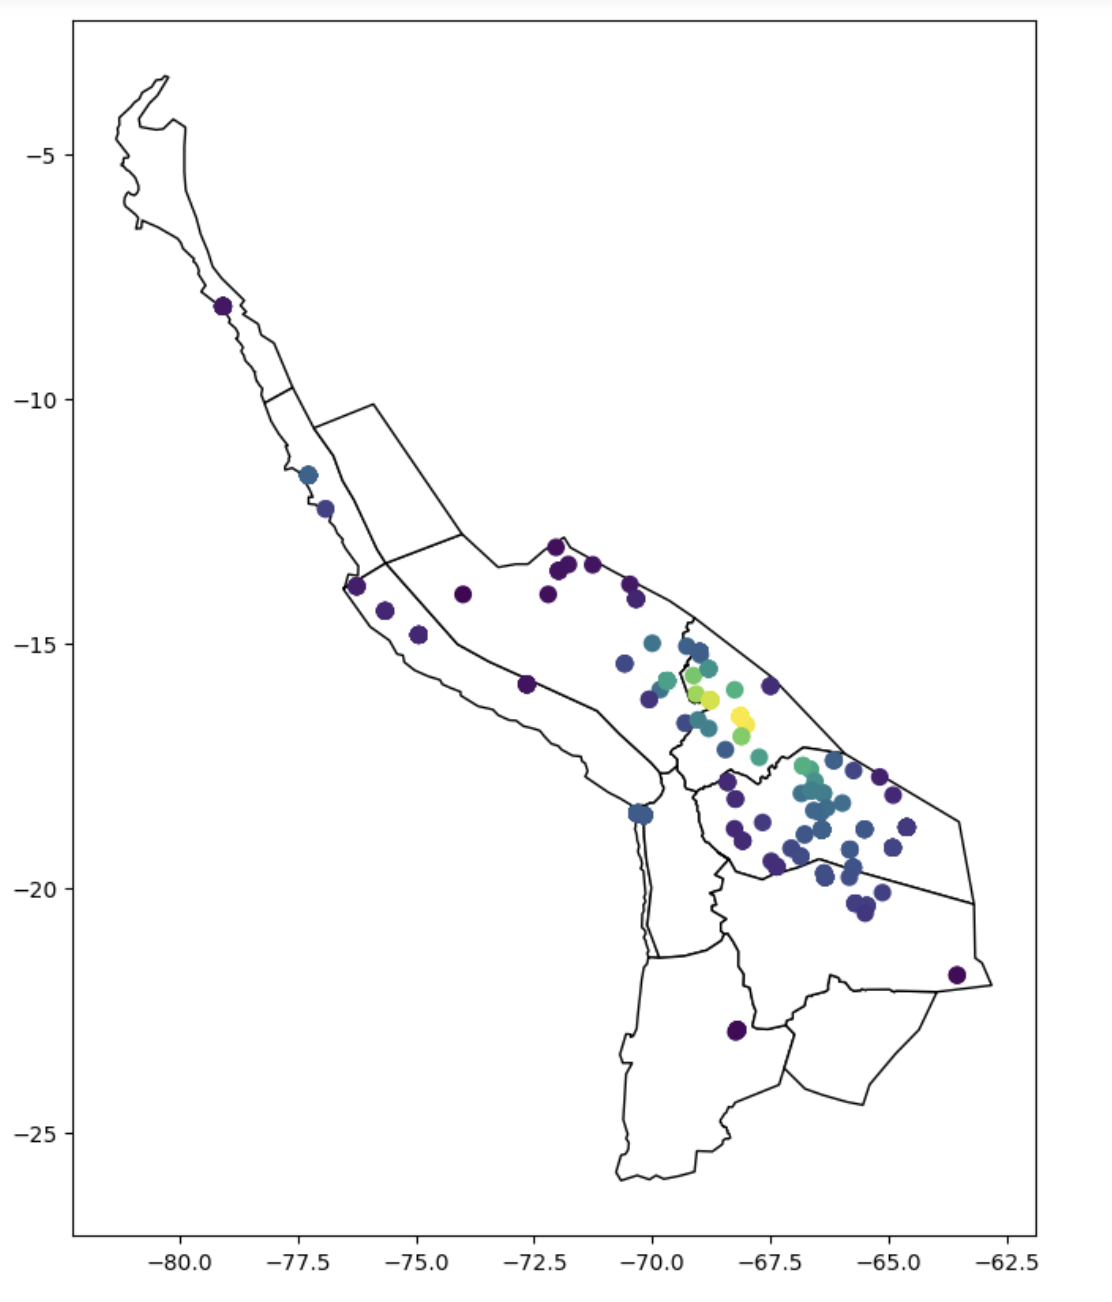
\includegraphics[height=8cm]{../images/densitymapprod.png}
            \end{center}
            \caption{Carte de densité des lieux de production des textiles.}
            \label{fig:densityProd}   
    \end{minipage}
\hspace{5pt}
        \begin{minipage}[c]{.5\linewidth}
        \begin{center}
        		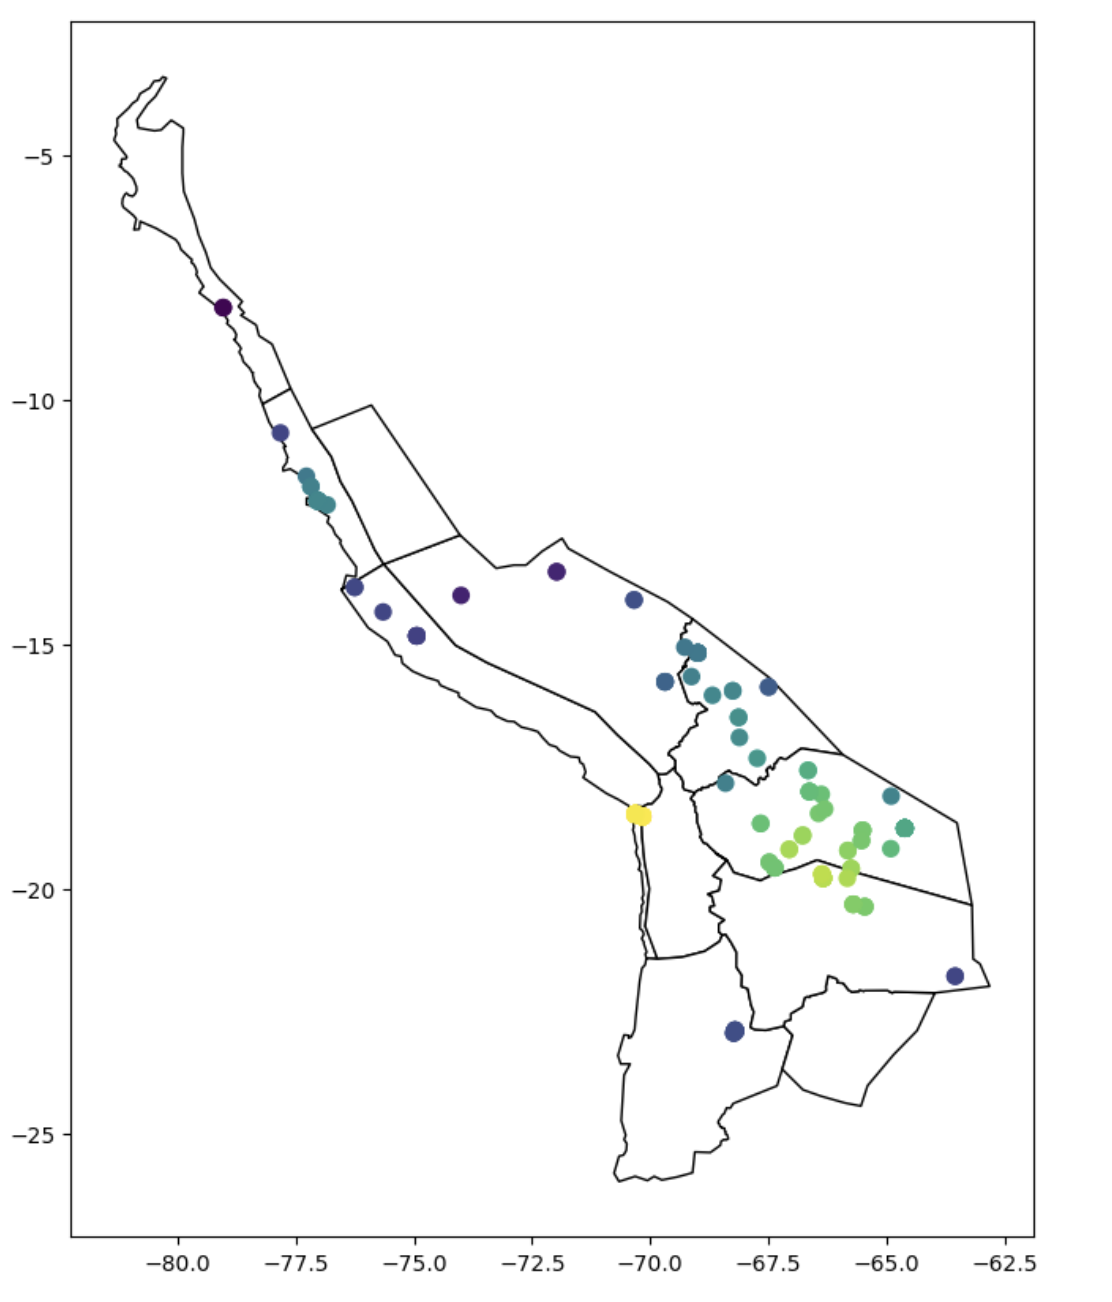
\includegraphics[height=8cm]{../images/densitymapfind.png}
	\end{center}
	\caption{Carte de densité des lieux de découverte des textiles.}
	\label{fig:densityFind}   
    \end{minipage}
\end{figure}

 \begin{figure}[!h]
	\begin{center}
		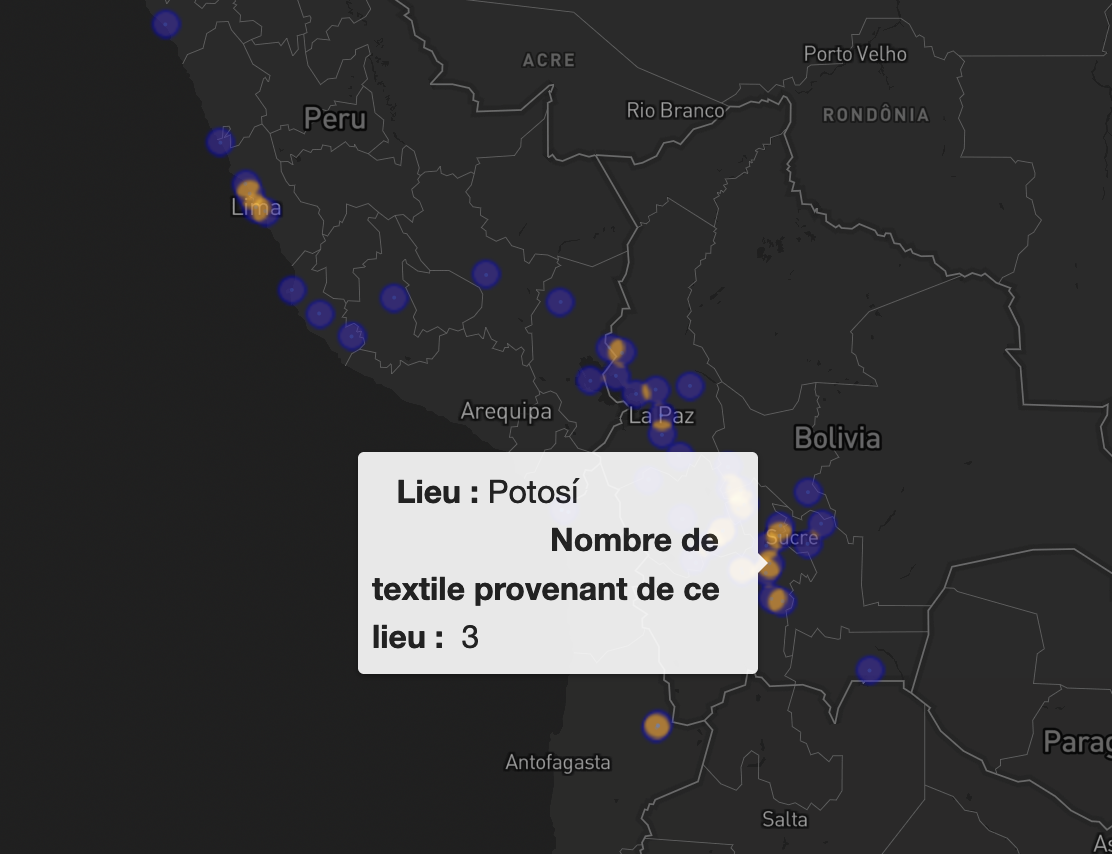
\includegraphics[width=12cm]{../images/heatmap_leaflet.png}
		\caption{Détail de la carte de densité des lieux de production interactive avec affichage du lieu et du nombre de textiles provenant du lieu.}
		\label{fig:leaflet_density}
	 \end{center}
\end{figure}

Dans le cas des lieux de production, un des foyers centraux se trouve dans la région de La Paz (capitale bolivienne). Dans les Andes, les points sont concentrés sur la cordillère Est de l'Altiplano et au niveau du lac Titicaca. Les quelques points épars au nord des hautes-terres sont situés dans la région de Cuzco. Sur la côte, les points sont éparpillés avec un foyer un peu plus important sur la côte centrale au niveau de Lima. 

Dans le cas des lieux de découverte, les foyers en altitude sont plus au sud que pour les lieux de production. Ils se situent plutôt dans la région de Potosí. Sur la côte, la zone d'Arica au sud se distingue largement avec deux foyers archéologiques importants. Au niveau de la côte centrale, la zone de Lima est également dense avec plusieurs foyers archéologiques. Au sud de Lima, on trouve les deux foyers textiles les plus connus et étudiés : Nazca et Paracas.

Pour mieux comprendre la répartition de ces foyers, nous pouvons développer une approche diachronique en produisant des cartes de densité par période étudiée\footnote{Le calcul de densité est calculé indépendamment pour chaque période, les couleurs sur chaque carte ne sont donc pas équivalentes en quantité de textile mais indiquent plutôt une valeur relative de densité d'un lieu par rapport à un autre sur la période étudiée.}. 

Les époques de la période Initiale et de l'Horizon Ancien n'ont qu'un seul point géolocalisé ce qui ne permet pas de réaliser un calcul de densité. Nous pouvons tout de même observer l'origine de ces textiles, l'un sur la côte sud, l'autre au niveau de Lima, sur la côte centrale.

\begin{figure}[!h]
	\begin{center}
		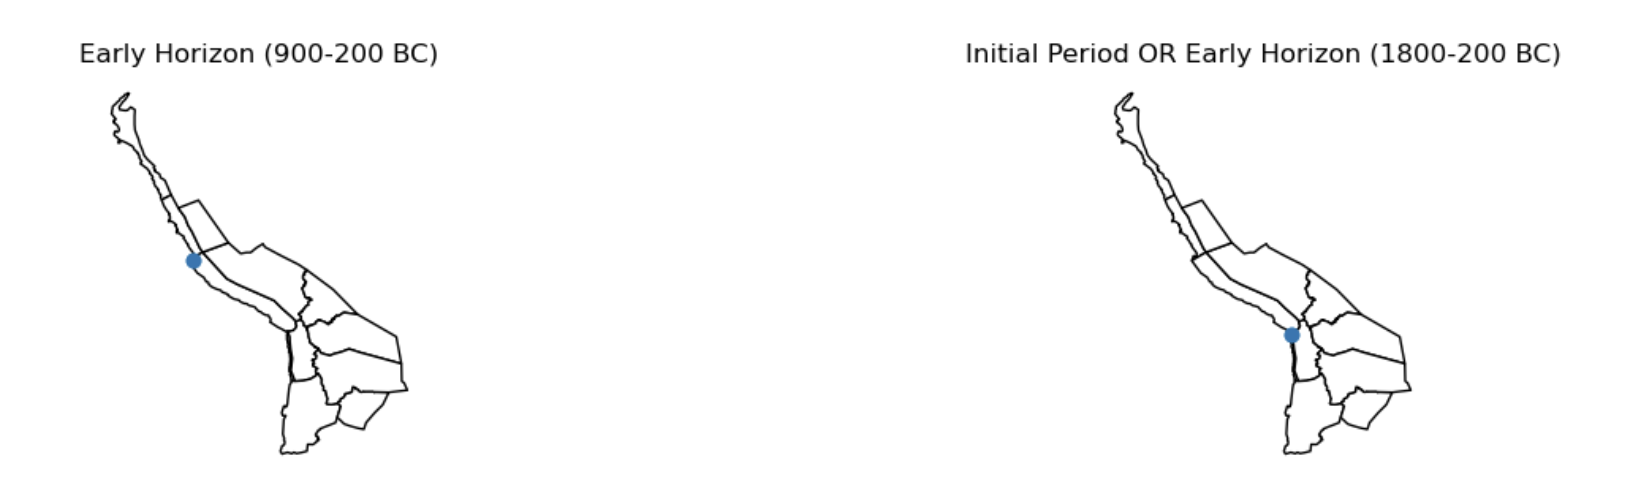
\includegraphics[width=15cm]{../images/carteEH.png}
		\caption{Position des points pour la période Initiale et l'Horizon Ancien.}
		\label{fig:carteEH}
	 \end{center}
\end{figure}

\begin{figure}[!h]
	\begin{center}
		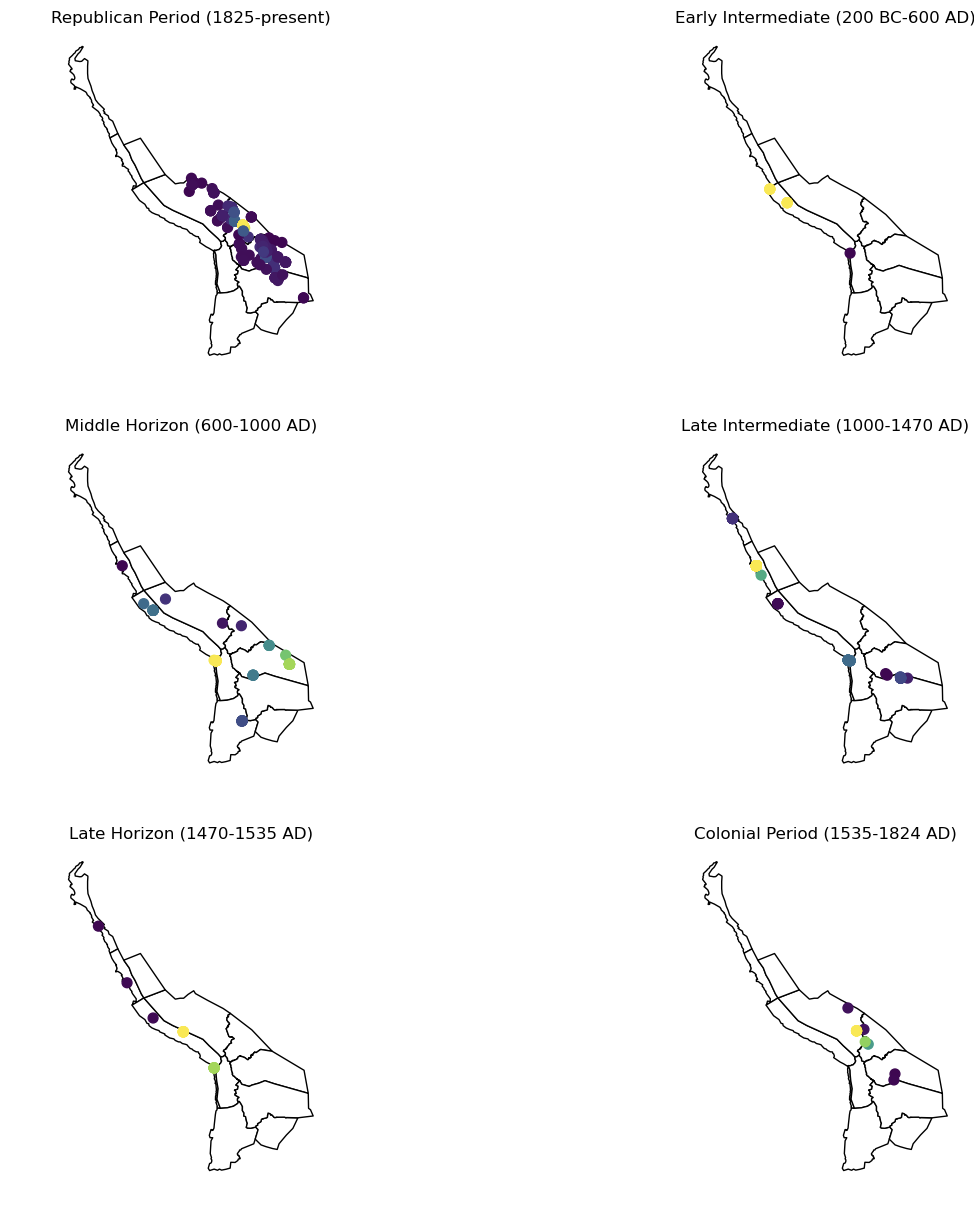
\includegraphics[width=13cm]{../images/diachDensityProd.png}
		\caption{Carte de densité diachronique des lieux de productions des textiles.}
		\label{fig:density_prod}
	 \end{center}
\end{figure}

\noindent Les textiles de la période Intermédiaire Ancienne sont également produits sur la côte, avec deux foyers importants à cette période : Nazca et Paracas\footcite[p.~58-59]{boissiereAtlasAmeriquePrecolombienne2022}.
À partir de l'Horizon Moyen, période marquée par la diffusion des civilisations Huari et Tiwanaku\footnote{Ibid., p.~68-69}, des fragments de textiles sont disponibles sur tout le territoire andin. Les foyers Nazca et Paracas persistent avec un phénomène de métissage entre les styles côtiers et l'influence de l'empire Huari provenant des Andes centrales. L'exemple présenté ici (photographie \ref{fig:VAM012}) montre la persistance du motif de serpents entremêlés relevé dès l'Horizon Ancien\footcite[p.~1]{desrosiersRevisitingOcucajeOpened2008}.

\noindent Tout au sud, le foyer textile dans le désert d'Atacama et à Arica illustre les phénomènes d'échanges à cette période. Les textiles de cette zone sont principalement composés en styles locaux (Cabuza, Maytas-Chiribaya, Coyo ou Quitor) mais des textiles se distinguent par l'influence de la culture Tiwanaku (voir photographie \ref{fig:SPA012}). L'influence Tiwanaku s'observe également dans les hautes-terres boliviennes, à Puqui, avec des textiles de style local mais également un textile qui reprend des éléments iconographiques Tiwanaku, notamment les bordures composées de fils colorés (pour un exemple de textile Tiwanaku, découvert dans les hautes-terres voir page \pageref{fig:MNA037}). Pour le reste des hautes-terres, le foyer principal est le foyer Mojocoya, au sein duquel les textiles sont produits et découverts sur place.

À la période Intermédiaire Récente, les foyers principaux se situent encore sur la côte. Tout au nord, un foyer est composé de textiles Chimú, provenant de la capitale de l'empire éponyme, Chan Chan. À la même période, dans les hautes-terres, c'est la culture Qaraqara qui compose un foyer. Il s'agit d'une \og confédération d'ethnies régionales et de seigneuries préhispaniques \fg \:organisées après la chute de l'empire Tiwanaku\footnote{\cite[p.~309]{oriasReviewQaraqaraCharkaMallku2009}. Citation originale : \textquotedblleft \textit{confederación de etnias regionales y señoríos prehispánicos}\textquotedblright}. Ces textiles sont relativement simples, en terme de techniques et de motifs, puisqu'avec la partition régionale typique des périodes intermédiaires, les styles iconographiques se simplifient\footcite[p.~288]{coveyMultiregionalPerspectivesArchaeology2008}.
\begin{figure}[!h]
    \begin{minipage}[c]{.5\linewidth}
    \begin{center}
     	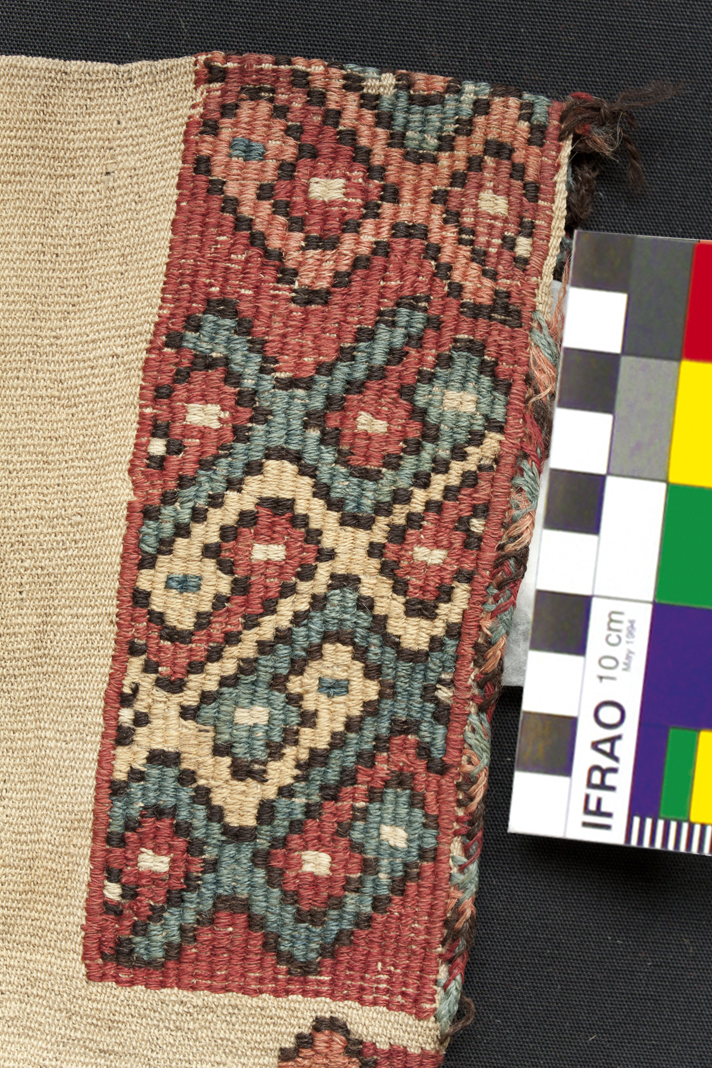
\includegraphics[width=6cm]{../images/VAM012.jpg}
     	\caption{Tunique dans un style qui mélange éléments Nazca et Huari. \\ Référence dans la base de données : VAM012}
    	\label{fig:VAM012}
    \end{center}
    \end{minipage}
    \hspace{5pt}
    \begin{minipage}[c]{.5\linewidth}
        		\begin{center}
         		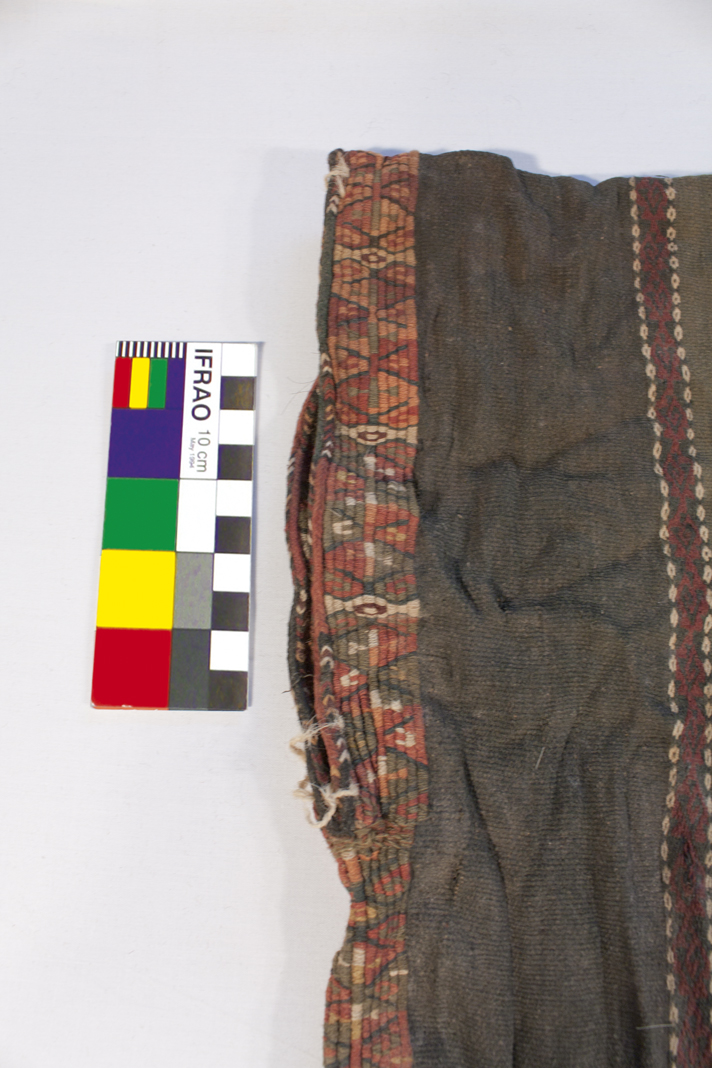
\includegraphics[width=6cm]{../images/SPA012.jpg}
         		\caption{Éléments iconographiques Tiwanaku sur une tunique provenant de la région d'Atacama. \\ Référence dans la base de données : SPA012}
			\label{fig:SPA012}
		\end{center}
	\end{minipage}
\end{figure}

\begin{wrapfigure}{r}{0.4\textwidth}
	\begin{center}
		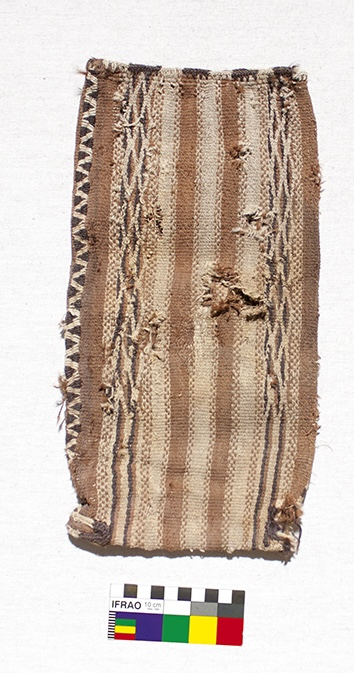
\includegraphics[width=3cm, angle=-90]{../images/MCM014.jpg}
		\caption{Exemple de textile Qaraqara.\\ Référence dans la base de données : MCM014}
		\label{fig:MCM014}
	 \end{center}
\end{wrapfigure}

Au cours de l'Horizon Récent, marqué par le développement de l'empire Inca, les foyers précédents persistent, notamment les Chimú dont la chute arrive en 1470, date du début de l'Horizon Récent dans la base de données. Les textiles de cette période dans la base de données sont tous catégorisés comme Incas. 

Les textiles coloniaux et républicains proviennent exclusivement des hautes-terres du sud du Pérou et de l'Altiplano bolivien. À partir de ces périodes, il est plus compliqué de penser les textiles en termes de foyers de production. Comme déjà mentionné, les espagnols participent amplement à la diffusion des styles entres populations. Les foyers apparaissant sur les cartes sont alors plutôt des indicateurs des collections muséales composant la base de données. Toutefois, elles illustrent bien la disparition progressive des pratiques de tissage sur la côte avec la progression des hautes-terres dans la domination de la pratique textile andine. \clearpage

%Huari : BML106 / MSF041 / MNA014 / MSF051 / MSF060 --> dans la sierra MSF018
%Tiwanaku : BML012 / BML013 / BML013 / MCM025 (pour la côte sud) --> pour Atacama et Arica : SPA003 (provincial) / MMA082-87/MMA087/MMA089-91/MMA093-97/MSF016/MSF029/SPA003/SPA012
%BML087 Chancay pendant Middle Horizon ? 
%Autre cas Tiwanaku dans les hautes-terres : MNA035 / MNA037 /SPA001 / SPA009

\begin{figure}[!h]
	\begin{center}
		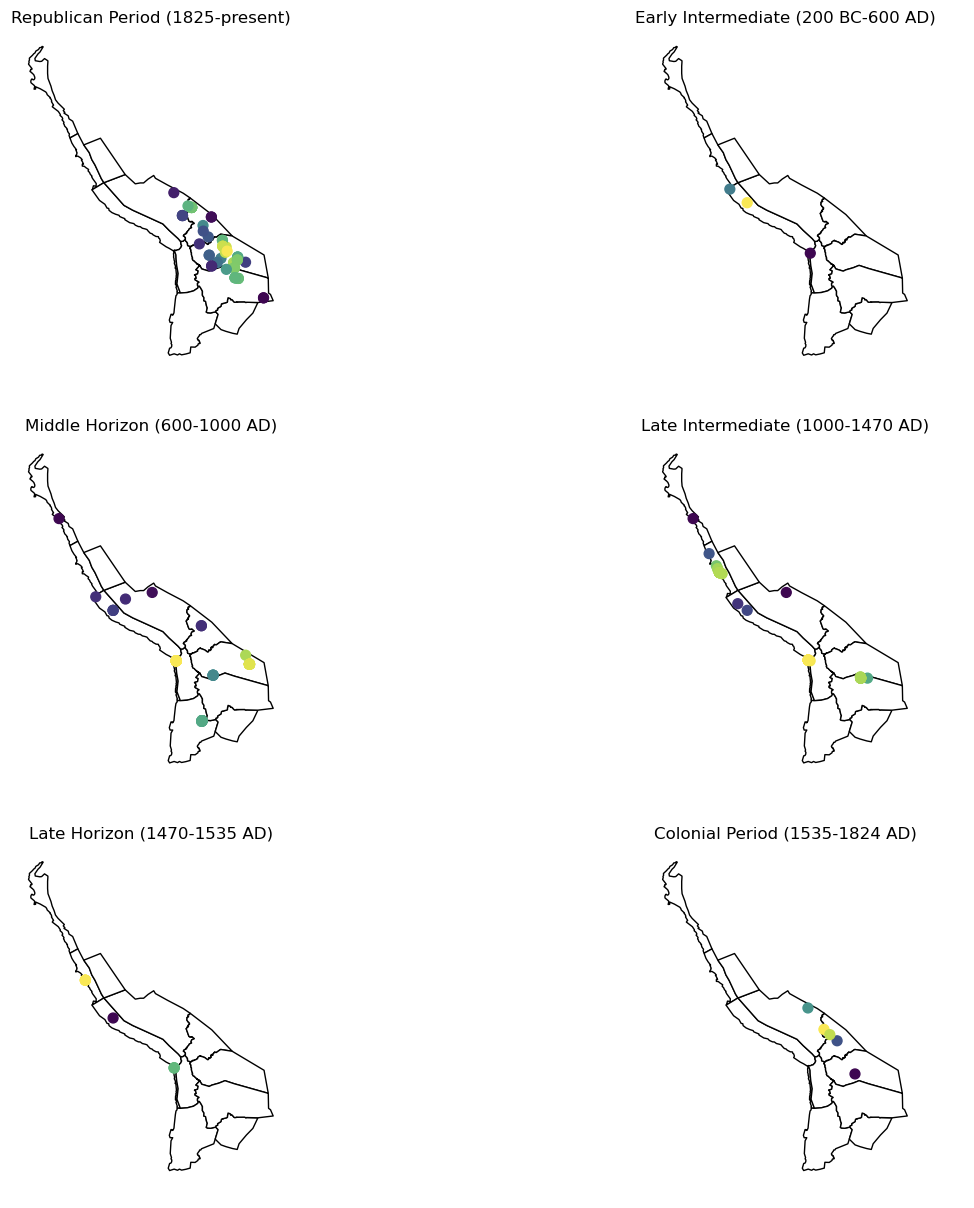
\includegraphics[width=15cm]{../images/diachDensityFind.png}
		\caption{Carte de densité diachronique des lieux de découvertes des textiles.}
		\label{fig:density_find}
	 \end{center}
\end{figure}

Pour les lieux de découverte, les foyers apparaissant sur les cartes de densité sont similaires puisqu'il s'agit principalement des mêmes textiles dont les lieux de production et de découverte se situent au même endroit. Disposant de moins de données pour les lieux de découverte, la répartition de la densité est moins dispersée ce qui donne une densité plus lissée avec moins d'extrêmes. En comparaison avec les lieux de production, à la période Intermédiaire Ancienne, les textiles Paracas sont moins denses que les textiles Nazca. Il en est de même à l'Horizon Moyen, au cours duquel on retrouve les mêmes foyers principaux mais moins de foyers secondaires. Á la période Intermédiaire Récente, les textiles sont concentrés sur la côte avec moins de foyers Qaraqara dans les hautes-terres et plus de concentration à Arica, notamment avec les excavations de la Playa Miller de style Pocoma. Au niveau des côtes centrale et sud, les civilisations côtières dominent avec notamment des textiles Chimú, Ichma et Chancay. À l'Horizon Récent, seuls trois foyers apparaissent le long de la côte avec la persistance d'Arica au sud, Nazca au milieu et Lima au nord. Aux périodes coloniale et républicaine, les foyers de découverte sont moins épars et plus concentrés sur l'Altiplano central. 

\subsection{Saisir les mobilités par des calculs de distances}

Cartographier les textiles nous a permis de saisir leur répartition et leur densité sur le territoire andin. En outre, dans le cas où les textiles disposent d'un lieu de production et d'un lieu de découverte distincts, nous pouvons saisir les circulations physiques des textiles. Ne détenant que deux localisations, un point de départ et un point d'arrivée, nous ne sommes pas en mesure de saisir les parcours des textiles mais nous pouvons saisir certaines circulations avec des distances à vol d'oiseau\footnote{Les calcul de distance et leur cartographique sont disponibles dans le script traitement\_maps.ipynb.}.

\begin{figure}[!h]
	\begin{center}
		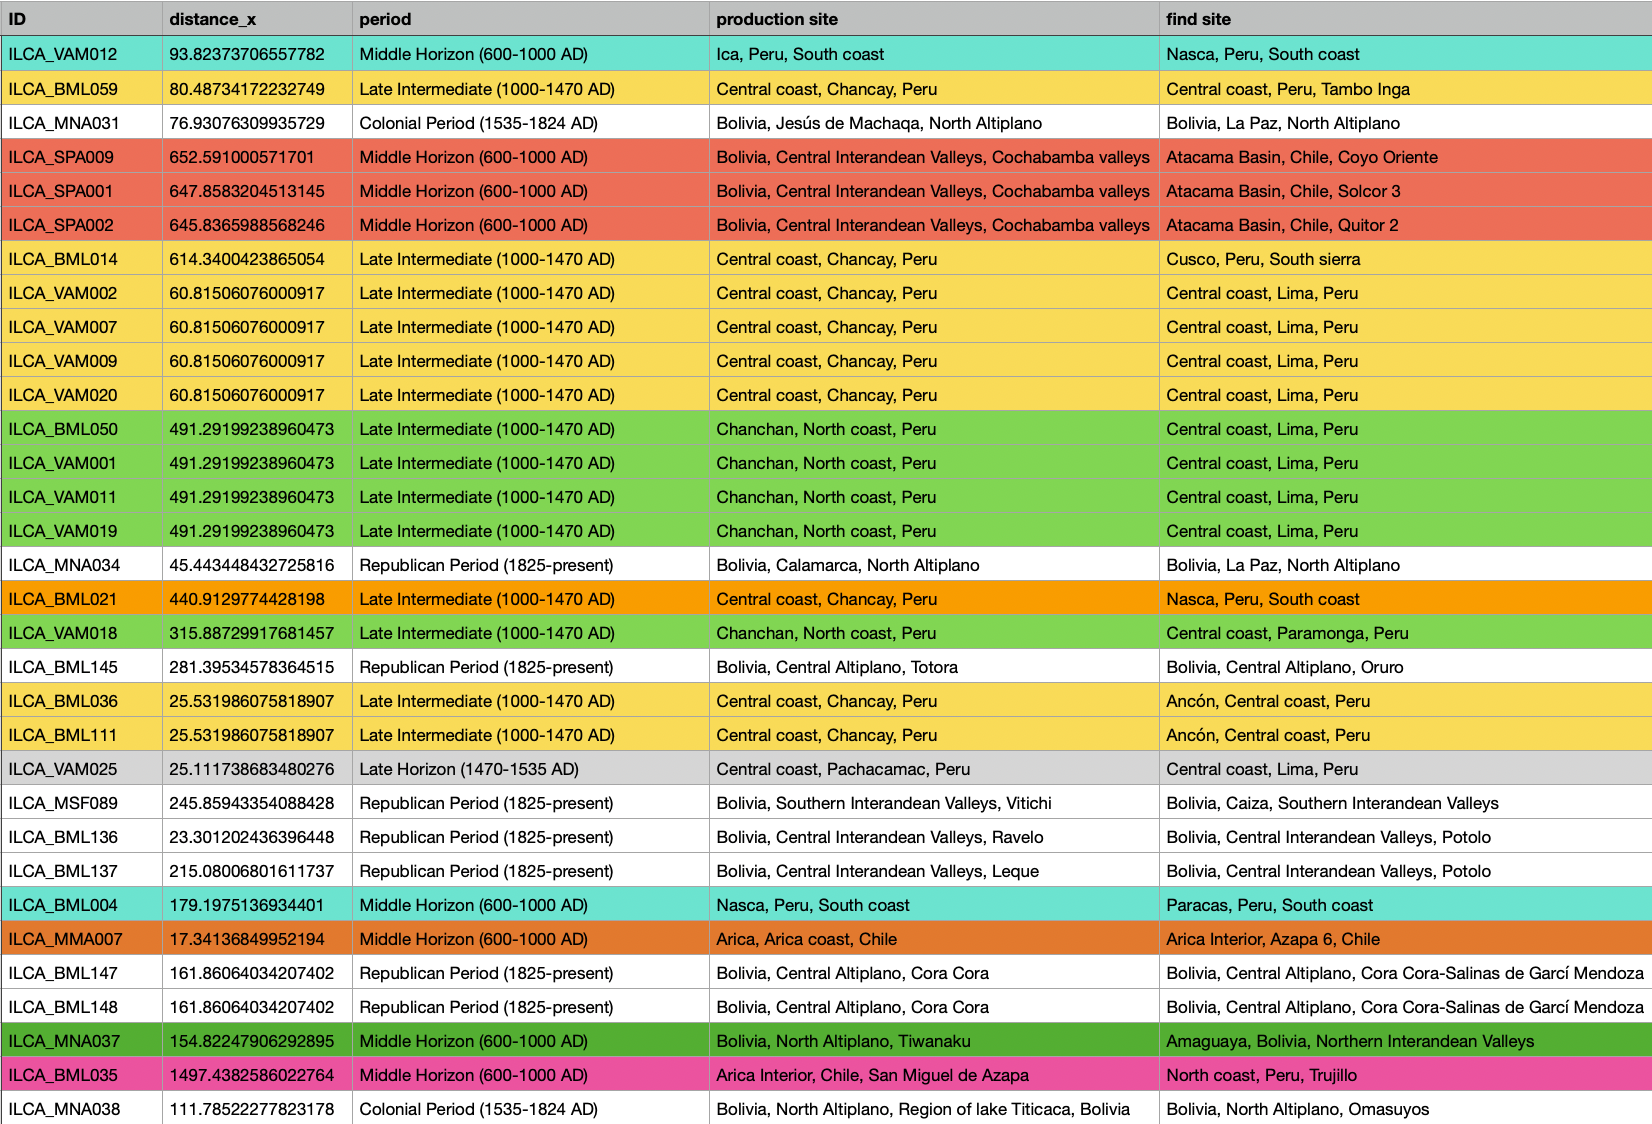
\includegraphics[width=16cm]{../images/tabDistance.png}
		\caption{Tableau des cas de textiles dont le lieu de découverte est à plus de 5 kilomètres \\ de son lieu de production. Les couleurs indiquent des mobilités géographiquement similaires.}
		\label{fig:distancetab}
	 \end{center}
\end{figure}

\clearpage

\begin{wrapfigure}{l}{0.2\textwidth}
    \centering
    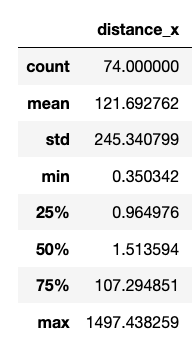
\includegraphics[width=0.2\textwidth]{../images/stat_distance.png}
    \label{fig:distance}
\end{wrapfigure}

\noindent Sur les 696 textiles référencés dans la base de données, 74 ont un lieu de découverte distinct de leur lieu de production. La distance moyenne séparant le lieu de découverte et le lieu de production dans le cas où ils sont distincts est de 121,70 kilomètres, la plus petite étant de 350 mètres et la plus grande de 1497,44 kilomètres. Toutefois, la médiane est à 1,51 kilomètre. Les distances sont donc plutôt réduites et les plus petites distances sont probablement liées à la géolocalisation. Par exemple, les textiles découverts à \textit{Playa Miller} ont été produits à Arica soit à 1 kilomètre de leur lieu d'excavation. Il en est de même pour les textiles provenant des fosses d'Azapa qui ont été produites à San Miguel de Azapa, à 1,5 kilomètres de là. Ces cas dont le lieu de découverte est situé à moins de 5 kilomètres du lieu de production sont au nombre de 42, nous avons décidé de les supprimer de la représentation graphique pour ne pas surcharger la carte et pour se concentrer sur les textiles qui ont plus amplement circulé. Nous obtenons alors une liste de 32 textiles dont les lieux de découverte sont à plus de 5 kilomètres de leurs lieux de production.

\noindent Dans notre base de données, ces mobilités apparaissent à partir de l'Horizon Moyen (600 avant J.C.) et s'étendent jusqu'à la période républicaine. Les mobilités semblent plus intenses au cours de l'Horizon Moyen et de la période Intermédiaire Récente. 
L'Horizon Récent ne présente qu'un seul cas de mobilité physique avec un textile produit à Pachacamac et découvert à Lima (en gris dans le tableau \ref{fig:distancetab}). Pachacamac était un centre administratif et religieux central de la période Intermédiaire Ancienne à l'empire Inca, et son influence portait sur la région de Lima. Il n'est donc pas surprenant que ce textile se trouve ainsi à 25 kilomètres de son lieu de production. 

Au cours de l'Horizon Moyen, plusieurs textiles voyagent depuis les hautes-terres boliviennes vers le bassin de l'Atacama au nord du Chili (en rouge dans le tableau \ref{fig:distancetab}), soit plus de 600 kilomètres de distance. Ces trois textiles sont de style Tiwanaku et confortent l'hypothèse d'une influence de l'empire Tiwanaku sur le sud de la zone andine que nous avons déjà souligné avec l'exemple \ref{fig:MNA037}. Le travail d'Alex Nielsen sur la circulation d'objets atteste des routes commerciales entre ces deux zones\footnote{\cite[p.~407]{nielsenCirculatingObjectsConstitution2013}, voir figure 16.16}. En outre, les tuniques locales d'Atacama imitent des textiles Tiwanaku, probablement à partir des modèles qui sont arrivés depuis les hautes-terres boliviennes. La comparaison de ces exemples est d'autant plus intéressante qu'elle semble illustrer le phénomène d'imitation dont nous parlions dans le premier chapitre du mémoire. En effet, les manches du textile SPA012 (photographie \ref{fig:SPA012}) de style Tiwanaku sont réalisées en broderie. Or, dans le cas du textile qui vient des hautes-terres ce même type de motif est réalisé en tresses adjointes au tissage à dominante chaîne. % A vérifier 
Il pourrait donc s'agir d'une imitation iconographique en modifiant la technique\footnote{Cette hypothèse mériterait d'être vérifiée, d'une part en ayant accès au textile pour les caractéristiques techniques, et d'autre part en le comparant à d'autres cas similaires.}.

\begin{figure}[!h]
    \begin{minipage}[c]{.5\linewidth}
            \begin{center}
                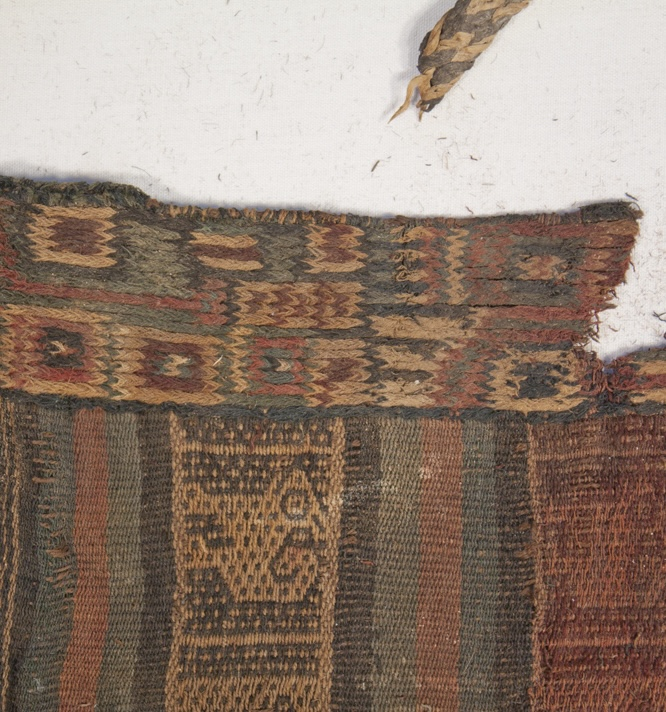
\includegraphics[height=7cm]{../images/SPA009.jpg}
            \end{center}
            \caption{Détail d'un textile Tiwanaku produit dans les hautes-terres et découverts dans le bassin de l'Atacama (Horizon Moyen). Référence dans la base de données : SPA009.}
            \label{fig:SPA009}   
    \end{minipage}
\hspace{5pt}
        \begin{minipage}[c]{.5\linewidth}
        \begin{center}
        		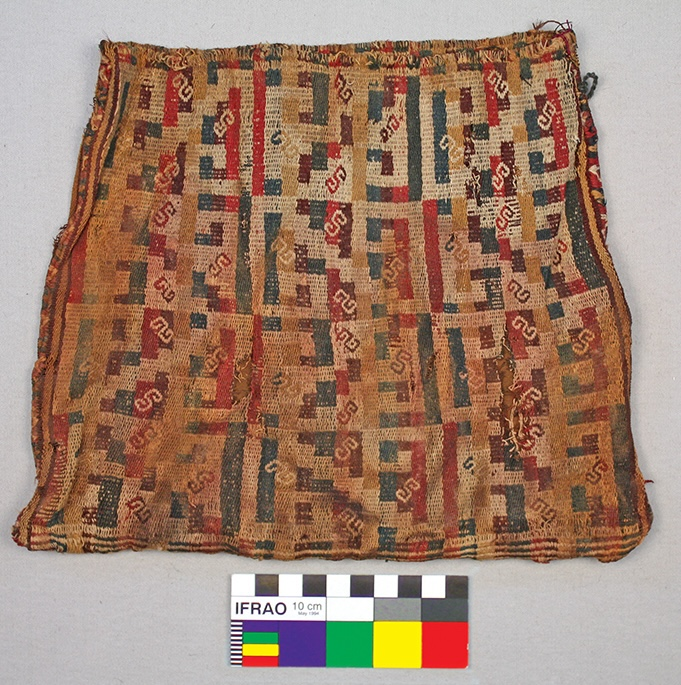
\includegraphics[height=7cm]{../images/BML035.jpg}
	\end{center}
	\caption{Sac produit à Azapa et découvert à Trujillo (Horizon Moyen). \\ Référence dans la base de données : BML035}
	\label{fig:BML035}
    \end{minipage}
\end{figure}

\noindent À la même période, sur la côte sud du Pérou des textiles circulent entre Ica, Nazca et Paracas (en bleu dans le tableau \ref{fig:distancetab}). Ces trois zones sont très proches et il n'est pas surprenant que les textiles des civilisations locales s'échangent dans cette zone. D'autant plus que les deux textiles référencés sont de style Nazca-Huari (photographie \ref{fig:VAM012}), s'inscrivant donc dans l'aire d'influence commune de l'empire Huari.
Enfin, un textile sort du lot (en rose dans le tableau \ref{fig:distancetab}), il s'agit d'un sac cérémoniel destiné à la coca, dans un style local d'Azapa (côte nord du Chili) découvert à Trujillo (nord du Chili), soit à 1497,44 kilomètres de son lieu de production. Ce textile est très mystérieux et je ne suis pas en mesure d'expliquer le trajet qu'il a pu effectuer entre son point de départ et son point d'arrivée. Son rôle religieux pourrait expliquer sa circulation. Il confirme la réalité des échanges textiles sur la longue distance dans la zone andine.

\begin{wrapfigure}{r}{0.6\textwidth}
    \centering
    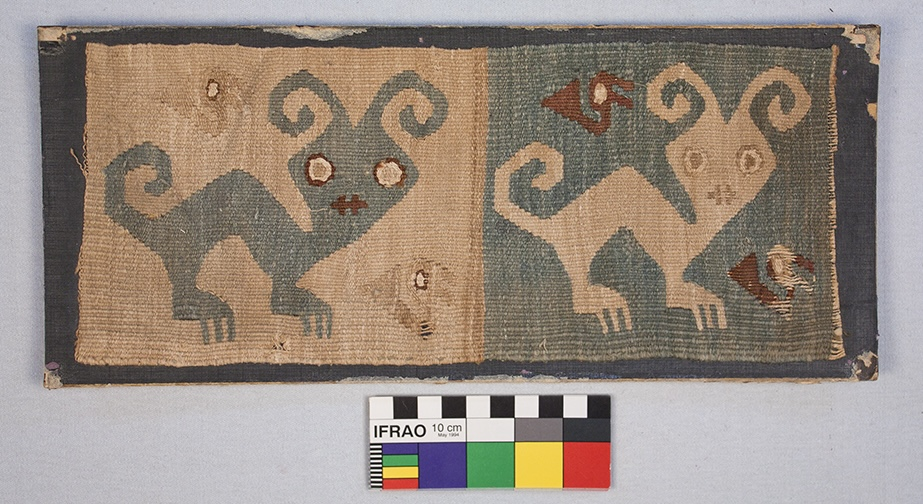
\includegraphics[width=0.6\textwidth]{../images/BML014.jpg}
    \caption{Fragment Chancay retrouvé à Cuzco. \\ Référence dans la base de données : BML014}
    \label{fig:BML014}
\end{wrapfigure}

À la période Intermédiaire Récente, deux types de mobilités apparaissent. Les textiles qui circulent au sein de la côte centrale (en jaune dans le tableau \ref{fig:distancetab}) et les textiles qui circulent entre la côte centrale et la côte nord (en vert dans le tableau \ref{fig:distancetab}). Dans le premier cas, il s'agit de textiles dont la mobilité fait moins de 100 kilomètres. Ce sont des tissus Chancay retrouvés à Lima, soit dans la zone d'influence de cette civilisation\footcite[p.~72]{boissiereAtlasAmeriquePrecolombienne2022}.
 Il en est de même pour les textiles Chimú de la côte nord du Pérou, qui sont originaires de la capitale Chan Chan et découverts à Lima, soit près de 500 kilomètres plus au sud mais dans l'aire d'influence de cette civilisation.
Un cas se distingue à cette période, le fragment BML014, textile Chancay retrouvé à Cuzco. De la même manière, son parcours et ses conditions de conservation ne sont pas spécifiées mais il pourrait être l'indice d'une circulation des textiles sur de longues distances à cette période.

Les derniers cas (en blanc dans le tableau \ref{fig:distancetab}) sont les textiles post-coloniaux. Ils composent la quasi-totalité des mobilités inter-andines des hautes-terres boliviennes (voir carte \ref{fig:distance_map}). Là non plus, nous n'avons pas leur parcours et nous ne pouvons donc que proposer des hypothèses quant à leur circulation. À partir de la période coloniale, les relations marchandes se développent de manière croissante dans les Andes, notamment les échanges commerciaux de textiles. Ces échanges marchands sont la première hypothèse de circulation des textiles dans cette zone, notamment pour les textiles retrouvés à La Paz, capitale bolivienne au c\oe{}ur des échanges économiques du pays.

Nous pouvons observer sur la carte suivante, pour les 32 cas étudiés, les lieux de production, les lieux de découverte et la distance à vol d'oiseau qui les sépare (en vert). Grâce au paramètre \textit{alpha} des couleurs dans la librairie Python Matplotlib nous avons pu ajouter de la transparence pour garder une information de densité. Ainsi, les points les plus intenses indiquent une multitude de textiles et les points violets indiquent qu'un lieu est à la fois origine et destination des textiles.

\begin{figure}[!h]
	\begin{center}
		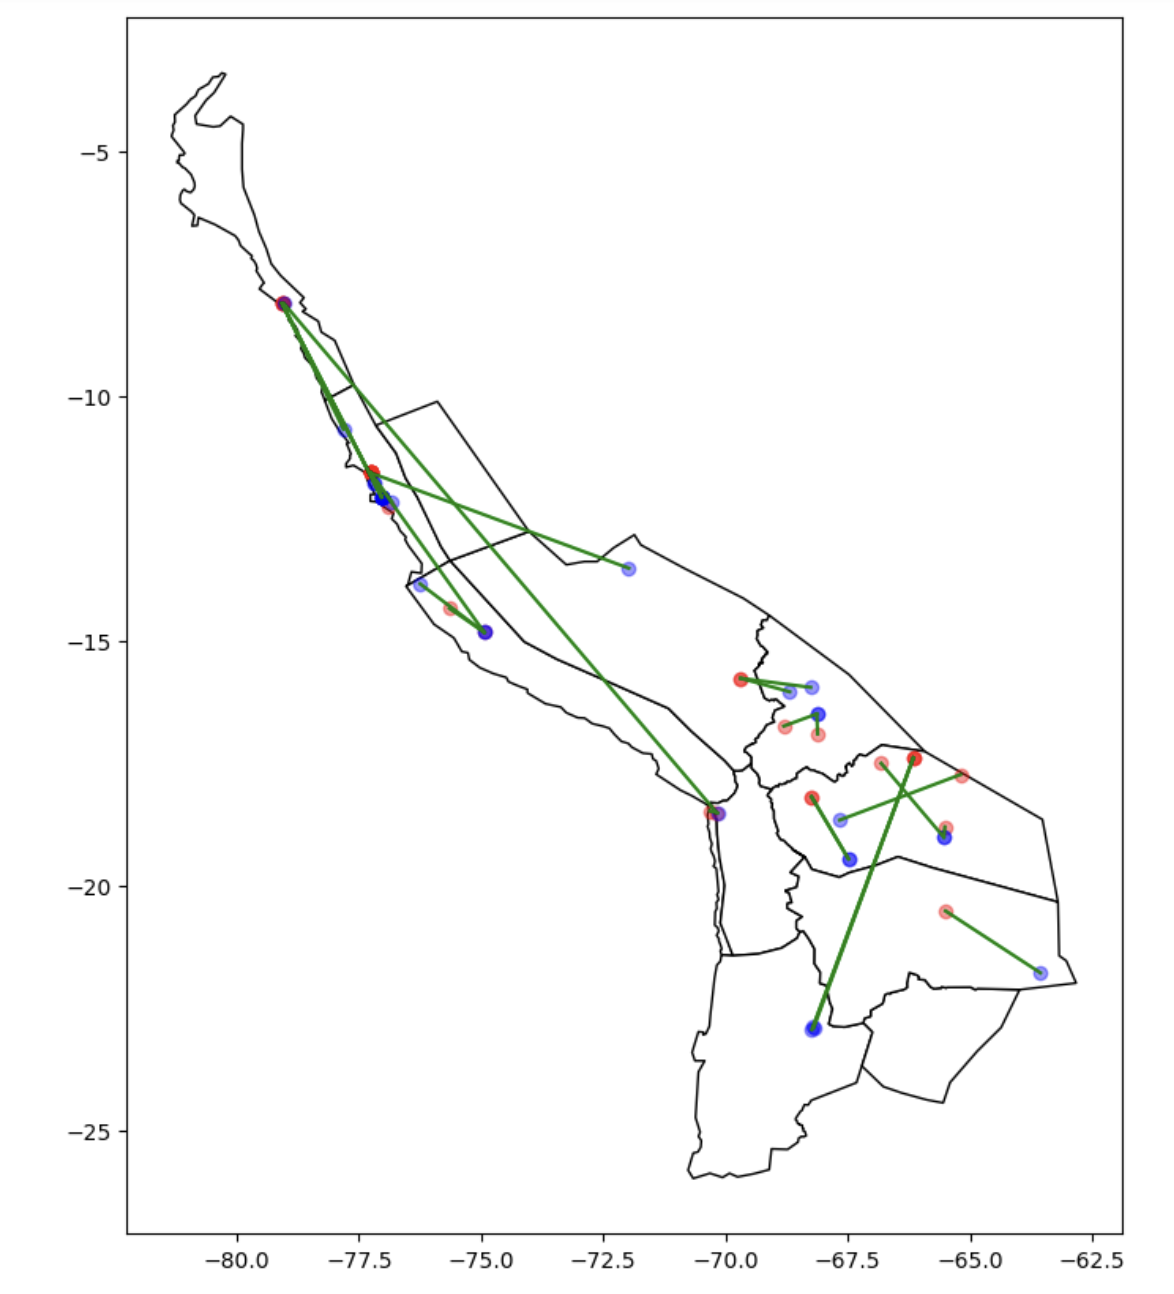
\includegraphics[width=15cm]{../images/carteDistance.png}
		\caption{Carte reprenant les distances entre les lieux de production (en rouge) et les lieux de découverte (en bleu) des textiles.}
		\label{fig:distance_map}
	 \end{center}
\end{figure}

Après un large travail d'homogénéisation des données en ligne avec l'état de l'art, nous avons pu proposer une première analyse géographique diachronique des textiles du corpus. Ces cartographies confirment la répartition des textiles sur le territoire andin tel qu'expliqué par les conditions de conservation et par le développement des civilisations sur le territoire. En outre, le géocodage des lieux de production et de découverte des textiles nous ont permis de mettre au jour des mobilités plus ou moins intenses entre civilisations pré-hispaniques. Néanmoins, l'analyse des métadonnées des textiles ne nous permet pas de saisir les évolutions iconographiques des textiles. C'est pourquoi dans le dernier temps du mémoire, nous allons nous appuyer sur le corpus de photographies de la base de données \textit{Weaving Communities of Practice} afin de tester nos hypothèses d'imitations techniques et iconographiques.